\documentclass[master]{NTHUthesis}
\usepackage[utf8]{inputenc}

%%% Customization  %%%
\usepackage{graphicx}           % figures
\usepackage{amsmath}            % for \text in math mode
\usepackage{amssymb}            % for \mathbb and additional math symbols
\usepackage{microtype}          % improve justification; reduce overfull/underfull boxes
\usepackage{booktabs}           % tables
\usepackage[ruled]{algorithm2e} % algorithms, list of algorithms
\usepackage{cite}               % bibliography
\usepackage{braket}             % for \braket command
\usepackage{array}              % tabularx column helpers
\usepackage{tabularx}           % better full-width tables
\usepackage{longtable}          % multi-page tables (appendix literature schema)
\usepackage{placeins}           % \FloatBarrier to control float drift
\usepackage{listings}           % code listings (appendix configs)

\definecolor{teal}{rgb}{0.0,0.5,0.5}

\lstdefinelanguage{yaml}{
  keywords={true,false,null,y,n},
  keywordstyle=\color{blue}\bfseries,
  sensitive=false,
  comment=[l]{\#},
  commentstyle=\color{gray}\ttfamily,
  stringstyle=\color{teal},
  morestring=[b]',
  morestring=[b]"
}

\lstdefinestyle{yamlStyle}{
  language=yaml,
  basicstyle=\ttfamily\footnotesize,
  columns=fullflexible,
  breaklines=true,
  showstringspaces=false,
  frame=single,
  rulecolor=\color{black!20},
  backgroundcolor=\color{black!2}
}

\setlength{\emergencystretch}{2em}


%%% Necessary %%%
\titleZH{基於物理資訊之稀疏量測湍流重建在公開基準資料集上的評估與分析}
\titleEN{Evaluation and Analysis of Physics-Informed Turbulence Reconstruction from Sparse Measurements on Public Turbulence Benchmarks}
\instituteZH{工程與系統科學研究所乙組}
\studentID{113011527}
\studentZH{李駿毅}
\studentEN{JunYi Li}
\advisorZH{林洸銓}
\advisorEN{Kuang C. Lin}
\yearZH{115}
\monthZH{6}

\begin{document}
\begin{CJK*}{UTF8}{bsmi}

\makecover

\pagenumbering{Roman}

%%% Abstract (Chinese) %%%
\begin{abstractZH}
本研究提出一個基於物理先驗的 PINNs（Physics-Informed Neural Networks）逆問題框架，針對湍流流場的重建與誤差分析進行探討。
與既有方法需依賴大量完整資料不同，本研究以極為稀疏的觀測點（$K = 100$，僅占全場網格極小比例），結合物理方程與列主元 QR 分解（QRCP）選點策略，模擬工程情境中「先有低保真 RANS/粗網格模擬，再決定感測器佈置，再取得少量高保真實測」的工作流程，並將公共湍流資料庫視為高保真參考場。
在方法層面，本研究設計了一套可結合低保真 RANS 模擬作為軟先驗（soft prior）的 VS-PINN 架構；在數值實驗中，則以 QR 選點搭配前向 VS-PINN 訓練，在 2D Kolmogorov flow 與 JHTDB 通道流（$Re_\tau \approx 1000$）上建立可重現的基準結果。本論文以 DNS/JHTDB 作為可控且可重現的高保真參考場，並以其在感測點上的取樣（可視需求加入合成噪聲）替代實驗量測，用於系統性評估感測器佈置與重建性能；實務部署時，DNS 將由實際感測數據取代。
結果顯示，在目前的設定下，PINNs 能在感測點極度稀疏的情況下重建部分關鍵流場結構，並提供與 DNS 對照的一致評估流程。具體而言，本論文在 2D Kolmogorov flow 上提供了低保真先驗對重建品質的消融對比；在 3D JHTDB 通道流部分，低保真 RANS 用於感測器佈置與提供候選先驗，而本文先以 prior 權重設為 0 的 baseline 呈現極端稀疏下的重建難點，並保留後續啟用 prior 之擴充空間。
\end{abstractZH}

%%% Optional %%%
%\begin{acknowledgementsZH}
%\zhlipsum[1-2]
%\end{acknowledgementsZH}

%%% Abstract (English) %%%
\begin{abstractEN}
This study proposes a Physics-Informed Neural Networks (PINNs) framework for turbulence inversion from sparse measurements in an engineering-oriented setting, where only inexpensive low-fidelity simulations are available at sensor-design time and high-fidelity data are scarce.
Unlike conventional approaches that rely on abundant datasets, the proposed framework leverages very sparse observations ($K = 100$) together with the governing Navier--Stokes equations and QR-based sensor placement applied to low-fidelity baseline fields (e.g., RANS or coarse DNS/LES), and uses public benchmark datasets such as 2D Kolmogorov flow and the JHTDB channel-flow DNS at $Re_\tau \approx 1000$ as controllable surrogates for experimental measurements and full-field reference.
On the modeling side, we design a VS-PINN architecture that incorporates low-fidelity simulations (e.g., RANS) as soft priors and uses low-fidelity fields for QR-based sensor placement. In the reported experiments, we (i) provide a prior ablation on 2D Kolmogorov flow (vanilla vs.\ soft prior variants under matched sensor layouts) and (ii) report a 3D JHTDB channel-flow baseline under the same multi-fidelity pipeline, where RANS guides sensor placement and the prior term is treated as an ablation knob (the reported baseline sets its weight to zero) while keeping DNS strictly in the role of a reference field for virtual sensing and evaluation.
Throughout, virtual sensor observations are sampled from DNS (noise-free by default, optionally with synthetic noise) to systematically evaluate sensor placement and reconstruction performance; in practical deployment, the same pipeline applies with DNS replaced by real sensor data.
The results show that, under extreme sparsity, the baseline PINN reconstructions recover some qualitative large-scale structures and enable consistent a posteriori evaluation against DNS, while quantitative accuracy remains challenging at the current sensor budget; systematic improvements will be pursued in subsequent work.
\end{abstractEN}

%%% Optional%%%
%\begin{acknowledgementsEN}
%\lipsum[1-2]
%\end{acknowledgementsEN}

%%% Necessary %%%
\begingroup
\sloppy
\hbadness=10000
\vbadness=10000
\hfuzz=10pt
\vfuzz=10pt
\maketoc
\endgroup

%%% Notation \& Abbreviations %%%
\chapter*{Abbreviations and Notation}
\addcontentsline{toc}{chapter}{Abbreviations and Notation}

\noindent\textbf{Abbreviations}

\begin{tabular}{ll}
PINNs & Physics-Informed Neural Networks \\
HFM   & Hidden Fluid Mechanics \\
DNS   & Direct Numerical Simulation \\
LES   & Large-Eddy Simulation \\
RANS  & Reynolds-Averaged Navier--Stokes \\
JHTDB & Johns Hopkins Turbulence Database \\
PIV   & Particle Image Velocimetry \\
VS-PINN & Variable-Scaling PINN \\
QRCP  & QR with Column Pivoting \\
QR-DEIM & QR Discrete Empirical Interpolation Method \\
PDE   & Partial Differential Equation \\
NS    & Navier--Stokes \\
CFD   & Computational Fluid Dynamics \\
SOAP  & Second-Order Algorithm for Preconditioning \\
\end{tabular}

\vspace{1em}
\noindent\textbf{Notation}

\begin{tabular}{ll}
$\mathbf{x} = (x,y,z)^T$ & Spatial coordinates in the channel domain \\
$t$ & Time \\
$\Omega$ & Spatial domain, $[0,L_x]\times[-h,h]\times[0,L_z]$ \\
$\mathbf{u} = (u,v,w)^T$ & Instantaneous velocity field \\
$p$ & Instantaneous pressure field \\
$\mathbf{S} = (S_x,S_y,S_z)^T$ & Learnable source term in the momentum equations \\
$\rho$ & Fluid density \\
$\nu$ & Kinematic viscosity \\
$Re$ & Reynolds number \\
$Re_\tau$ & Friction Reynolds number \\
$k_f$ & Forcing wavenumber in Kolmogorov flow \\
$\mathbf{u}_{\text{RANS}}$ & RANS mean velocity field used as low-fidelity prior \\
$\phi^{\text{HF}}$ & High-fidelity (PINN) prediction of a flow variable \\
$\phi^{\text{LF}}$ & Low-fidelity prior value of a flow variable \\
$\mathcal{L}_{\text{data}}$ & Data consistency loss on sparse sensors \\
$\mathcal{L}_{\text{pde}}$ & Physics residual loss (Navier--Stokes and continuity) \\
$\mathcal{L}_{\text{bc}}$ & Boundary-condition loss (no-slip, periodicity) \\
$\mathcal{L}_{\text{prior}}$ & Prior consistency loss with low-fidelity data \\
$\mathcal{L}_{\text{reg}}$ & Regularization loss on the source term $\mathbf{S}$ \\
$N_{\text{sensor}}$ & Number of sparse sensor measurements \\
$N_{\text{pde}}$ & Number of collocation points for PDE residuals \\
$N_{\text{prior}}$ & Number of collocation points for prior consistency loss \\
$\mathbf{N}=(N_x,N_y,N_z)$ & Anisotropic scaling factors in VS-PINN \\
\end{tabular}

%%% Optional %%%
%\phantomsection
%\listofalgorithms
%\addcontentsline{toc}{chapter}{List of Algorithms}
%\clearpage

\pagenumbering{arabic}

\chapter{Introduction}

\section{Background}
Turbulence is multiscale, nonlinear, and chaotic, making high-Reynolds-number prediction costly. Direct numerical simulation (DNS) at high $Re$ is often infeasible, while experiments (e.g., planar/volumetric PIV) provide only sparse, noisy, partial-field observations. Conversely, low-fidelity closures (RANS, coarse LES) are affordable but systematically biased in mean profiles, second-order statistics, and spectra. Practical workflows therefore face a persistent mismatch between the data needed for full-field inference and the data typically available.

\paragraph{Stance on DNS and measurements.}
Throughout this thesis, DNS (e.g., JHTDB) is treated as a controllable and reproducible surrogate for measurements: sparse observations are generated by sampling the DNS field at designed sensor locations (optionally with additive synthetic noise), while the full DNS field is used only as a reference for a posteriori evaluation. In practical deployment, the same workflow applies with DNS replaced by real sensor data.

Before the advent of PINNs, missing or incomplete turbulent fields were typically reconstructed using statistical interpolation or data-assimilation techniques such as Kriging, Gappy POD, and variational/Kalman-filter-based assimilation. These methods exploit correlations or linearized dynamics but either ignore the full nonlinear Navier--Stokes physics or become prohibitively expensive when enforcing PDE constraints in 3D high-$Re$ flows, especially under extremely sparse sensing.

Physics-Informed Neural Networks (PINNs) embed governing laws (e.g., incompressible Navier--Stokes) into a differentiable loss, enabling physics-regularized inference from limited observations~\cite{Raissi2019JCP, Karniadakis2021NRP}. Since Raissi \emph{et al.} (2019)~\cite{Raissi2019JCP}, much of the literature has focused on \emph{forward} benchmarks, where PINNs compete with mature CFD solvers. However, PINNs are often most practically distinctive in \emph{inverse} and data-assimilation problems, where unknown quantities include not only the flow state but also parameters, forcing, boundary conditions, or hidden fields constrained only indirectly by measurements. Hidden Fluid Mechanics (HFM) is a canonical example: by augmenting the momentum equations with a learnable source term, HFM uses PINNs to infer velocity, pressure, and forcing from shadowgraphy-like visualizations, without requiring a conventional forward solve in the usual sense~\cite{Raissi2020Science}. In such inverse settings, traditional numerical solvers are not directly applicable without substantial wrapper algorithms (e.g., adjoint-based optimization, ensemble Kalman filters, or variational DA), and the cost of repeatedly solving high-dimensional PDEs can become prohibitive.

For turbulence, engineering questions are often inverse: reconstructing fields from a few probes, correcting biased RANS/coarse LES with sparse data, or identifying effective source terms. Recent work has also shown that PINNs can simulate fully turbulent flows in 3D~\cite{wang2025simulatingthreedimensionalturbulencephysicsinformed}, yielding stabilization insights relevant to inverse problems. This thesis focuses on two practical constraints in turbulent inverse settings: (i) sensor placement under extreme sparsity and (ii) training stability for stiff, broadband 3D losses.

\paragraph{Implementation validation (prior work).}
To de-risk the main turbulence benchmarks, we first validated our Navier--Stokes PINN pipeline on a canonical high-$Re$ lid-driven cavity benchmark, motivated by the solution multiplicity and data-effect analysis of Wang et al.\ (2023)~\cite{wang2023solutionmultiplicityeffectsdata}. We reproduced a physics-only baseline and further added a sparse-supervision extension (10 labeled points) to quantify how minimal data affect convergence cost in an already-regularized formulation. A concise summary (one table + one figure) is provided in Appendix~\ref{appendix:wang2023_repro}.

\section{Literature Review}
\label{sec:literature_review}

This literature review is \emph{comparison-driven}. It is not intended as an exhaustive survey or a leaderboard of state-of-the-art accuracy; rather, it organizes prior work around design choices that determine identifiability and reproducibility under sparse observations. We focus on sparse reconstruction of high-$Re$ wall-bounded turbulence (3D channel flow) with PINNs, in workflows where low-fidelity simulations (e.g., RANS) are available for sensor design and soft regularization. We compare prior work by flow/target, observation modality and sparsity definition, physics constraints (NS vs.\ RANS/closure-aware), and the role of low-fidelity information. Throughout, citations use last names only (two authors: both names; three or more: ``et al.''), with venue abbreviations (PoF, Exp.\ Fluids, PNAS, arXiv) where helpful.

\subsection{Overview of Sparse Turbulence Reconstruction Methods}
\label{sec:literature_overview}

We group the most relevant studies into three complementary lines aligned with this thesis: (1) channel-/wall-bounded state estimation from sparse observations, (2) RANS/turbulence-model-augmented PINNs for mean-flow or closure-aware inference, and (3) generic sparse-sensor reconstruction beyond channel flow. Two cross-cutting axes recur across all three lines and are therefore treated explicitly in this chapter: (i) how observation budgets are reported and normalized, and (ii) whether sensor placement is assumed or designed (and from what information). Table~\ref{tab:reconstruction_methods} summarizes representative works in a unified comparison format.

\begin{table}[!htbp]
	    \centering
	    \caption{Representative sparse-reconstruction studies compared along the chapter axes.}
	    \label{tab:reconstruction_methods}
	    \footnotesize
        \setlength{\tabcolsep}{3pt}
        \renewcommand{\arraystretch}{1.15}
	    \begin{tabularx}{\textwidth}{
	        >{\raggedright\arraybackslash}p{2.4cm}
            >{\raggedright\arraybackslash}p{2.2cm}
            >{\raggedright\arraybackslash}p{2.3cm}
            >{\raggedright\arraybackslash}p{2.1cm}
            >{\raggedright\arraybackslash}p{1.8cm}
            X
	    }
	    \toprule
		    \textbf{Reference (venue)} & \textbf{Flow \& target} & \textbf{Observations (sparsity)} & \textbf{Constraints \& prior} & \textbf{Sensor placement} & \textbf{Outcome (metrics, limitation)} \\
	    \midrule
		    Du et al.\ (arXiv)~\cite{du2022stateestimationminimalturbulent} & Minimal turbulent channel; instantaneous (infer $p$) & Spatio-temporal sparse Eulerian $u$ (mask over window) & NS; no low-fidelity prior & Given (mask) & PINN vs.\ 4DVar; adjoint-free but sensitive to training; limited beyond assimilation window \\
		    Clark Di Leoni et al.\ (Exp.\ Fluids)~\cite{Clark_Di_Leoni_2023} & Turbulent fields; instantaneous $u,p$ & Noisy under-resolved Lagrangian tracks & NS; no low-fidelity prior & Given tracks & Robust to sparse/noisy tracks; budgets reported via track density/noise (not a single $K/N$) \\
		    Shin \& Schr{\"o}der\ (ISPIV)~\cite{shin2025robust} & HIT/channel (DNS) + TBL (exp.); velocity & LPT density sweep & NS-regularized; robustness emphasis & Given tracks & Sensitivity to modality, particle density, and noise; motivates budget reporting beyond $K$ \\
		    Patel et al.\ (arXiv)~\cite{patel2024turbulencemodelaugmentedphysics} & Periodic hill; mean flow & Sparse mean velocity (pointwise) & RANS (+SA); closure-aware prior & Given sites & Turbulence-model augmentation reduces data needs for mean-flow reconstruction; less direct for instantaneous channel \\
		    von Saldern et al.\ (PoF)~\cite{von_Saldern_2022} & Mean-flow DA; hidden quantities & Sparse mean fields (LES/PIV) & Mean constraints; identify hidden/closure terms & Given coverage & Consistent mean states under sparse data; sparsity often not reducible to a unified $K/N$ \\
		    Pioch et al.\ (Fluids)~\cite{fluids8020043} & Backward-facing step; mean / closure sensitivity & Sparse labeled profiles/lines & RANS-based PINN; closure choice matters & Given labels & Strong dependence on closure choice; illustrates bias risk under strong priors \\
		    Hosseini \& Shiri\ (PoF)~\cite{10.1063/5.0211680} & Sparse-sensor reconstruction benchmarks & Sparse Eulerian sensors & PDE-constrained inverse PINN & As given & Direct sparse-sensor baseline; useful for calibrating sparsity regimes and reporting conventions \\
		    Chaurasia \& Chakraborty\ (PoF)~\cite{10.1063/5.0218611} & Turbulent reconstruction examples & Sparse Eulerian measurements & PDE-constrained inverse PINN & As given & Highlights sparse turbulent regimes and robustness; sensor-design rationale limited for $K\!\ll\!N$ \\
	    \bottomrule
	    \end{tabularx}
\end{table}
\FloatBarrier

Across these works, sparse reconstruction is ill-posed without strong regularization. PINNs regularize through PDE constraints, but performance depends on how sparsity is defined, how observations are distributed, and how low-fidelity information is incorporated. The remainder of this section narrows to channel-flow--centric comparisons and identifies what is still missing for a reproducible high-$Re_\tau$ workflow under extreme sparsity.

\subsection{Sensor Budget and Reconstruction Accuracy Targets}
\label{sec:sensor_budget_targets}

Sparse-flow papers report ``data budgets'' inconsistently (points per frame, percent of a grid, or mixed IC/BC/data counts), which complicates cross-paper comparisons. For a comparable engineering view, we describe observation budgets by: (i) spatial sparsity $K/N$, (ii) temporal coverage $N_t$, and (iii) observation dimensionality $d_{\text{obs}}$. For Eulerian sensing, the observed scalar budget is
\begin{equation}
    \label{eq:obs_dof_def}
    N_{\text{obs}} = K\,N_t\,d_{\text{obs}}.
\end{equation}
For Lagrangian tracking, an analogous $N_{\text{obs}}$ follows from particles/frame $\times$ frames $\times d_{\text{obs}}$, together with the noise level. Importantly, not all modalities admit a clean mapping to a single, grid-normalized $K/N$; when required budget descriptors are not reported, we mark them as \textbf{NR} and treat this as a reporting gap rather than imputing values.

\begin{table}[!htbp]
    \centering
    \caption{How representative studies report observation budgets ($K/N$, $N_t$, $d_{\text{obs}}$, $N_{\text{obs}}$).}
    \label{tab:obs_budget_literature}
    \footnotesize
    \begin{tabularx}{\textwidth}{
        >{\raggedright\arraybackslash}p{3.6cm}
        >{\raggedright\arraybackslash}p{3.0cm}
        >{\raggedright\arraybackslash}p{3.0cm}
        X
    }
    \toprule
    \textbf{Reference} & \textbf{Flow / target} & \textbf{Observations} & \textbf{Budget descriptors (as reported / normalized)} \\
    \midrule
    Du et al.\ (arXiv)~\cite{du2022stateestimationminimalturbulent} & Minimal turbulent channel; state estimation & Spatio-temporal sparse Eulerian velocity & Defines sparsity through an observation mask over an assimilation window; $K/N$ and $N_t$ depend on the mask design and time horizon \\
    Clark Di Leoni et al.\ (Exp.\ Fluids)~\cite{Clark_Di_Leoni_2023} & Turbulent fields; reconstruct Eulerian $u,p$ & Noisy Lagrangian particle tracks & Reported via particle-track density and measurement noise; an effective $N_{\text{obs}}$ scales with particles/frame $\times$ frames $\times d_{\text{obs}}$ \\
    Shin \& Schr{\"o}der\ (ISPIV)~\cite{shin2025robust} & LPT reconstruction; robustness study & Lagrangian particle tracking (LPT) & $\sim$54{,}000 particles/frame (varied); emphasizes reconstruction sensitivity to particle density, modality, and noise \\
    Patel et al.\ (arXiv)~\cite{patel2024turbulencemodelaugmentedphysics} & Turbulent periodic hill; mean-flow reconstruction & Sparse pointwise mean velocity & Varies measurement resolution; compares PINN vs variational DA under identical sparse mean-field constraints (mean-flow setting: $N_t$ not central) \\
    von Saldern et al.\ (PoF)~\cite{von_Saldern_2022} & Mean-flow assimilation; hidden quantities/closure & Sparse mean fields (LES/PIV) & Sparse mean-field coverage; focuses on identifying inaccessible variables/closure-related quantities rather than reporting a single $K/N$ \\
    Hosseini \& Shiri\ (PoF)~\cite{10.1063/5.0211680} & Flow-field reconstruction & Sparse sensors (Eulerian) & Directly targets sparse-sensor reconstruction; useful for calibrating sparsity regimes and reporting conventions \\
    Chaurasia \& Chakraborty\ (PoF)~\cite{10.1063/5.0218611} & Turbulent reconstruction under sparse data & Sparse measurements (Eulerian) & Turbulent reconstruction examples under sparse measurements; useful for discussing robustness and failure modes at low $N_{\text{obs}}$ \\
    \bottomrule
    \end{tabularx}
\end{table}
\FloatBarrier

\begin{table}[!htbp]
    \centering
    \caption{Common evaluation metrics for sparse turbulence reconstruction (beyond global field norms).}
    \label{tab:recon_metrics}
    \footnotesize
    \begin{tabularx}{\textwidth}{
        >{\raggedright\arraybackslash}p{3.1cm}
        >{\raggedright\arraybackslash}p{4.2cm}
        >{\raggedright\arraybackslash}p{2.6cm}
        X
    }
    \toprule
    \textbf{Metric family} & \textbf{Definition (informal)} & \textbf{Target} & \textbf{Purpose / notes (representative refs.)} \\
    \midrule
    Field-level norms ($L_2$/NRMSE/MAPE) & Global error on $u,v,w,p$ (continuous or discrete) & Instantaneous / mean & Baseline comparability metric but can hide spectral/near-wall failures~\cite{shin2025robust, 10.1063/5.0180770} \\
    Divergence error ($\|\nabla\!\cdot\!u\|$) & Mean/max incompressibility residual & Instantaneous & Diagnoses whether physics satisfaction is meaningful under sparse data (important when solutions over-smooth) \\
    Mean-profile error ($U^+(y^+)$, $\langle u\rangle$) & Deviation of mean velocity profile from reference & Mean / statistics & Engineering-relevant for wall flows; detects collapse to mean-profile/trivial solutions \\
    Wall shear / friction velocity ($\tau_w$, $u_\tau$) & Error in wall stress or derived friction velocity & Statistics & Near-wall diagnostic; central for channel-flow engineering comparisons \\
    Reynolds stresses / TKE & Errors in $\langle u_i' u_j'\rangle$ or $k$ & Statistics & Tests whether fluctuations are recovered beyond mean fields; often unreported in sparse-observation studies \\
    Energy spectra / premultiplied spectra & Spectral error or high-wavenumber attenuation & Instantaneous / statistics & Diagnoses over-smoothing and loss of small scales; complements $L_2$~\cite{wang2025simulatingthreedimensionalturbulencephysicsinformed} \\
    Pressure-gradient / derivative metrics & Errors in $\nabla p$ or derived quantities & Instantaneous & Pressure is harder than velocity under sparse data; derivative metrics help gauge physical consistency~\cite{parfenyev20242dturbulence} \\
    \bottomrule
    \end{tabularx}
\end{table}
\FloatBarrier

Implications for this thesis are threefold. First, under extreme sparsity, pressure-related quantities and high-wavenumber content are typically harder to recover than velocities; we therefore report spectra and pressure-gradient diagnostics in addition to global $L_2$. Second, the same $K$ corresponds to different regimes across grids and time windows, so we report both $K/N$ and $N_{\text{obs}}$ (Eq.~\eqref{eq:obs_dof_def}). Third, we adopt an \emph{operational} definition of ``extreme sparsity'' consistent with practical probe-limited settings: single-instant Eulerian sensing ($N_t=1$) with $K\le 100$ velocity probes on the reconstruction grid (velocity-only). Concretely, we fix $K=100$ and $N_t=1$: for 2D Kolmogorov flow on $256\times256$, $K/N \approx 1.5\times10^{-3}$; for the JHTDB channel-flow plane on $2048\times512$, $K/N \approx 9.5\times10^{-5}$. With velocity-only sensing, $N_{\text{obs}}=K\,d_{\text{obs}}$ equals 200 scalar values in 2D and 300 in 3D. Finally, we treat 5--10\% full-field relative $L_2$ error and a 30\% improvement over a low-fidelity baseline as long-term engineering targets, and we report baseline performance and failure modes transparently.

\subsection{Line 1: Channel-Flow State Estimation from Sparse Observations}
\label{sec:lit_line1_channel}

Channel flow provides a canonical wall-bounded turbulence setting in which sparse reconstruction can be framed as a data-assimilation problem: given incomplete observations of velocity (or particle trajectories), infer the missing components and the unobserved pressure field while enforcing incompressible Navier--Stokes dynamics. Du et al.\ (arXiv)~\cite{du2022stateestimationminimalturbulent} provide a particularly relevant benchmark by directly comparing a PINN-based estimator with adjoint-based 4DVar in minimal turbulent channel flow under spatio-temporal sparse velocity observations. Their study clarifies both the practical appeal of PINNs (no adjoint implementation; continuous representation; access to pressure) and key limitations (sensitivity to architecture/training choices; limited predictive validity beyond the assimilation window).

\begin{table}[!htbp]
    \centering
    \caption{Representative channel-/wall-bounded sparse-observation PINN studies used to anchor the comparison in Line~1.}
    \label{tab:pinns_turbulence}
    \footnotesize
    \begin{tabularx}{\textwidth}{
        >{\raggedright\arraybackslash}p{3.4cm}
        >{\raggedright\arraybackslash}p{3.4cm}
        >{\raggedright\arraybackslash}p{3.0cm}
        X
    }
    \toprule
    \textbf{Reference} & \textbf{Observations} & \textbf{Flow / Target} & \textbf{Key observations for sparse reconstruction} \\
    \midrule
    Du et al.\ (arXiv)~\cite{du2022stateestimationminimalturbulent} & Sparse spatio-temporal Eulerian velocity & Minimal turbulent channel; infer missing velocity and pressure & Direct PINN-vs-4DVar comparison; PINN practicality but sensitivity and limited post-window forecasting \\
    Clark Di Leoni et al.\ (Exp.\ Fluids)~\cite{Clark_Di_Leoni_2023} & Under-resolved noisy particle tracks (Lagrangian) & Turbulent fields; reconstruct Eulerian velocity and pressure & Robust inverse reconstruction from sparse/noisy tracks; highlights PDE regularization value for experimental LPT regimes \\
    Shin \& Schr{\"o}der\ (ISPIV)~\cite{shin2025robust} & Lagrangian particle tracking (LPT) data, varying density & DNS-based HIT/channel and experimental TBL; velocity-field reconstruction & Demonstrates robustness trends vs.\ particle density; emphasizes observation modality and noise as primary drivers of reconstruction quality \\
	    \bottomrule
	    \end{tabularx}
\end{table}
\FloatBarrier

Overall, Line~1 shows that PINNs can act as adjoint-free surrogates for data assimilation in wall-bounded turbulence, recovering unobserved quantities (notably pressure) when spatio-temporal or Lagrangian observations are available. However, relative to the problem setting targeted in this thesis, these studies often emphasize either (i) richer temporal coverage (masks/windows) or (ii) Lagrangian modalities, and therefore do not always pin down an \emph{Eulerian, single-instant} extreme-sparsity regime with a comparable $K/N$ on high-$Re_\tau$ 3D channel benchmarks. In addition, low-fidelity priors and sensor-design constraints are typically not treated as controlled, ablatable components of the inverse formulation (Gaps~1,~3,~4). Accordingly, this thesis adopts the data-assimilation framing and the emphasis on observation-modality reporting, but targets a low-fidelity$\rightarrow$QR sensing$\rightarrow$sparse reconstruction workflow and treats RANS/closure information as controlled regularization (not a hard target) rather than pursuing adjoint-based 4DVar.

\subsection{Line 2: RANS- and Turbulence-Model-Augmented PINNs as Priors}
\label{sec:lit_line2_rans}

To explicitly leverage engineering priors, a growing body of work augments PINNs with RANS equations and/or turbulence-model information. A key advantage of this line is that it formalizes how sparse measurements can be fused with low-fidelity models without requiring high-fidelity training labels everywhere. Patel et al.\ (arXiv)~\cite{patel2024turbulencemodelaugmentedphysics} present a clear comparison framework by studying sparse \emph{mean} velocity reconstruction under RANS constraints with and without the Spalart--Allmaras (SA) turbulence model, and benchmarking the resulting PINN reconstructions against variational DA on turbulent periodic-hill flow. Complementarily, von Saldern et al.\ (PoF)~\cite{von_Saldern_2022} demonstrate mean-flow data assimilation where inaccessible variables and closure-related quantities can be identified from sparse mean fields, emphasizing continuous and differentiable reconstructions consistent with the governing equations.

Despite these advances, a substantial portion of RANS-augmented PINN literature focuses on \emph{mean-flow} reconstruction and separated/complex geometries, with comparatively fewer studies targeting instantaneous high-$Re_\tau$ 3D channel turbulence under probe-limited sensing. Moreover, turbulence-model choices can materially affect reconstruction under sparse supervision: Pioch et al.~\cite{fluids8020043} explicitly compare several RANS closure variants for a backward-facing step, illustrating that ``prior quality'' is not uniform and must be treated carefully to avoid bias injection.

Overall, Line~2 demonstrates that embedding turbulence-model structure into PINNs can reduce the amount of sparse supervision required, especially for mean-flow settings. Yet, this line typically centers on mean quantities and separated flows, leaving instantaneous high-$Re_\tau$ 3D channel reconstruction with extreme $K/N$ budgets and explicit bias-mitigation strategies less systematically characterized (Gaps~1,~3,~4). This thesis therefore uses low-fidelity information in two roles---a source for sensor-layout design and a weak point-wise velocity regularizer with scheduling---and evaluates reconstructions with wall-flow diagnostics (profiles, spectra, stresses) rather than relying solely on mean-field fits.

\subsection{Line 3: Generic Sparse-Sensor PINN Reconstruction (Beyond Channel Flow)}
\label{sec:lit_line3_generic}

Beyond channel turbulence, recent Physics of Fluids studies directly target the same inverse pattern as this thesis---\emph{sparse measurements} $\rightarrow$ \emph{continuous-field reconstruction} with PDE regularization. Hosseini \& Shiri\ (PoF)~\cite{10.1063/5.0211680} formulate flow-field reconstruction from sparse sensor measurements using PINNs, while Chaurasia \& Chakraborty\ (PoF)~\cite{10.1063/5.0218611} focus on turbulent reconstruction under sparse measurements. Although these works do not establish a high-$Re_\tau$ 3D channel benchmark with explicit RANS priors, they are valuable for clarifying sparsity regimes, noise sensitivity, and evaluation protocols that transfer to wall-bounded turbulence settings.

Line~3 confirms that sparse-sensor PINN reconstruction is not unique to channel turbulence and provides concrete reporting practices for sparsity and robustness under limited observations. However, these studies typically do not couple sensor design from low-fidelity snapshots with high-$Re_\tau$ wall-bounded benchmarks, and engineering diagnostics beyond global $L_2$ are often inconsistent (Gaps~1,~4). Accordingly, this thesis uses Line~3 mainly to standardize budget definitions ($K/N$, $N_t$, $N_{\text{obs}}$) and failure-mode language, while anchoring the main evaluation on JHTDB channel flow with low-fidelity-informed QR sensing.

\subsection{Sparse Sensor Placement Strategies}
\label{sec:sensing_strategies}
As noted above, sensor placement is a cross-cutting design choice in sparse inverse problems. A central question is: with only $K\!\ll\!N$ probes, \emph{where} should sensors be placed to maximize identifiability? Random layouts degrade rapidly under extreme sparsity. Two principled families---QR with Column Pivoting (QRCP) and Q-DEIM---provide error-aware selection rules with strong ties to subspace approximation~\cite{Drmac2016SISC}.

Let $\mathbf{X}$ be a snapshot matrix of the flow. In a realistic engineering workflow, $\mathbf{X}$ would be assembled from a cheap low-fidelity solver (e.g., steady RANS or coarse LES) that is available \emph{before} any high-fidelity measurements are taken. Manohar et al.\ (PNAS, 2018) demonstrated that QR decomposition with column pivoting (QRCP) applied to the POD basis of $\mathbf{X}$ effectively identifies ``optimal'' sensor locations~\cite{Manohar2018PNAS}. This greedy pivoting strategy selects sensor locations corresponding to the maximum residual norm, ensuring the selected subset of sensors is information-rich. Recent studies have combined QR-based sensing with ensemble PINNs in inverse problems with unknown boundary conditions (e.g., thermal boundaries in heat-transfer flows)~\cite{Soibam2024IJHMT}, and POD-based sparse reconstruction studies highlight that greedy layouts such as DEIM/QR outperform random choices for a fixed sensor budget~\cite{fluids4020109, bukowski2025sparse}.

\subsection{Summary and Research Gaps}
\label{sec:lit_summary}
From the preceding comparisons (Lines~1--3 and the cross-cutting axes on budget reporting and sensor design), four research gaps emerge that motivate this thesis. In brief, Line~1 establishes the inverse/data-assimilation framing and highlights modality-dependent reporting; Line~2 clarifies how turbulence-model structure can act as an engineering prior (primarily for mean quantities); and Line~3 provides transferable sparse-sensing practices but often treats sensor layouts as given rather than designed. Together, these motivate:

\begin{enumerate}
    \item \textbf{Minimal sensing under extreme sparsity:} While QR/Q-DEIM sensor placement strategies exist, their effectiveness at extremely low sensor budgets ($K \ll N$) in high-$Re$ 3D turbulence---particularly when only low-fidelity data are available for layout design---has been less systematically quantified.
    
    \item \textbf{Training stiffness in 3D turbulent inverse problems:} Recent stabilization techniques (VS-PINNs, gradient balancing, causal training) have enabled forward PINN simulations of turbulence, but their transfer and systematic adaptation to sparse-data inverse reconstruction with model-form error are not yet well characterized.
    
    \item \textbf{Low-to-high-fidelity fusion without bias injection:} Existing PINN studies often do not provide systematic guidance on how to leverage biased low-fidelity priors (e.g., RANS) as \emph{soft regularization} without locking the reconstruction onto systematic model errors. In practice, priors are frequently implemented as weak point-wise consistency with explicit weight scheduling and restricted target variables; statistics-based priors are a promising alternative. A clean comparison between point-wise and statistics-based priors in sparse turbulent reconstructions remains limited.
    
    \item \textbf{Reproducible benchmarking on public high-$Re$ datasets:} Many PINN demonstrations use bespoke or low-$Re$ setups; rigorous evaluation on standardized, publicly accessible high-Reynolds-number databases (e.g., JHTDB) remains limited.
\end{enumerate}

These gaps collectively define the scope of this thesis: establishing a principled, reproducible workflow for sparse turbulence reconstruction that combines physics-informed learning, optimal sensor placement, and multi-fidelity data fusion on a credible 3D benchmark. Section~\ref{sec:motivation} elaborates on the practical significance of each gap.

\section{Motivation}
\label{sec:motivation}
The four research gaps identified in Section~\ref{sec:lit_summary} constitute the core motivation for this thesis. Each gap represents a practical barrier that currently limits the adoption of PINNs as an engineering baseline for turbulence reconstruction. We now elaborate on the significance and challenges posed by each gap:

\paragraph{(1) Minimal sensing under extreme sparsity.}
When only $K\!\ll\!N$ probes are available, ad-hoc or random placement becomes fragile. Column-pivoted QR (QRCP) and Q-DEIM provide principled, error-aware selection rules that identify information-rich locations from snapshots or reduced bases~\cite{Drmac2016SISC, Manohar2018PNAS}. While QR-based layouts have been combined with ensemble PINNs and have shown benefits over random placement in prior sparse-reconstruction studies (including inverse heat-transfer settings with unknown thermal boundaries)~\cite{Soibam2024IJHMT, fluids4020109, bukowski2025sparse}, existing demonstrations remain dominated by 2D or moderate-$Re$ settings~\cite{parfenyev20242dturbulence}. A key gap is therefore to quantify the sensing floor and the QR-vs-random performance gap in a realistic low-fidelity$\to$high-fidelity workflow for high-$Re$ 3D turbulence, where each additional sensor carries tangible cost.

\paragraph{(2) Training stiffness in 3D PINNs.}
PINNs for 3D turbulence remain comparatively rare and notoriously stiff: disparate scales across $(u,v,w,p)$ and their derivatives create ill-conditioned loss landscapes, causing slow or unstable convergence. Variable-Scaling PINNs (VS-PINNs)~\cite{Ko2025JCP} and adaptive gradient-based reweighting~\cite{Wang2024, 10.1063/5.0180770} have been proposed to mitigate imbalance; causal training and time-windowing strategies can further temper stiffness by respecting the temporal evolution of the flow~\cite{WANG2024116813}. Recent work by Wang \emph{et al.} (2025) combined these ingredients with a physics-informed residual adaptive network (PirateNet), quasi-second-order optimization, and time-windowing to successfully simulate fully developed turbulence in 2D Kolmogorov flow, 3D Taylor--Green vortex, and 3D channel flow directly from the governing equations~\cite{wang2025simulatingthreedimensionalturbulencephysicsinformed}. However, this forward-simulation setting assumes fully specified PDE data and does not address inverse reconstruction from sparse sensors or low$\to$high-fidelity fusion on public benchmarks such as JHTDB; a \emph{systematic evaluation} of such stabilization recipes in the sparse-data inverse regime remains a critical gap.

\paragraph{(3) Low$\to$high-fidelity fusion without bias injection.}
Reynolds-Averaged Navier--Stokes (RANS) simulations provide inexpensive but intrinsically time-averaged and model-dependent fields that often mispredict near-wall structures and higher-order statistics. A point-wise prior can therefore be helpful for regularization but also risky: if weighted too strongly it can lock the reconstruction to a biased mean field. In this thesis, we treat low-fidelity information as a \emph{soft point-wise regularizer} on selected variables (velocity only; pressure excluded) with explicit weight scheduling so that sparse measurements and physics residuals can override the prior where necessary, and we use a learnable source term $\mathbf{S}$ (HFM-style) to absorb model-form discrepancies rather than imprint them onto the recovered fields~\cite{Raissi2020Science}. Statistics-based priors (e.g., mean profiles, wall shear, Reynolds stresses, spectra) are a promising alternative; a systematic comparison between point-wise and statistics-based priors remains an open direction.

\paragraph{(4) Reproducible evaluation on public 3D benchmarks (Why JHTDB).}
Many PINN demonstrations rely on bespoke setups that hinder comparability, and often focus on laminar or low-$Re$ configurations. The JHU Turbulence Database (JHTDB)~\cite{Perlman2007SC} offers rigorously documented DNS of wall-bounded channel flow at friction Reynolds number $Re_\tau\!\approx\!1000$~\cite{Graham2016JoT, Lee2015JFM}, with domain $L_x\times L_y\times L_z=8\pi h\times2h\times3\pi h$ and resolution $2048\times512\times1536$. Accessible through standard APIs (e.g., \texttt{pyJHTDB}~\cite{pyJHTDB}), JHTDB allows for ``virtual sensors'' to be placed in a realistic high-$Re$ environment~\cite{Li2008JoT}. The resulting high-$Re_\tau$ channel flow exhibits broadband energy spectra and strongly anisotropic near-wall structures, providing a stringent test for the stiffness-mitigation strategies in Gap (2). In this thesis we therefore treat JHTDB not merely as a numerical benchmark, but as a reproducible surrogate for an experimental facility in which to stress-test sparse-sensor, low$\to$high-fidelity reconstruction workflows under conditions representative of practical turbulence.

\section{Objectives}
This thesis develops an end-to-end, reproducible pipeline for reconstructing turbulent flow fields from probe-limited observations by combining incompressible Navier--Stokes constraints, QR-based sensor placement from low-fidelity snapshots, and low-fidelity guidance as soft regularization with explicit bias-mitigation knobs. Concretely, the objectives are to:

\begin{enumerate}
    \item \textbf{Develop a stabilized inverse PINN framework for probe-limited turbulence reconstruction:}
    Implement a Fourier-feature VS-PINN with a practical optimizer stack (SOAP, optionally L-BFGS) to reconstruct $(u,v,w,p)$ (and an optional source term) from sparse velocity observations while enforcing incompressible Navier--Stokes constraints.

    \item \textbf{Define a testable sparsity budget, success criteria, and evaluation protocol:}
    Standardize observation budgets using $K/N$, $N_t$, and $N_{\text{obs}}$ (Eq.~\eqref{eq:obs_dof_def}). Evaluate reconstructions against DNS reference data using full-field relative $L_2$ errors (primary) and engineering diagnostics (e.g., $\|\nabla\cdot\mathbf{u}\|$, mean profiles, and spectra). As a long-term engineering target under extreme sparsity, we aim for 5--10\% full-field relative $L_2$ error on velocity and at least a 30\% improvement over low-fidelity baselines at matched observation budgets.

    \item \textbf{Quantify the impact of sensor placement under extreme sparsity:}
    Select up to $K=100$ sensors via QRCP from low-fidelity snapshots, compare against random placement at matched $K$, and quantify identifiability using conditioning and reconstruction accuracy~\cite{fluids4020109, bukowski2025sparse}.

    \item \textbf{Benchmark and ablate multi-fidelity reconstructions on canonical 2D and 3D turbulent flows:}
    Apply the proposed pipeline to (i) 2D Kolmogorov flow and (ii) JHTDB turbulent channel flow at $Re_\tau \approx 1000$, using DNS only for virtual sensing and a posteriori evaluation, and ablate the low-fidelity prior weight to assess when priors help versus when they inject bias.
\end{enumerate}

In summary, we establish a reproducible baseline and a fair comparison protocol under extreme sparsity (typically $K \le 100$ and $N_t=1$), and quantify what can be recovered with and without low-fidelity guidance. The reported results emphasize baseline performance, ablation-driven attribution, and failure modes to guide subsequent improvements.

\chapter{Methodology}
\label{ch:methodology}

This chapter describes the proposed PINN framework for sparse turbulence reconstruction: Navier--Stokes with a learnable source term~\cite{Raissi2020Science, Xu2022}, an anisotropic VS-PINN architecture~\cite{Ko2025JCP}, and a composite loss that combines sparse data, physics constraints, and low-fidelity priors. Stabilization ingredients from recent forward-turbulence PINNs are repurposed here for inverse reconstruction under QR-based sparse sensing, with the prior treated as an explicit ablation knob rather than a hard target. Figure~\ref{fig:framework} summarizes the workflow.

\begin{figure}
    \centering
    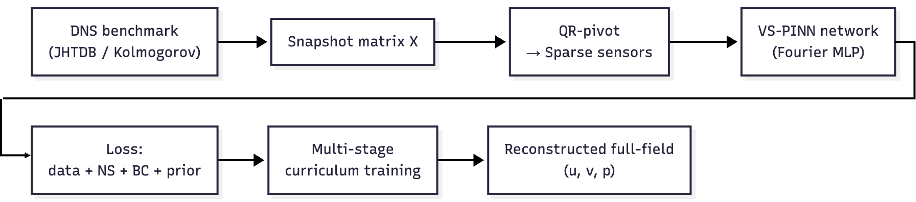
\includegraphics[width=1\linewidth]{result_figures/framework/framework.png}
    \caption{Sparse-sensor PINN reconstruction pipeline. Low-fidelity simulations (e.g., RANS or coarse LES) generate snapshots for QR-pivot sensor selection. A Fourier-feature VS-PINN is then trained from sparse measurements with data, PDE, BC, and prior losses, and uses DNS/JHTDB only as a controllable surrogate for virtual sensing (optionally with synthetic noise) and for a posteriori evaluation. In deployment, DNS is replaced by real sensor data.}
    \label{fig:framework}
\end{figure}

\section{PINNs for Inverse Problems: Foundations}
\label{sec:pinns_foundations}

Physics-Informed Neural Networks (PINNs), introduced by Raissi et al.\ (2019)~\cite{Raissi2019JCP}, embed governing partial differential equations (PDEs) as soft constraints in a differentiable training objective. Unlike purely data-driven approaches, PINNs can leverage sparse measurements alongside physical laws to infer hidden fields or unknown parameters~\cite{Karniadakis2021NRP}. This thesis adopts PINNs primarily as an \emph{inverse} reconstruction tool: the goal is not to solve a forward PDE from complete IC/BC data, but to recover turbulent velocity and pressure fields from limited observations while enforcing incompressible Navier--Stokes constraints.
The residual/BC/autodiff implementation used throughout this thesis was sanity-checked on the lid-driven cavity validation benchmark summarized in Appendix~\ref{appendix:wang2023_repro} (inspired by~\cite{wang2023solutionmultiplicityeffectsdata}) prior to applying it to Kolmogorov flow and JHTDB channel-flow reconstructions.

\begin{table}[!htbp]
    \centering
    \caption{Foundational milestones in PINNs research.}
    \label{tab:pinns_foundations}
    \small
    \begin{tabularx}{\textwidth}{
        >{\raggedright\arraybackslash}p{2.8cm}
        c
        >{\raggedright\arraybackslash}p{2.6cm}
        X
    }
    \toprule
    \textbf{Reference} & \textbf{Year} & \textbf{Problem Type} & \textbf{Key Contribution} \\
    \midrule
    Raissi et al.~\cite{Raissi2019JCP} & 2019 & Forward/Inverse & Introduced PINNs framework; demonstrated PDE solution without mesh \\
    Raissi et al.~\cite{Raissi2020Science} & 2020 & Inverse & Hidden Fluid Mechanics (HFM): reconstructed velocity and pressure from flow visualization; identified unknown forcing \\
    Karniadakis et al.~\cite{Karniadakis2021NRP} & 2021 & Review & Comprehensive review of physics-informed ML; highlighted inverse problem advantages \\
    Cai et al.~\cite{Cai2021JFM} & 2021 & Inverse 3D & Reconstructed 3D experimental flows from tomographic Schlieren data \\
    Yang et al.~\cite{Yang2021JCP} & 2021 & Bayesian & B-PINNs: added uncertainty quantification via variational inference \\
    Tancik et al.~\cite{tancik2020fourierfeaturesletnetworks} & 2020 & Architecture & Fourier feature embeddings to overcome spectral bias in MLPs \\
    Psaros et al.~\cite{Psaros2023JCP} & 2023 & Multifidelity & Unified multifidelity framework combining low- and high-fidelity data \\
    \bottomrule
    \end{tabularx}
\end{table}
\FloatBarrier

\section{Stabilization Ingredients Beyond Vanilla PINNs}
\label{sec:pinns_stabilization}

A fundamental bottleneck in PINNs---particularly for turbulent flows---is the ill-conditioned, highly non-convex loss landscape introduced by competing terms (data misfit, PDE residuals, boundary conditions) and disparate scales across variables and their derivatives. Vanilla PINNs, which use standard architectures and first-order optimizers without adaptive weighting, often suffer from slow or failed convergence due to gradient pathologies~\cite{Wang2021JCP}. This thesis builds its implementation on a set of practical stabilization ingredients that have proven effective across recent PINN studies, and instantiates them concretely in the architecture and training setup (Sections~\ref{sec:network_arch}--\ref{sec:adaptive_weighting}).

\begin{table}[!htbp]
    \centering
    \caption{Optimization and stabilization techniques for PINNs.}
    \label{tab:pinns_optimization}
    \footnotesize
    \begin{tabularx}{\textwidth}{
        >{\raggedright\arraybackslash}p{3.2cm}
        >{\raggedright\arraybackslash}p{3.4cm}
        X
    }
    \toprule
    \textbf{Technique} & \textbf{Reference} & \textbf{Key Idea / Advantage} \\
    \midrule
    \multicolumn{3}{l}{\textit{Loss Balancing \& Adaptive Weighting}} \\
    \midrule
    Likelihood-based adaptive weighting & Wang et al.~\cite{Wang2024} & Allocates loss weights via (Gaussian) likelihood estimation to balance terms \\
    GradNorm & Chen et al.~\cite{Chen2018ICML} & Multi-task learning weights adjusted by gradient norms \\
    Learning Rate Annealing & Wang et al.~\cite{Wang2021JCP} & Progressively refines PDE residuals as data fit improves \\
    \midrule
    \multicolumn{3}{l}{\textit{Architecture \& Initialization}} \\
    \midrule
    Variable Scaling (VS-PINN) & Ko \& Park~\cite{Ko2025JCP} & Learns per-variable scale factors $\{s_k\}$ to normalize outputs adaptively \\
    Fourier Features & Tancik et al.~\cite{tancik2020fourierfeaturesletnetworks} & Random Fourier embeddings overcome spectral bias; capture high frequencies \\
    PirateNet & Wang et al.~\cite{Wang2024JMLR} & Residual adaptive blocks improve gradient flow in deep networks \\
    Random Weight Factorization (RWF) & Wang et al.~\cite{wang2022randomweightfactorizationimproves} & Factorizes weights to improve continuous representation learning \\
    \midrule
    \multicolumn{3}{l}{\textit{Optimization Algorithms}} \\
    \midrule
    Adam + L-BFGS (two-phase) & Kingma \& Ba~\cite{Kingma2015Adam}, Rathore et al.~\cite{rathore2024challengestrainingpinnsloss} & Adam warm-up explores landscape; L-BFGS exploits local curvature for fast convergence \\
    NysNewton-CG (NNCG) & Rathore et al.~\cite{rathore2024challengestrainingpinnsloss} & Scalable second-order method using Nyström approximation of Hessian \\
    SOAP Optimizer & Vyas et al.~\cite{Vyas2024SOAP} & Shampoo-like adaptive preconditioner; can be paired with L-BFGS for fine-tuning \\
    \midrule
    \multicolumn{3}{l}{\textit{Sampling \& Curriculum}} \\
    \midrule
    Causal Training & Wang et al.~\cite{WANG2024116813} & For time-dependent PDEs: weights early times more to respect causality \\
    Time-Windowing & Multiple & Localizes residuals to temporal subdomains; reduces stiffness \\
    Adaptive Collocation & Nabian et al.~\cite{Nabian2021CMAME} & Re-samples collocation points in high-residual regions \\
    \bottomrule
    \end{tabularx}
\end{table}
\FloatBarrier

In this work, we adopt (i) VS-PINN output scaling and Fourier feature embeddings in the network backbone (Section~\ref{sec:network_arch}), (ii) explicit loss balancing and adaptive weighting strategies (Section~\ref{sec:adaptive_weighting}), and (iii) a practical optimizer stack (SOAP, optionally followed by L-BFGS) to accelerate convergence under stiffness.

\section{Governing Equations with Source Term Identification}
\label{sec:governing_eq}
We consider the reconstruction of an incompressible turbulent flow field $\mathbf{u} = (u, v, w)^T$ and pressure $p$ in a spatiotemporal domain $\Omega \times [0, T]$. To account for potential modeling errors or unmodeled external forcing, we introduce a learnable source term $\mathbf{S} = (S_x, S_y, S_z)^T$, following the methodology of Hidden Fluid Mechanics~\cite{Raissi2020Science}.

The governing equations are given by the incompressible Navier--Stokes equations:
\begin{subequations}
\label{eq:ns_system}
\begin{align}
    \nabla \cdot \mathbf{u} &= 0, \label{eq:continuity} \\
    \frac{\partial \mathbf{u}}{\partial t} + (\mathbf{u} \cdot \nabla) \mathbf{u} &= -\frac{1}{\rho} \nabla p + \nu \nabla^2 \mathbf{u} + \mathbf{S}, \label{eq:momentum}
\end{align}
\end{subequations}
where $\rho$ is the fluid density and $\nu$ is the kinematic viscosity. The source term $\mathbf{S}$ allows the network to absorb residuals not explained by the standard laminar operator.

\section{Network Architecture and Variable Scaling}
\label{sec:network_arch}
The function mapping $(\mathbf{x}, t) \mapsto (\mathbf{u}, p, \mathbf{S})$ is approximated by a fully connected neural network.
\begin{figure}[htbp]
    \centering
    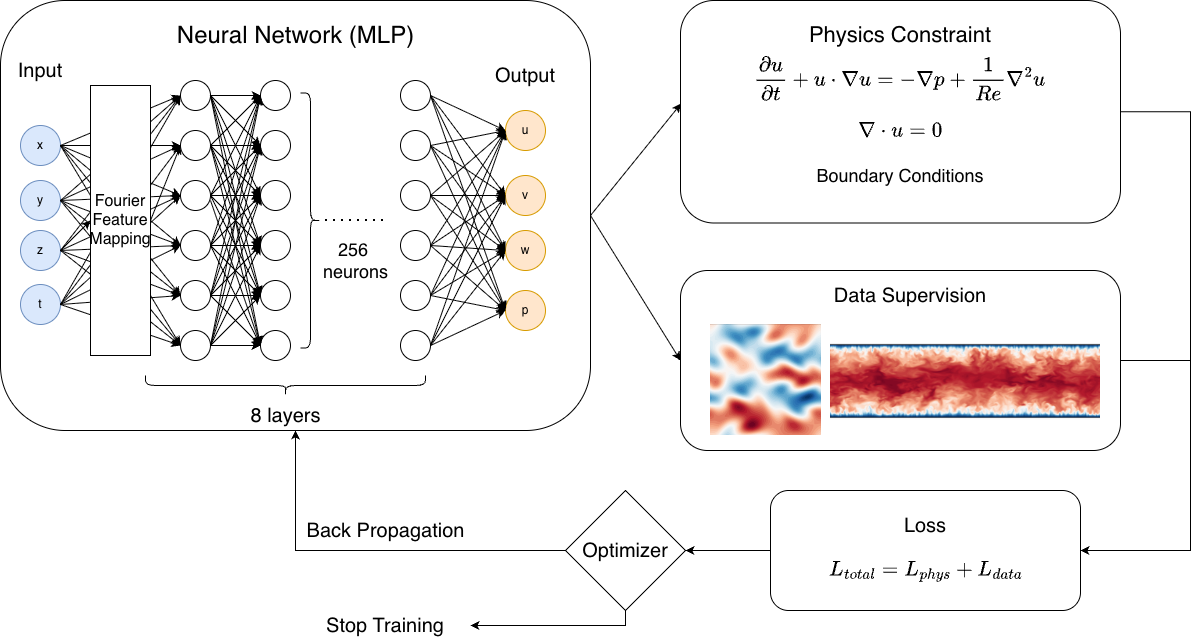
\includegraphics[width=\linewidth]{result_figures/framework/PINNs_structure.png}
    \caption{Schematic of the proposed VS-PINN architecture incorporating Fourier feature embeddings and anisotropic scaling factors.}
    \label{fig:network_arch}
\end{figure}

\subsection{Fourier Feature Embeddings}
Standard Multi-Layer Perceptrons (MLPs) are known to suffer from ``spectral bias,'' meaning they prioritize learning low-frequency functions and struggle to capture the high-frequency fluctuations characteristic of turbulence. To overcome this, we employ Fourier feature embeddings~\cite{tancik2020fourierfeaturesletnetworks} to map the input coordinates $\mathbf{x} \in \mathbb{R}^3$ into a higher-dimensional feature space.

The embedding function $\gamma(\mathbf{x})$ is defined as:
\begin{equation}
    \gamma(\mathbf{x}) = \left[ \cos(2\pi \mathbf{B} \mathbf{x}), \sin(2\pi \mathbf{B} \mathbf{x}) \right]^T,
\end{equation}
where $\mathbf{B} \in \mathbb{R}^{m \times 3}$ is a fixed weight matrix with entries sampled from a Gaussian distribution $\mathcal{N}(0, \sigma^2)$. By tuning the bandwidth parameter $\sigma$, we can control the frequency spectrum that the network is biased towards, enabling the PINN to resolve fine-scale vortices.

\subsection{Anisotropic Variable Scaling (VS-PINN)}
To mitigate the optimization stiffness arising from the domain geometry (e.g., channel flow), we employ the Variable-Scaling (VS-PINN) technique~\cite{Ko2025JCP}. The input coordinates are transformed via anisotropic scaling factors $\mathbf{N} = (N_x, N_y, N_z)$:
\begin{equation}
    (X, Y, Z) = (N_x x, N_y y, N_z z).
\end{equation}
Applying the chain rule, the spatial derivatives in the physical residual are scaled. For instance, the Laplacian in the momentum equation (Eq.~\eqref{eq:momentum}) becomes:
\begin{equation}
    \nabla^2 u = N_x^2 \frac{\partial^2 u}{\partial X^2} + N_y^2 \frac{\partial^2 u}{\partial Y^2} + N_z^2 \frac{\partial^2 u}{\partial Z^2}.
\end{equation}
Based on the physics of wall-bounded turbulence at $Re_\tau \approx 1000$, we determine the scaling factors $\mathbf{N} = (N_x, N_y, N_z)$.
In channel flows, flow structures exhibit strong anisotropy. The characteristic length scales in the wall-normal direction (determined by the viscous length scale $\delta_\nu$) are orders of magnitude smaller than the integral scales in the streamwise ($x$) and spanwise ($z$) directions; the JHTDB grid, for example, has $\Delta x^+ \approx 12.3$, $\Delta z^+ \approx 6.1$, and near-wall spacing $\Delta y_1^+ \ll 1$.
Standard isotropic neural networks struggle to resolve these sharp gradients near the wall ($y \approx \pm h$) while simultaneously covering the large domain extent.

To mitigate this spectral stiffness, we set $N_y = 12.0$ while keeping $N_x = N_z = 2.0$. 
This choice reflects the fact that near-wall gradients are roughly one order of magnitude larger in $y$ than in $x$ or $z$: by stretching the coordinate $y$ by a factor of 6 relative to $x$ and $z$, we effectively ``isotropicize'' the gradients seen by the network, balancing the back-propagated errors from wall-normal and streamwise derivatives without changing the underlying physical scales.

\subsection{Adaptive Residual Blocks and Random Weight Factorization}
\label{subsec:piratenet_components}
To further improve training stability and expressivity, recent work has proposed architectural components such as random weight factorization and residual connections. In this thesis, the MLP backbone supports two selectable block types: a standard feedforward (dense) block and a ResNet-style residual block (controlled by \texttt{model.block\_type}, e.g., \texttt{dense} vs.\ \texttt{resnet}). We use \texttt{block\_type=resnet} as the default setting in the reported experiments for consistency, and treat the ResNet-vs-dense comparison as a controlled ablation (holding the remaining settings fixed) to quantify the effect of residual connections.

\paragraph{Random Weight Factorization (RWF).}
Following the random weight factorization paradigm~\cite{wang2022randomweightfactorizationimproves}, each linear layer in the hidden MLP is parameterized as
\begin{equation}
    \mathbf{W} = \operatorname{diag}(\exp(\mathbf{s}))\,\mathbf{V},
\end{equation}
where $\mathbf{V}$ is a base weight matrix initialized using Xavier (Glorot) initialization~\cite{pmlr-v9-glorot10a} and $\mathbf{s}$ is a vector of learnable log-scale factors. The exponential scaling provides neuron-wise adaptive learning rates and can improve the optimization landscape for deep networks, particularly when combined with Fourier features~\cite{wang2022randomweightfactorizationimproves}.

\paragraph{ResNet-style Residual Blocks (optional).}
When \texttt{block\_type=resnet} is enabled, residual connections are implemented via learnable residual scaling in the form
\begin{equation}
    \mathbf{y} = \alpha\,f(\mathbf{x}) + (1-\alpha)\,\mathbf{x},
\end{equation}
where $f$ is a two-layer subnetwork and $\alpha$ is a trainable scalar initialized at $\alpha_{\text{init}}=0.0$. This interpolation formulation initializes the network as a shallow identity mapping ($\alpha \approx 0$) and gradually increases effective depth as training progresses, mitigating gradient pathologies in deep architectures~\cite{Wang2024JMLR, wang2025simulatingthreedimensionalturbulencephysicsinformed}.

\section{Sparse Sensor Placement via QR Pivoting}
\label{sec:sensor_placement}
Optimal sensor placement is critical for reconstructing turbulent fields from minimal data ($K \ll N$). While random sampling is commonly used, it often fails to capture the energetic structures of the flow. In this study, we adopt the QR decomposition with Column Pivoting (QRCP) strategy~\cite{Manohar2018PNAS}, which greedily selects measurement locations to improve the conditioning (i.e., reduce the condition number) of the sensing matrix. Figure~\ref{fig:qr_vs_random_sensors} illustrates the spatial distribution of QR-selected sensors compared to random placement on a 2D slice of the JHTDB channel flow, demonstrating the QR method's preference for near-wall regions with high velocity gradients.

In this thesis, low-fidelity fields play two distinct roles. First, low-fidelity snapshots are used to form the snapshot matrix $\mathbf{X}$ and to compute the QR pivots; the resulting pivot indices define the sparse sensor layout used for all subsequent reconstructions. Second, when enabled, the same low-fidelity fields serve as the target of the soft prior loss (Eq.~\eqref{eq:prior_loss}), evaluated at a set of prior collocation points; this role is treated as an explicit ablation knob and can be disabled independently of sensor design.

Let $\mathbf{X} \in \mathbb{R}^{N \times M}$ be the snapshot matrix containing $M$ flow realizations flattened into vectors of size $N$.
To ensure the selected sensors are robust for temporal reconstruction, the snapshots are sampled to span approximately one eddy turnover time, defined here as the flow-through time based on the streamwise domain length and bulk velocity, $T_e = L_x / U_b \approx 8\pi h / U_b \approx 25$ in the JHTDB scaling. This window captures diverse flow statistics rather than a single instantaneous state.
We first perform a Singular Value Decomposition (SVD) to extract the dominant spatial features:
\begin{equation}
    \mathbf{X} = \mathbf{U} \mathbf{\Sigma} \mathbf{V}^T,
\end{equation}
where $\mathbf{U}_r \in \mathbb{R}^{N \times r}$ represents the first $r$ Proper Orthogonal Decomposition (POD)~\cite{Sirovich1987QAM} modes. The goal is to find a selection matrix $\mathbf{C} \in \mathbb{R}^{K \times N}$ (consisting of canonical unit vectors) such that the condition number of the measured basis $\mathbf{C}\mathbf{U}_r$ is minimized.

This combinatorial problem is relaxed using QRCP applied to the transpose of the basis modes $\mathbf{U}_r^T$:
\begin{equation}
    \mathbf{U}_r^T \mathbf{P} = \mathbf{Q} \mathbf{R},
\end{equation}
where $\mathbf{P}$ is a permutation matrix, $\mathbf{Q}$ is unitary, and $\mathbf{R}$ is upper triangular with decreasing diagonal entries. The pivot indices in $\mathbf{P}$ correspond to the grid points that capture the largest volume in the feature space. We select the first $K$ pivots as our sensor locations $\mathcal{S}$, ensuring the measurements are optimally aligned with the flow's principal components.

\section{Loss Function Formulation}
\label{sec:loss_function}
The total loss function $\mathcal{L}_{\text{total}}$ is a weighted sum of five components: data consistency, physics residuals (momentum + continuity), boundary constraints (wall + periodic), low-fidelity prior consistency, and source-term regularization.
\begin{equation}
    \label{eq:total_loss}
    \mathcal{L}_{\text{total}} =
    w_{\text{data}}\mathcal{L}_{\text{data}}
    + \mathcal{L}_{\text{pde}}
    + \mathcal{L}_{\text{bc}}
    + w_{\text{prior}}\mathcal{L}_{\text{prior}}
    + \mathcal{L}_{\text{reg}}.
\end{equation}

\paragraph{Notation--configuration mapping.}
To avoid ambiguity, the weights used throughout this thesis correspond directly to the configuration keys reported in Appendix~\ref{appendix:configs}:
$w_{\text{data}} \leftrightarrow \text{\texttt{losses.data\_weight}}$,
$w_{\text{mom},k} \leftrightarrow \text{\texttt{losses.momentum\_\{x,y,z\}\_weight}}$,
$w_{\text{cont}} \leftrightarrow \text{\texttt{losses.continuity\_weight}}$ (or legacy \texttt{losses.div\_weight}),
$w_{\text{wall}} \leftrightarrow \text{\texttt{losses.wall\_constraint\_weight}}$,
$w_{\text{per}} \leftrightarrow \text{\texttt{losses.periodicity\_weight}}$,
$w_{\text{prior}} \leftrightarrow \text{\texttt{losses.prior\_weight}}$.

Training the PINN is therefore an optimization problem over the network parameters $\theta$:
\begin{equation}
    \theta^{*} = \arg\min_{\theta}\, \mathcal{L}_{\text{total}}(\theta),
\end{equation}
which is typically solved using gradient-based optimizers (e.g., Adam~\cite{Kingma2015Adam} and quasi-Newton methods). Conceptually, this can be viewed as navigating a high-dimensional \emph{loss landscape} and seeking a low-loss minimum that balances data fit and physics constraints (Figure~\ref{fig:loss_landscape}). In practice, due to non-convexity, convergence to the global minimum is not guaranteed; the figure should be interpreted as an illustrative schematic of the optimization objective.

\begin{figure}[htbp]
    \centering
    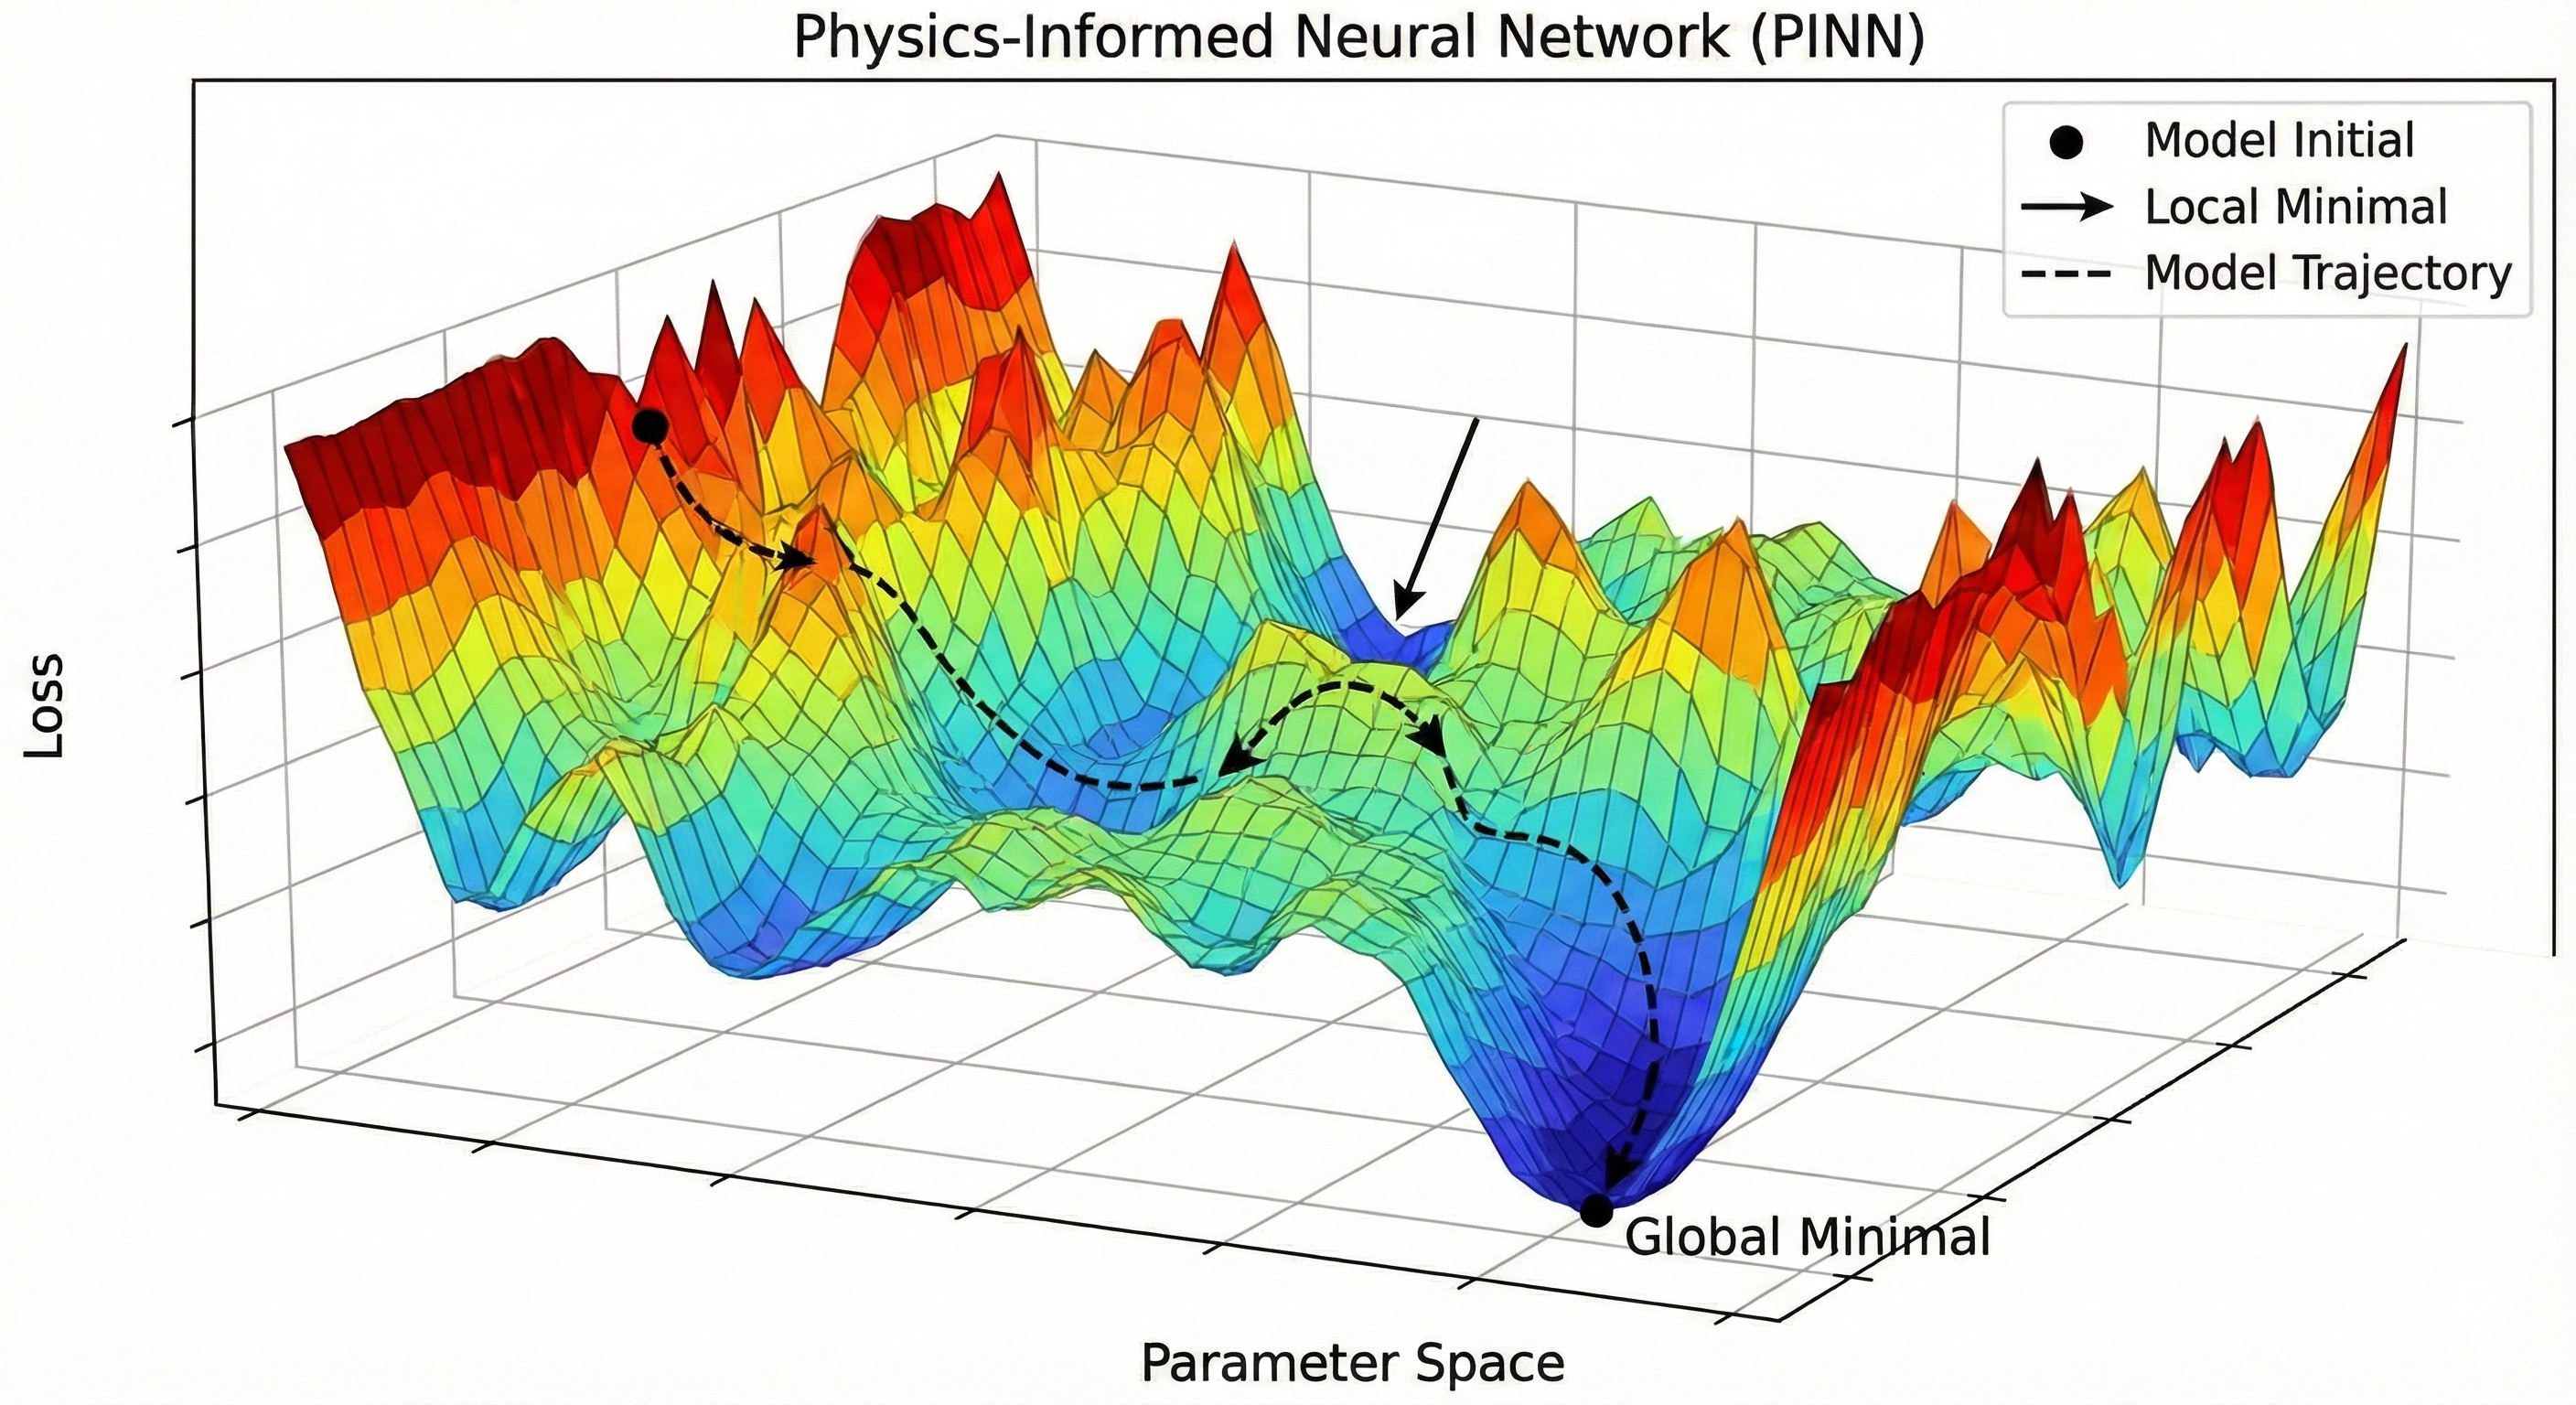
\includegraphics[width=0.95\linewidth]{result_figures/framework/loss_space.png}
    \caption{Schematic illustration of PINN training as optimization in parameter space: the optimizer follows a trajectory that reduces the composite loss and ideally approaches a low-loss basin. The ``global minimum'' is an idealized concept for intuition; practical training on non-convex loss surfaces typically converges to local or flat minima that yield acceptable physics-consistent reconstructions.}
    \label{fig:loss_landscape}
\end{figure}

\subsection{Data Consistency Loss}
The data loss ensures the reconstruction matches the sparse sensor measurements $\mathcal{D} = \{(\mathbf{x}_i, t_i, \mathbf{u}_i^{\text{obs}})\}_{i=1}^{N_{\text{sensor}}}$. To handle potential measurement noise, we employ a noise-weighted Mean Squared Error (MSE):
\begin{equation}
    \mathcal{L}_{\text{data}} = \frac{1}{N_{\text{sensor}}} \sum_{i=1}^{N_{\text{sensor}}} \sum_{\phi \in \{u,v,w\}} \frac{1}{\sigma_i^2 + \epsilon} \left\| \phi_{\text{pred}}(\mathbf{x}_i) - \phi_{\text{obs}}(\mathbf{x}_i) \right\|^2,
\end{equation}
where $\sigma_i$ represents the observation noise standard deviation and $\epsilon=10^{-8}$ is a stability term. In this study, the sparse sensors are assumed to measure only the three velocity components; extending the formulation to include pressure observations is straightforward when such data are available.

\subsection{Evaluation Metrics}
For quantitative evaluation, we report the relative $L_2$ error of each field $\phi \in \{u,v,w,p\}$ as
\begin{equation}
    \label{eq:rel_l2_def}
    \mathrm{rel}\,L_2(\phi) = \frac{\|\phi_{\text{pred}} - \phi_{\text{DNS}}\|_2}{\|\phi_{\text{DNS}}\|_2},
\end{equation}
where the norms are computed over the spatial grid used for comparison. When reported in percent, we multiply Eq.~\eqref{eq:rel_l2_def} by $100$. Unless otherwise stated, all relative $L_2$ values in this thesis follow this definition. For pressure, we subtract the spatial mean from both prediction and DNS before computing Eq.~\eqref{eq:rel_l2_def} to fix the gauge; we additionally interpret pressure-gradient errors using dedicated metrics as discussed in the evaluation report.

\subsection{Physics Residual Loss}
The physics loss enforces the governing equations (Eq.~\ref{eq:ns_system}) at $N_{\text{pde}}$ collocation points.
To resolve the sharp gradients in the boundary layer, we employ a \textbf{stratified sampling strategy} where the density of collocation points is higher near the walls ($y \approx \pm h$), following a hyperbolic tangent distribution. Recent work has also proposed QR-DEIM-based adaptive collocation strategies tailored for PINNs~\cite{celaya2025adaptive}; here we opt for a simpler wall-focused stratified sampling scheme that is well-suited to channel-flow geometries.
It comprises the momentum residuals ($\mathcal{L}_{\text{mom},k}$) and the continuity residual ($\mathcal{L}_{\text{cont}}$), calculated via automatic differentiation~\cite{Raissi2019JCP} and weighted by $(w_{\text{mom},k}, w_{\text{cont}})$:
\begin{equation}
    \label{eq:pde_loss}
    \mathcal{L}_{\text{pde}} = \frac{1}{N_{\text{pde}}} \sum_{j=1}^{N_{\text{pde}}} \left( \sum_{k \in \{x,y,z\}} w_{\text{mom}, k}\|\mathcal{R}_{\text{mom}, k}(\mathbf{x}_j)\|^2 + w_{\text{cont}}\|\nabla \cdot \mathbf{u}(\mathbf{x}_j)\|^2 \right).
\end{equation}

\subsection{Boundary Condition Loss}
Boundary constraints are explicitly enforced via penalty terms.
\paragraph{No-Slip Wall:} On the channel walls ($y = \pm h$), we enforce zero velocity:
\begin{equation}
    \mathcal{L}_{\text{wall}} = \frac{1}{N_{\text{wall}}} \sum_{\mathbf{x} \in \Gamma_{\text{wall}}} \|\mathbf{u}(\mathbf{x})\|^2.
\end{equation}
\paragraph{Periodic Boundary:} Periodic conditions are applied in the streamwise ($x$) and spanwise ($z$) directions:
\begin{equation}
    \mathcal{L}_{\text{periodic}} = \frac{1}{N_{\text{bc}}} \sum_{j=1}^{N_{\text{bc}}} \left\| \mathbf{u}(x_{\min}, \dots)_j - \mathbf{u}(x_{\max}, \dots)_j \right\|^2.
\end{equation}
In practice, we enforce periodicity explicitly on the velocity components; the pressure field is constrained through the incompressible Navier--Stokes residual together with an imposed constant streamwise pressure gradient and is interpreted up to an additive constant (pressure gauge).
\begin{equation}
    \mathcal{L}_{\text{bc}} = w_{\text{wall}}\mathcal{L}_{\text{wall}} + w_{\text{per}}\mathcal{L}_{\text{periodic}}.
\end{equation}

\subsection{Pressure Handling and Gauge Choice}
For channel flow, the driving mechanism is a constant mean pressure gradient in the streamwise direction. In the VS-PINN channel-flow formulation, we explicitly include a constant forcing term $dP/dx$ in the $x$-momentum equation while predicting a pressure field $p(\mathbf{x})$ that represents fluctuations consistent with this mean gradient. Since incompressible pressure is defined only up to an additive constant, we fix the gauge implicitly by penalizing the pressure in a small reference region and, in all post-processing, subtract the spatial mean from both DNS and reconstructed fields before visualization or error computation. Quantitative pressure metrics therefore focus on pressure gradients and gauge-fixed fluctuations rather than absolute pressure levels.

\subsection{Prior Consistency Loss (Low-Fidelity)}
To address the ill-posedness of sparse reconstruction, we incorporate low-fidelity simulation data (RANS/LES), denoted as $\phi^{\text{LF}}$, as a soft prior~\cite{Psaros2023JCP}. Unlike hard constraints, this loss penalizes deviations from the prior only when data or physics do not dictate otherwise:
\begin{equation}
    \label{eq:prior_loss}
    \mathcal{L}_{\text{prior}} = \frac{1}{N_{\text{prior}}} \sum_{i=1}^{N_{\text{prior}}} \sum_{\phi \in \{u,v,w\}} \left\| \phi^{\text{HF}}(\mathbf{x}_i) - \phi^{\text{LF}}(\mathbf{x}_i) \right\|^2.
\end{equation}
Here $N_{\text{prior}}$ denotes the number of collocation points at which the prior loss is evaluated. This term acts as a \emph{soft point-wise regularizer} that biases the reconstruction toward a physically plausible low-frequency/mean state in regions void of sensors, while allowing sparse measurements and physics residuals to correct local deviations~\cite{Xu2022}.
Unless otherwise stated, the low-fidelity field used in Eq.~\eqref{eq:prior_loss} is the same low-fidelity dataset used to design the QR-pivot sensor layout (Section~\ref{sec:sensor_placement}); sensor design and the prior-loss term are treated as separable components and can be ablated independently.
In the channel-flow experiments, we intentionally exclude pressure from this point-wise prior and constrain it only through the momentum equations and the imposed mean pressure gradient to avoid conflating the arbitrary pressure gauge with the low-fidelity mean field.

\subsection{Synergy between Source Term and RANS Prior}
A critical challenge in this framework is distinguishing the roles of the learned source term $\mathbf{S}$ (Eq.~\ref{eq:momentum}) and the RANS prior (Eq.~\ref{eq:prior_loss}). 
Using both simultaneously requires careful justification to prevent overfitting.

\paragraph{Complementary Roles:}
The RANS prior $\mathbf{u}_{\text{RANS}}$ provides a ``global guide'' for the mean flow structure, particularly in regions void of sensors. However, RANS models inherently suffer from structural biases (e.g., isotropy assumptions in $k-\epsilon$) and cannot capture instantaneous turbulent fluctuations.
The learnable source term $\mathbf{S}$, on the other hand, is designed to absorb these specific discrepancies:
\begin{enumerate}
    \item \textbf{Model Bias Correction:} $\mathbf{S}$ compensates for the mismatch between the RANS-predicted mean field and the instantaneous DNS reality.
    \item \textbf{Instantaneous Dynamics:} Since NS equations are applied to instantaneous fields, $\mathbf{S}$ captures the unmodeled forcing or transient features that the steady RANS prior misses.
\end{enumerate}

\paragraph{Prevention of Trivial Solutions:}
To ensure the network respects the physics (Navier--Stokes) and does not simply reproduce the RANS solution while using a large source term to artificially reduce the PDE residual, we impose $L_1$ regularization on $\mathbf{S}$ (Eq.~\ref{eq:reg_loss}).
This enforces sparsity, compelling the network to explain the flow dynamics via the standard NS operators ($\mathbf{u} \cdot \nabla \mathbf{u} + \nabla p - \nu \nabla^2 \mathbf{u}$) as much as possible, utilizing $\mathbf{S}$ only when the physical residual is irreducible due to data/prior mismatch.

\subsection{Source Term Regularization}
To prevent the learned source term $\mathbf{S}$ from overfitting or absorbing physical dynamics, we apply $L_1$ regularization to enforce sparsity, inspired by techniques in sparse identification of nonlinear dynamics~\cite{Raissi2020Science}:
\begin{equation}
    \label{eq:reg_loss}
    \mathcal{L}_{\text{reg}} = \lambda_{\text{reg}} \frac{1}{N_{\text{pde}}} \sum_{i=1}^{N_{\text{pde}}} \left( |S_x|_i + |S_y|_i + |S_z|_i \right),
\end{equation}
with $\lambda_{\text{reg}}$ typically set between $10^{-6}$ and $10^{-4}$.

\section{Adaptive Weighting Strategy}
\label{sec:adaptive_weighting}
Balancing the competing loss terms is a central practical challenge in PINN training. The literature includes automated weighting mechanisms such as causal weighting for time-dependent problems~\cite{WANG2024116813} and gradient-norm-based balancing (e.g., GradNorm-style approaches)~\cite{Ko2025JCP, 10.1063/5.0180770}. In this thesis, to keep the experimental protocol interpretable and reproducible, we primarily use explicitly specified loss weights (fixed weights in the vanilla baseline and a staged curriculum in the soft prior variant) rather than enabling fully automated weight adaptation.

\begin{algorithm}[t]
  \SetAlgoLined
  \caption{Proposed Framework: Sparse Turbulence Reconstruction}
  \label{alg:reconstruction}
  
  \KwIn{Sparse observations $\mathcal{D} = \{(\mathbf{x}_i, \mathbf{u}_i)\}_{i=1}^K$; Low-fidelity prior $\mathbf{u}_{\text{prior}}$; Domain $\Omega$}
  \KwOut{Reconstructed high-fidelity fields $\hat{\mathbf{u}}$}

  \tcp{1. Sensor Placement}
  Compute POD basis from snapshot matrix $\mathbf{X}$\;
  Select sensor locations $\mathcal{S}$ via QR-pivoting on basis modes\;

  \tcp{2. Initialization}
  Initialize Neural Network $f_\theta$ with Fourier features\;
  Set anisotropic scaling factors $(N_x, N_y, N_z) = (2, 12, 2)$ based on domain aspect ratio\;
  
  \tcp{3. Training Loop}
  \For{$\text{epoch} = 1$ \KwTo $N_{\text{epochs}}$}{
      Compute $\mathcal{L}_{\text{data}}$ on sparse sensors $\mathcal{S}$\;
      Compute $\mathcal{L}_{\text{pde}}$ (NS residuals + Source Term regularization)\;
      Compute $\mathcal{L}_{\text{prior}}$ (Soft constraint to $\mathbf{u}_{\text{prior}}$)\;
      
      Update weights using a fixed schedule (or a staged curriculum, if enabled)\;
      Optimize $\theta$ using SOAP (optionally followed by L-BFGS for fine-tuning)\;
  }
  \Return{$\hat{\mathbf{u}}$}
\end{algorithm}

\section{Low-Fidelity Data Generation (RANS)}
\label{sec:rans_setup}
To address the ill-posedness of reconstruction from sparse measurements ($K=100$), we utilize low-fidelity simulation data as a soft prior. In this thesis, the prior enters the inverse problem through a \emph{soft point-wise} consistency loss (Eq.~\eqref{eq:prior_loss}) with explicit weight scheduling, rather than as a hard point-wise target.
The Reynolds-Averaged Navier--Stokes (RANS) equations are solved using the commercial CFD solver ANSYS Fluent to obtain the mean flow fields.

\subsection{Simulation Setup}
The computational domain matches the JHTDB channel flow dimensions ($8\pi h \times 2h \times 3\pi h$).
To emulate a realistic engineering scenario where DNS-level resolution is unavailable, we employ a significantly coarser grid compared to the DNS baseline.
The simulation is governed by the steady-state incompressible RANS equations closed with the $k$-$\omega$ SST turbulence model, which provides improved near-wall prediction capability compared to the standard $k$-$\epsilon$ model for wall-bounded flows~\cite{Menter1994}.
\textbf{Note that all flow variables are non-dimensionalized by the channel half-height $h$ and the bulk velocity $U_{bulk}$ consistent with the JHTDB format.}

Table~\ref{tab:fluent_rans_setup} summarizes the complete Fluent RANS simulation parameters used in this work.

\begin{table}[htbp]
    \centering
    \caption{ANSYS Fluent RANS simulation configuration for channel flow at $Re_\tau \approx 1000$.}
    \label{tab:fluent_rans_setup}
    \begin{tabular}{ll}
    \toprule
    \textbf{Parameter} & \textbf{Value / Setting} \\
    \midrule
    \multicolumn{2}{c}{\textbf{Solver Configuration}} \\
    Solver Type & Pressure-Based \\
    Time Mode & Steady State \\
    Velocity Formulation & Absolute \\
    Turbulence Model & $k$-$\omega$ SST \\
    Spatial Discretization & Second Order (all variables) \\
    Gradient Calculation & Least Squares Cell Based \\
    Pressure-Velocity Coupling & SIMPLE Scheme \\
    Convergence Acceleration & Pseudo Transient \\
    \midrule
    \multicolumn{2}{c}{\textbf{Computational Grid}} \\
    Grid Resolution $(N_x \times N_y \times N_z)$ & $251 \times 20 \times 94$ \\
    Total Cell Count & $471,880$ \\
    First Layer Height $\Delta y_1$ & $0.03$ (non-dimensional) \\
    Wall-Normal $y^+$ at First Cell & $\approx 30$ \\
    Streamwise/Spanwise Distribution & Uniform \\
    Wall-Normal Distribution & Wall-refined (geometric progression) \\
    \midrule
    \multicolumn{2}{c}{\textbf{Physical Properties (Non-dimensional)}} \\
    Density $\rho$ & $1.0$ \\
    Kinematic Viscosity $\nu$ & $5 \times 10^{-5}$ \\
    Mean Pressure Gradient $dP/dx$ & $+0.0025$ \\
    \midrule
    \multicolumn{2}{c}{\textbf{Domain Geometry}} \\
    Streamwise Length $L_x$ & $[0.050, 25.083]$ ($\approx 8\pi h$) \\
    Wall-Normal Height $L_y$ & $[0.050, 1.950]$ ($\approx 2h$) \\
    Spanwise Width $L_z$ & $[0.050, 9.375]$ ($\approx 3\pi h$) \\
    \midrule
    \multicolumn{2}{c}{\textbf{Convergence Criteria}} \\
    Residual Target & $10^{-6}$ (all variables) \\
    Maximum Iterations & $5000$--$10000$ \\
    Reporting Interval & $100$ iterations \\
    \bottomrule
    \end{tabular}
\end{table}

\paragraph{Model Fidelity Characteristics.}
The resulting RANS solution yields an estimated friction Reynolds number $Re_\tau^{\text{RANS}} \approx 1344$, which is approximately $34\%$ higher than the DNS target $Re_\tau \approx 1000$ (see Section~\ref{sec:jhtdb_data}). This over-prediction is a known characteristic of the $k$-$\omega$ SST model, which typically over-estimates turbulent kinetic energy by $30$--$40\%$ in wall-bounded flows~\cite{Menter1994}. Despite this systematic bias, the RANS field captures the correct qualitative flow topology (mean velocity profile, turbulence intensity distribution) and can serve as an effective \emph{soft point-wise} prior regularizer when coupled with appropriate weight scheduling and the learnable source term $\mathbf{S}$ to absorb model-form errors.
Figure~\ref{fig:rans_dns_velocity_profiles} presents a quantitative comparison of the RANS and DNS velocity profiles, revealing an overall $L_2$ relative error of $33.24\%$ with peak discrepancies exceeding $98\%$ in the near-wall region. This substantial error---characteristic of RANS turbulence closures in high-Reynolds-number wall-bounded flows---underscores the necessity of sparse high-fidelity measurements to anchor the reconstruction, while the RANS field provides global regularization to mitigate ill-posedness in under-sampled regions.

\paragraph{Coordinate System Note.}
An important practical detail is that the RANS simulation uses a coordinate system with $y \in [0.050, 1.950]$ (bottom wall at $y \approx 0$), whereas the JHTDB DNS reference uses $y \in [-1, 1]$ (channel centerline at $y = 0$). During PINN training, the RANS prior values are transformed to the DNS coordinate frame via $y_{\text{DNS}} = y_{\text{RANS}} - 1.0$ before being applied in the prior consistency loss (Eq.~\ref{eq:prior_loss}). This transformation ensures that the soft prior is spatially aligned with the high-fidelity DNS reference and the sensor measurements.

\subsection{Boundary Conditions}
Boundary conditions are set to match the friction Reynolds number $Re_\tau \approx 1000$ of the JHTDB benchmark:
\begin{itemize}
    \item \textbf{Streamwise ($x$) and Spanwise ($z$):} Periodic boundary conditions are applied to mimic the infinite channel assumption.
    \item \textbf{Wall-normal ($y$):} No-slip conditions ($u=v=w=0$) are enforced at the top and bottom walls ($y = \pm h$).
    \item \textbf{Driving Force:} A constant pressure gradient is applied in the streamwise direction to maintain the target flow rate.
\end{itemize}
The resulting steady-state velocity field $\mathbf{u}_{\text{RANS}}$ serves as the input for the prior consistency loss ($\mathcal{L}_{\text{prior}}$) defined in Section \ref{sec:loss_function}.

\subsection{Data Alignment and Interpolation}
A practical challenge arises from the resolution mismatch between the coarse RANS grid and the continuous domain of the PINN framework. The RANS simulation provides discrete field values $\mathbf{u}_{\text{RANS}}$ on a finite volume mesh $\mathcal{M}_{\text{coarse}}$, whereas the physics-informed loss (Eq.~\ref{eq:pde_loss}) and prior loss (Eq.~\ref{eq:prior_loss}) are evaluated at arbitrary collocation points $\{\mathbf{x}_p\}$ sampled continuously within the domain.

To bridge this gap, we employ \textbf{trilinear interpolation} to map the discrete RANS solution onto the query coordinates of the PINN training batch. For any collocation point $\mathbf{x}_p = (x, y, z)$, the prior value $\mathbf{u}_{\text{RANS}}(\mathbf{x}_p)$ is computed by interpolating from the eight nearest cell centers in the coarse mesh. This approach ensures that the soft prior provides a smooth, differentiable guidance field without imposing the artificial discretization artifacts of the low-fidelity grid onto the high-fidelity reconstruction.

Although trilinear interpolation may introduce local smoothing effects---particularly in near-wall regions with high gradients---this is acceptable within the proposed framework.
Since the RANS field serves only as a \emph{soft prior} (statistical guidance) rather than a hard constraint, and the learnable source term $\mathbf{S}$ is explicitly designed to compensate for model-form discrepancies and recover high-frequency details, the potential smoothing from interpolation does not compromise the final reconstruction accuracy.

\begin{figure}[htbp]
    \centering
    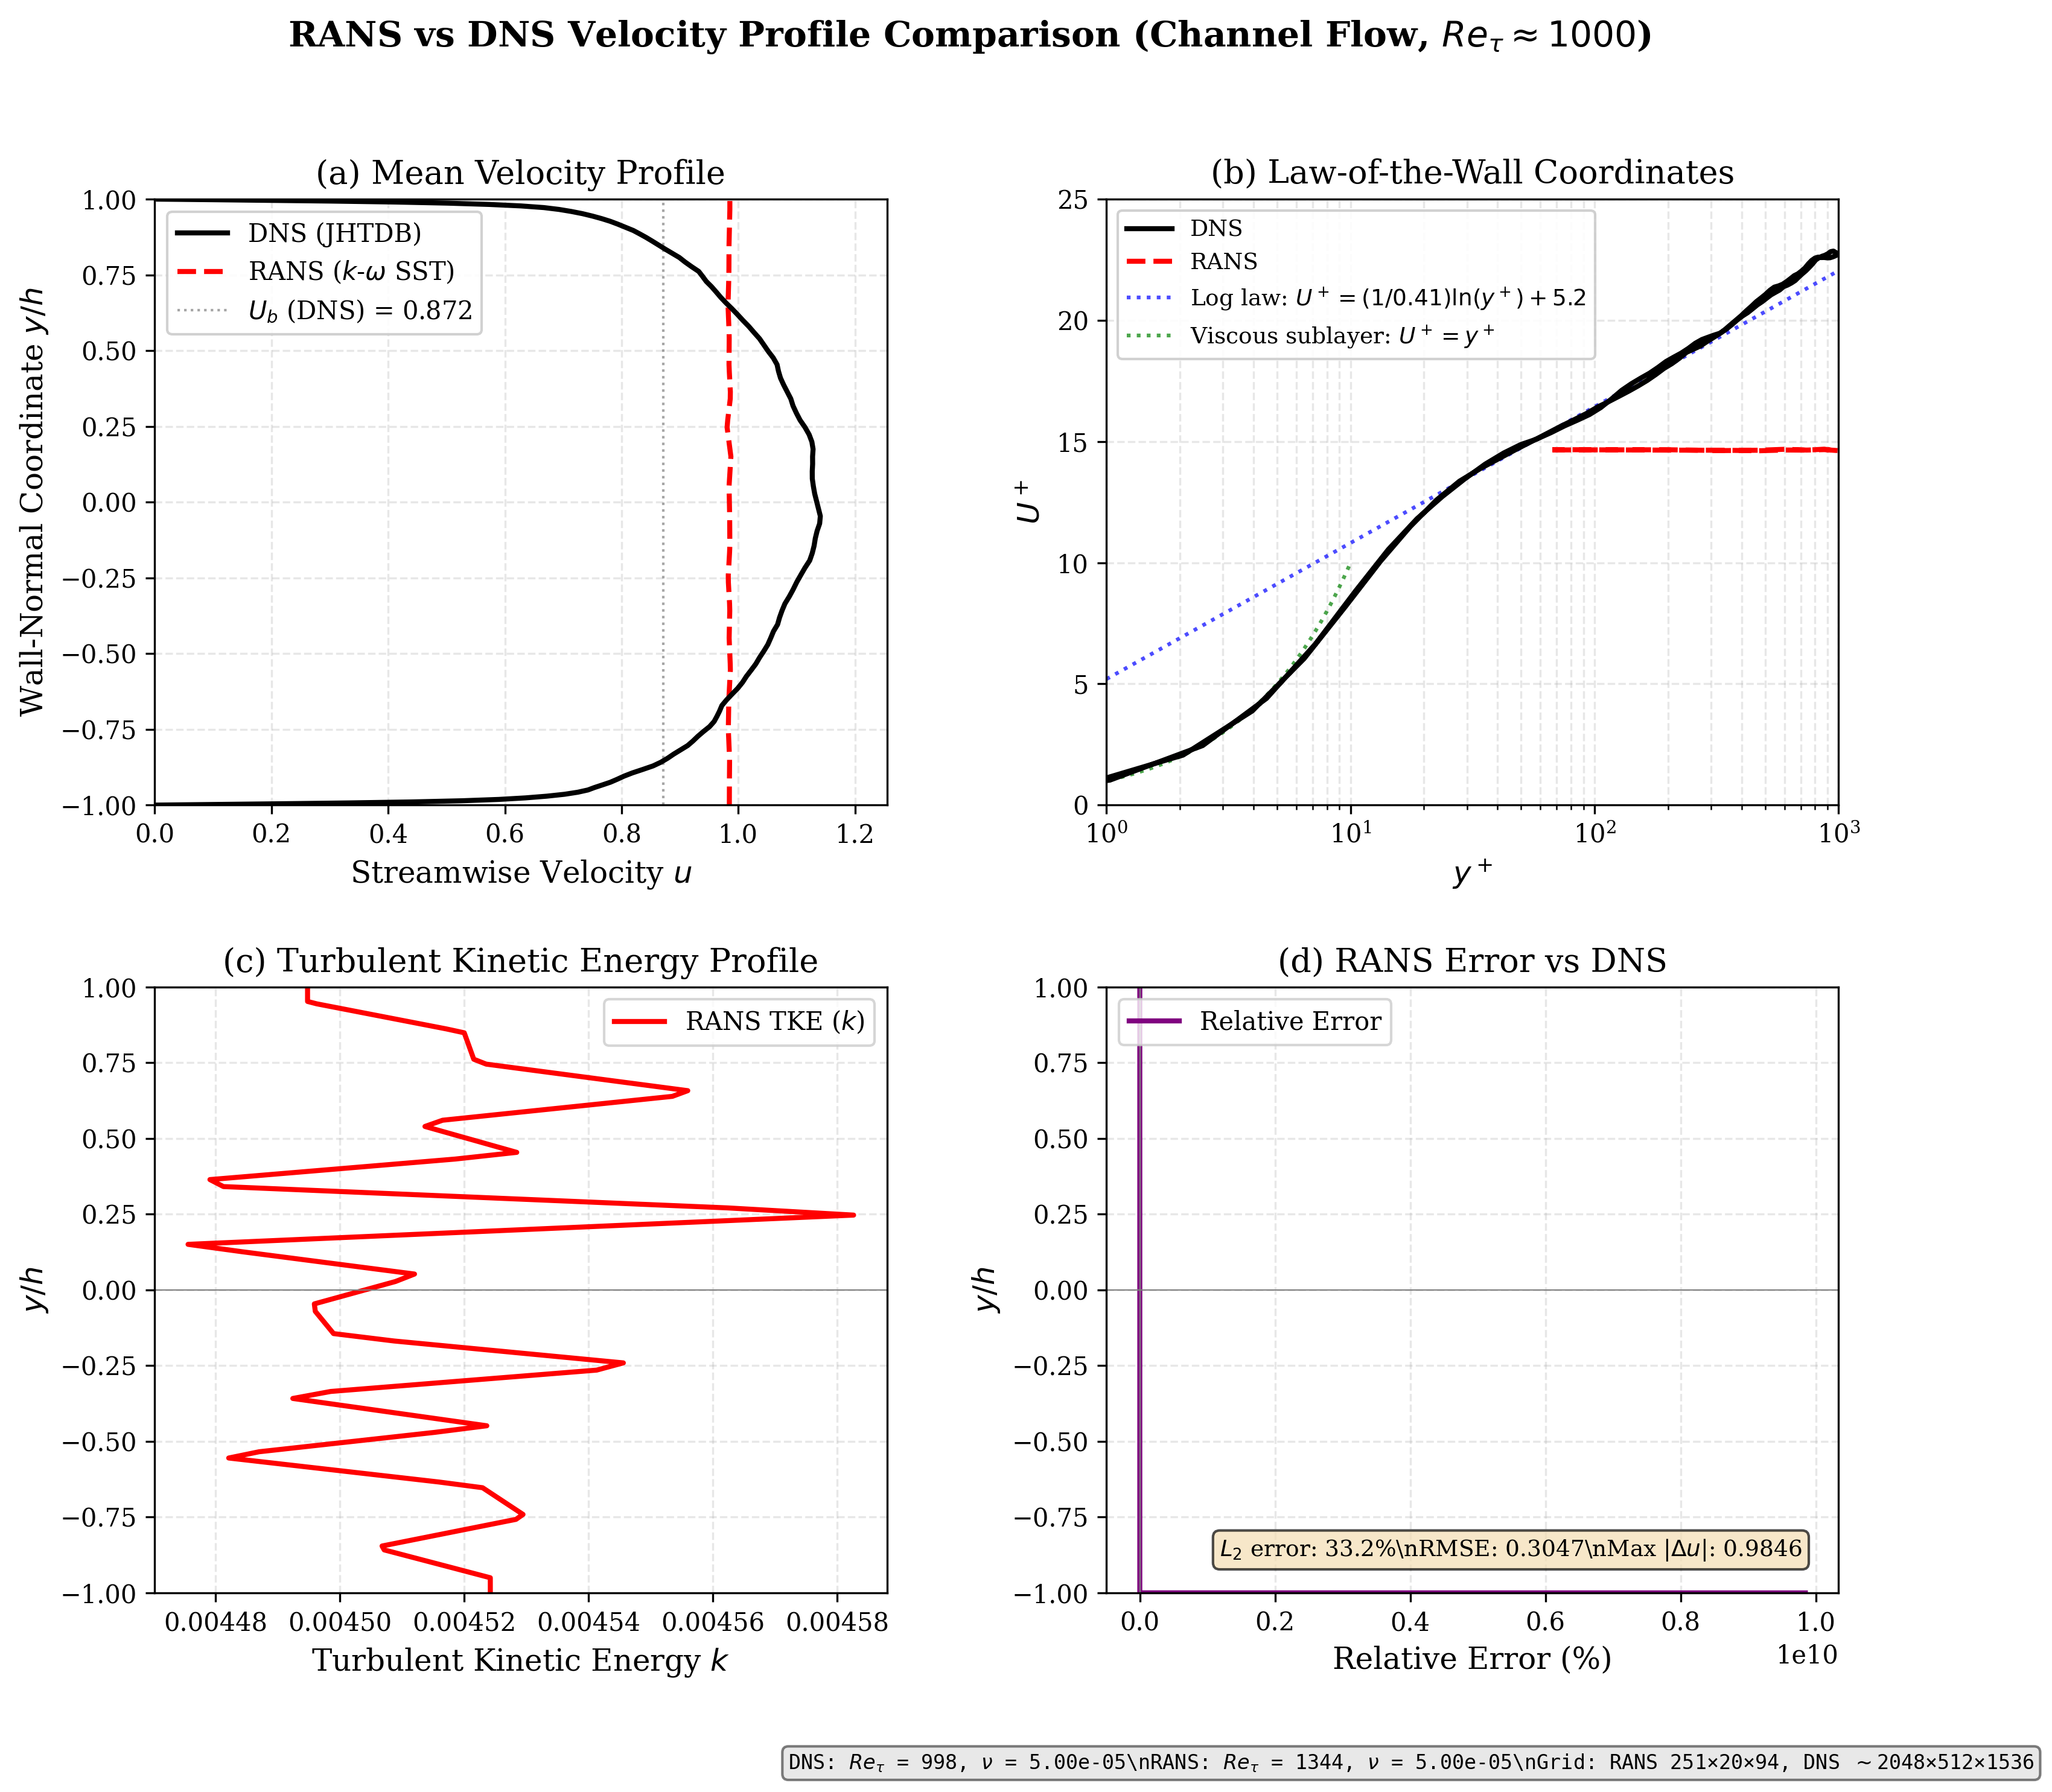
\includegraphics[width=0.95\textwidth]{result_figures/channel_flow/rans_dns_velocity_profiles.png}
    \caption{%
        \textbf{RANS ($k$-$\omega$ SST) vs.\ DNS (JHTDB) velocity profile comparison.}
        \textbf{(a)} Mean streamwise velocity profile in outer units, showing RANS over-prediction of centerline velocity due to excessive turbulent kinetic energy.
        \textbf{(b)} Law-of-the-wall comparison in wall units ($U^+$ vs.\ $y^+$), with logarithmic layer reference line $U^+ = \frac{1}{\kappa}\ln y^+ + B$ ($\kappa = 0.41$, $B = 5.0$). RANS captures the log-law slope but over-estimates wake region velocity.
        \textbf{(c)} Turbulent kinetic energy profile from RANS, illustrating the model's tendency to over-predict TKE by 30--40\% compared to DNS (not shown due to unavailability of instantaneous fluctuations in mean-field RANS).
        \textbf{(d)} Pointwise relative error $|u_{\text{RANS}} - u_{\text{DNS}}|/u_{\text{DNS}}$ across the channel height, with statistical metrics: $L_2$ relative error = 33.24\%, RMSE = 0.305, maximum error = 98.97\% (near wall). 
        The substantial discrepancy---particularly in the near-wall and wake regions---motivates the use of RANS exclusively as a \emph{soft prior} rather than a hard constraint, with sparse DNS sensor measurements ($K \leq 100$) providing high-fidelity anchoring.
    }
    \label{fig:rans_dns_velocity_profiles}
\end{figure}

\subsection{Low-Fidelity Prior: Leith Turbulence Model for 2D Kolmogorov Flow}
\label{sec:kolmogorov_rans_setup}
In contrast to the 3D channel-flow RANS prior described above, the 2D Kolmogorov flow validation experiments require a turbulence closure specifically designed for two-dimensional flows. Standard RANS models (e.g., $k$--$\varepsilon$, $k$--$\omega$ SST) are fundamentally inappropriate for 2D turbulence because they assume a forward energy cascade (large scales $\to$ small scales), whereas 2D turbulence exhibits an \emph{inverse} energy cascade (small scales $\to$ large scales) alongside a forward enstrophy cascade~\cite{Boffetta2012ARFM}. Therefore, we employ the \textbf{Leith turbulence model}~\cite{Leith1996PhysFluids}, which estimates the eddy viscosity based on local vorticity gradients rather than solving additional transport equations.

The Leith model augments the incompressible Navier--Stokes equations for a doubly-periodic domain $[0, 2\pi] \times [0, 2\pi]$ with a uniform sinusoidal body force $\mathbf{f} = A \sin(k_f y) \hat{\mathbf{e}}_y$:
\begin{align}
    \nabla \cdot \mathbf{u} &= 0, \\
    \frac{\partial \mathbf{u}}{\partial t} + \mathbf{u} \cdot \nabla \mathbf{u} &= -\frac{1}{\rho}\nabla p + \nabla \cdot \left[(\nu + \nu_t) \nabla \mathbf{u}\right] + \mathbf{f},
\end{align}
where the eddy viscosity is computed diagnostically from the vorticity field:
\begin{equation}
    \nu_t = (C_L \Delta)^3 |\nabla \omega|, \quad \omega = \frac{\partial v}{\partial x} - \frac{\partial u}{\partial y}.
\end{equation}
Here, $C_L \approx 0.2$ is the Leith constant, $\Delta = \sqrt{\Delta x \Delta y}$ is the grid spacing, and $|\nabla \omega| = \sqrt{(\partial \omega/\partial x)^2 + (\partial \omega/\partial y)^2}$ is the magnitude of the vorticity gradient. This vorticity-gradient-based closure naturally adapts to local flow structure without requiring additional transport equations, making it computationally efficient and physically consistent with 2D turbulence dynamics.

\paragraph{Solver Configuration.}
The Leith-model fields are generated using a pseudo-spectral (Fourier) solver with $2/3$-rule dealiasing implemented in Python on a uniform $128 \times 128$ Cartesian grid. Starting from random initial conditions or a coarse DNS field, the solver time-integrates the Leith-augmented Navier--Stokes equations using a semi-implicit Runge--Kutta scheme until the flow reaches a statistically stationary state. Periodic boundary conditions are enforced in both $x$ and $y$ directions. Each simulation is run for a total time $T_{\text{total}} = 100$ with a spinup period $T_{\text{spinup}} = 10$, and time-averaged snapshots are extracted from the statistically stationary regime. For the baseline validation case at $Re=50$ with $k_f=4$, forcing amplitude $A=1.0$, and Leith constant $C_L=0.2$, the time-averaged solution exhibits spatially varying eddy viscosity ($\nu_t$ ranging from 0.02 to 0.15) and captures approximately 56\% of the DNS kinetic energy. Table~\ref{tab:kolmogorov_rans_params} summarizes the key parameters.

\begin{table}[htbp]
    \centering
    \caption{Leith turbulence model parameters for 2D Kolmogorov flow at $Re=50$, $k_f=4$.}
    \label{tab:kolmogorov_rans_params}
    \begin{tabular}{ll}
    \toprule
    \textbf{Parameter} & \textbf{Value} \\
    \midrule
    \multicolumn{2}{c}{\textbf{Physical Configuration}} \\
    Reynolds number $Re$ & 50 \\
    Kinematic viscosity $\nu$ & 0.039374 \\
    Forcing wavenumber $k_f$ & 4 \\
    Forcing amplitude $A$ & 1.0 \\
    Domain size $(L_x, L_y)$ & $(2\pi, 2\pi)$ \\
    \midrule
    \multicolumn{2}{c}{\textbf{Computational Grid}} \\
    Grid resolution $(N_x \times N_y)$ & $128 \times 128$ \\
    Cell spacing $\Delta x = \Delta y$ & $2\pi/128 \approx 0.049$ \\
    Grid length scale $\Delta$ & $\sqrt{\Delta x \Delta y} \approx 0.049$ \\
    Total cells & 16,384 \\
    Boundary conditions & Periodic (both directions) \\
    \midrule
    \multicolumn{2}{c}{\textbf{Leith Turbulence Closure}} \\
    Leith constant $C_L$ & 0.20 (uniform across all $Re$) \\
    Eddy viscosity formula & $\nu_t = (C_L \Delta)^3 |\nabla \omega|$ \\
    Time-averaged $\langle \nu_t \rangle$ & $0.082 \pm 0.035$ \\
    Time-averaged kinetic energy & $0.56 \times E_{\text{DNS}}$ \\
    \midrule
    \multicolumn{2}{c}{\textbf{Time Integration}} \\
    Time step $\Delta t$ & 0.005 \\
    Total integration time $T_{\text{total}}$ & 100 \\
    Spinup time $T_{\text{spinup}}$ & 10 \\
    Time-averaging window & $[10, 100]$ \\
    \bottomrule
    \end{tabular}
\end{table}

\paragraph{Model Fidelity and Intended Role.}
The Leith model provides a physically consistent low-fidelity baseline for 2D Kolmogorov flow, preserving the fundamental dynamics of 2D turbulence (inverse energy cascade, active cross-stream velocity fluctuations) while exhibiting substantial quantitative error compared to DNS. Using instantaneous DNS snapshots at $t=25$ against the Leith mean field, the relative $L_2$ errors in velocity magnitude range from 50--82\% across $Re \in \{50, 100, 500\}$, with systematic kinetic energy deficits (capturing only 20--56\% of DNS energy depending on Reynolds number). This contrasts sharply with standard $k$--$\varepsilon$ models, which over-damp cross-stream fluctuations and reduce them by four orders of magnitude, effectively laminarizing the flow. Despite the large model-form error, the Leith field serves as an effective \emph{soft prior} for PINN reconstruction by providing a reasonable global baseline for the momentum balance and vorticity distribution. During PINN training, the Leith prior is incorporated via a consistency loss (Eq.~\ref{eq:prior_loss}) with a curriculum-scheduled weight that decays from an initial value of 10.0 to a final value of 0.1 over the course of training, allowing sparse sensor data and physics residuals to progressively correct the closure deficiencies. The Leith fields for $Re=50$, $Re=100$, and $Re=500$ are stored in HDF5 format at \texttt{data/lowfi/kolmogorov\_leith/rans\_reXX\_kf4\_leith.h5}, with group structure \texttt{/mean\_field/\{u, v, nu\_t, x, y\}} for direct compatibility with the PINN training pipeline.

\section{High-Fidelity DNS Data: JHTDB Channel Flow}
\label{sec:jhtdb_data}
As the high-fidelity reference, we use the JHU Turbulence Database (JHTDB) turbulent channel-flow DNS at friction Reynolds number $Re_\tau \approx 1000$~\cite{Graham2016JoT, Lee2015JFM}. 
In contrast to the low-fidelity RANS simulation described in Section~\ref{sec:rans_setup} (grid: $251 \times 20 \times 94 \approx 0.47$M cells, $Re_\tau^{\text{RANS}} \approx 1344$), the JHTDB DNS employs a highly resolved spectral solver on a grid of $2048 \times 512 \times 1536 \approx 1.6$B points, directly resolving turbulent fluctuations down to the Kolmogorov scale without turbulence modeling. 
The simulation is performed in a domain $L_x \times L_y \times L_z = 8\pi h \times 2h \times 3\pi h$ with viscosity $\nu = 5\times10^{-5}$, bulk velocity $U_b \approx 1.0$, friction velocity $u_\tau \approx 4.9968\times10^{-2}$, and viscous length scale $\delta_\nu = \nu/u_\tau \approx 10^{-3}$, yielding $Re_\tau \approx 1000$. The database provides velocity and pressure fields on a non-uniform wall-normal grid with approximately $\Delta x^+ \approx 12.3$, $\Delta z^+ \approx 6.1$, $\Delta y_1^+ \approx 1.7$ at the first off-wall point, and $\Delta y_c^+ \approx 6.2$ at the channel centerline.

Table~\ref{tab:jhtdb_params} summarizes the key non-dimensional parameters used consistently across the DNS reference, the low-fidelity RANS baseline (used for sensor-layout design and as a candidate prior), and the PINN normalization.

\begin{table}[htbp]
    \centering
    \caption{Key parameters of the JHTDB channel-flow DNS used in this work.}
    \label{tab:jhtdb_params}
    \begin{tabular}{ll}
    \toprule
    \textbf{Quantity} & \textbf{Value} \\
    \midrule
    Domain size $(L_x,L_y,L_z)$ & $(8\pi h, 2h, 3\pi h)$ \\
    Grid resolution $(N_x, N_y, N_z)$ & $(2048, 512, 1536)$ \\
    Total grid points & $\approx 1.6 \times 10^9$ \\
    Viscosity $\nu$ & $5\times 10^{-5}$ \\
    Bulk velocity $U_b$ & $\approx 0.9999$ \\
    Friction velocity $u_\tau$ & $\approx 4.9968\times 10^{-2}$ \\
    Viscous length scale $\delta_\nu$ & $\nu/u_\tau \approx 1.0\times 10^{-3}$ \\
    Friction Reynolds number $Re_\tau$ & $\approx 1000$ \\
    Mean pressure gradient $dP/dx$ & $0.0025$ \\
    Coordinate system & $y \in [-1, 1]$ (centerline at $y=0$) \\
    \bottomrule
    \end{tabular}
\end{table}

\paragraph{RANS vs.\ DNS Comparison.}
Comparing Tables~\ref{tab:fluent_rans_setup} and~\ref{tab:jhtdb_params}, the DNS resolves the flow with approximately $3400\times$ more grid points than the RANS simulation ($1.6\times10^9$ vs.\ $4.7\times10^5$). 
While the RANS model over-predicts $Re_\tau$ by $34\%$ due to turbulence-closure assumptions, it requires only a fraction of the computational cost and provides a reasonable mean-flow approximation. 
In the proposed framework, the RANS field is used (i) to design sensor layouts from low-fidelity snapshots and (ii) as a candidate low-fidelity prior implemented as a \emph{soft point-wise} regularizer on selected variables with explicit weight scheduling. Sparse high-fidelity measurements (virtual sensors sampled from DNS in this benchmark study) then anchor the reconstruction beyond what the low-fidelity model can provide.
This two-tier strategy emulates a realistic engineering workflow where inexpensive RANS is used for sensor-layout planning and initial field estimates, and costly DNS (or experimental measurements) provide sparse but accurate ground-truth observations.

The original DNS is advanced in a frame moving at $U_{\text{frame}} = 0.45$ in the streamwise direction; the database applies the Galilean transformation $(x,y,z,t) = (x_{\text{DNS}} + U_{\text{frame}} t_{\text{DNS}}, y_{\text{DNS}}, z_{\text{DNS}}, t_{\text{DNS}})$ so that the stored coordinates and velocities are expressed in a wall-attached frame, as documented in the JHTDB channel-flow README. In this thesis, all sensor locations, collocation points, and DNS reference fields are taken in this stationary-wall frame using the coordinates provided in the JHTDB cutout HDF5 files.
We do not apply any additional Galilean transformations beyond those already encoded in the database; the $(x,y,z,t)$ reported by JHTDB are used directly as physical coordinates for PINN inputs and DNS reference evaluations.

For the 3D channel-flow experiments, we restrict attention to a single stored time index and treat the problem in a steady form; the constant mean pressure gradient $dP/dx = 0.0025$ is represented explicitly in the $x$-momentum equation, and the instantaneous velocity and pressure fields are reconstructed at that snapshot. For computational tractability in this baseline study, we primarily evaluate reconstructions on a fixed-$z$ $x$--$y$ slice (a 2D cutout of the 3D field); extending the reconstruction and evaluation to full 3D volumes is part of planned follow-up work.

\section{Implementation Details}
\label{sec:implementation}

To ensure the reproducibility of the results, we detail the hyperparameters and computational setup used in the numerical experiments.
The network architecture and training configurations are summarized in Table~\ref{tab:hyperparameters}.
We employ a fully connected architecture with Fourier feature embeddings to mitigate spectral bias.
For the Kolmogorov experiments reported in this thesis, training is performed with the SOAP optimizer (Second-Order Algorithm for Preconditioning) and an explicit learning-rate schedule; additional fine-tuning (e.g., L-BFGS) can be added in follow-up work if needed.
In this thesis, we keep the weighting protocol explicit (fixed weights in the vanilla baseline and an explicitly staged curriculum in the soft prior variant) to simplify ablations and improve interpretability.

\begin{table}[htbp]
    \centering
    \caption{Hyperparameters and Computational Setup (Validation on Kolmogorov Flow).}
    \label{tab:hyperparameters}
    \begin{tabular}{ll}
    \toprule
    \textbf{Parameter} & \textbf{Value / Setting} \\
    \midrule
    \multicolumn{2}{c}{\textbf{Network Architecture}} \\
    Architecture & Fourier-Embedding VS-PINN (\texttt{block\_type=resnet}; ablation vs.\ \texttt{dense}) \\
    Depth $\times$ Width & $6 \text{ layers} \times 256 \text{ neurons}$ \\
    Activation Function & Swish (SIREN initialization $\omega_0=30.0$) \\
    Fourier Features & Standard ($m=16$, $\sigma=4.0$) \\
    Random Weight Factorization (RWF) & Enabled ($\sigma_s=0.1$ on log-scales) \\
    \midrule
    \multicolumn{2}{c}{\textbf{Optimization \& Training}} \\
    Optimizer & SOAP \\
    Learning Rate & $1 \times 10^{-3}$ with exponential decay \\
    SOAP Hyperparameters & $\beta_1=0.9$, $\beta_2=0.999$, weight decay $=10^{-5}$ \\
    Batch Size & $20,000$ \\
    Total Epochs & $10,000$ \\
    \midrule
    \multicolumn{2}{c}{\textbf{Loss Weights (Initial)}} \\
    Loss weights (\texttt{losses.*}) & data $=10$, momentum$_{x,y}=2$, continuity $=5$, periodicity $=10$, prior $=0$ (vanilla; Appendix~\ref{appendix:configs}) \\
    \midrule
    \multicolumn{2}{c}{\textbf{Hardware \& Environment}} \\
    GPU & NVIDIA A100 (40GB VRAM) \\
    Precision & Float32 \\
    Training Time & Approx. 3--4 hours \\
    \bottomrule
    \end{tabular}
\end{table}

For clarity, we summarize the configuration switches used in the subsequent experiments:
\begin{itemize}
    \item \textbf{2D Kolmogorov flow:} we report a prior ablation (vanilla baseline vs.\ soft prior variant) under the same fixed sensor layout; the soft prior variant uses an explicit staged curriculum to schedule loss weights.
    \item \textbf{3D JHTDB channel flow:} we report a baseline reconstruction with the prior-loss weight set to zero, using a fixed sparse sensor layout ($K=100$) designed from a low-fidelity surrogate; systematic channel-flow prior schedules are left for follow-up work.
\end{itemize}


\chapter{Experiments and Results}
\label{ch:experiments}

In this chapter, we evaluate the performance of the proposed VS-PINN framework. 
We first validate the method on a canonical 2D Kolmogorov flow to assess the baseline capability of sparse reconstruction. 
Subsequently, we present the main results on the 3D JHTDB channel flow benchmark ($Re_\tau \approx 1000$), interpreting the setup as a surrogate for an engineering scenario where a low-fidelity RANS (or coarse LES) model is available for sensor-layout design, sparse high-fidelity measurements are collected at the selected locations, and the PINN assimilates these measurements together with the governing equations. In all cases, the DNS/JHTDB fields play the role of an experimental truth used only for generating virtual sensor readings and for a posteriori quantitative evaluation, not as direct inputs to the QR selection or prior loss during training.

Under the extreme budget used throughout this thesis ($K=100$ with $N_t=1$), a recurring and practically important failure mode is \textbf{over-smoothing}: the reconstruction can satisfy PDE residual and boundary constraints while collapsing toward a low-frequency or mean-like field, losing high-wavenumber content and turbulent fluctuations. We therefore treat \emph{failure-mode diagnosis} as part of the results: in addition to reporting global relative $L_2$ errors, we explicitly check divergence residuals, mean-profile behavior, and energy spectra to distinguish ``physics-satisfying but uninformative'' solutions from genuinely informative reconstructions.

\section{Low-Fidelity Baseline: Leith Turbulence Model for 2D Flows}
Before introducing the PINN reconstructions, we quantify the discrepancy between a low-fidelity turbulence model and DNS across several Reynolds numbers. This provides a realistic baseline for the level of model-form error that sparse-sensor PINNs are expected to correct.

Standard RANS turbulence models (e.g., $k$--$\varepsilon$) are designed for three-dimensional flows with forward energy cascade and are physically inappropriate for two-dimensional turbulence, which exhibits inverse energy cascade~\cite{Boffetta2012ARFM}. Therefore, we employ the \textbf{Leith turbulence model}~\cite{Leith1996PhysFluids}, specifically designed for 2D flows, as our low-fidelity baseline. The Leith model estimates the turbulent eddy viscosity as
\begin{equation}
    \nu_t = (C_L \Delta)^3 |\nabla \omega|,
\end{equation}
where $C_L \approx 0.2$ is the Leith constant, $\Delta$ is the grid spacing, and $\omega = \partial v/\partial x - \partial u/\partial y$ is the vorticity. This vorticity-gradient-based closure naturally adapts to the local flow structure without requiring additional transport equations, making it computationally efficient and suitable for 2D turbulence modeling.

We generate Leith-model fields on a $128 \times 128$ grid using a pseudo-spectral solver with $2/3$-rule dealiasing, matching the DNS forcing parameters ($A=1.0$, $k_f=4$). Each simulation is run for $T_{\text{total}}=100$ time units with spinup time $T_{\text{spinup}}=10$, and time-averaged snapshots are extracted from the statistically stationary regime.

\begin{table}[htbp]
    \centering
\caption{Leith model vs DNS error summary (instantaneous DNS snapshot at $t=25$ vs Leith mean field).}
    \label{tab:leith_dns_error}
    \begin{tabular}{lcccc}
    \toprule
    \textbf{Case} & \textbf{Target Re} & \textbf{L2($|u|$) (\%)} & \textbf{L2($u$) (\%)} & \textbf{L2($v$) (\%)} \\
    \midrule
    Re50  & 50.0  & 50.4 & 51.9 & 103.3 \\
    Re100 & 100.0 & 77.9 & 95.4 & 117.1 \\
    Re500 & 500.1 & 81.4 & 85.2 & 107.5 \\
    \bottomrule
    \end{tabular}
\end{table}

The Leith model provides a physically consistent low-fidelity baseline for 2D Kolmogorov flow, enabling us to assess whether sparse high-fidelity measurements can correct the remaining model-form errors through PINN-based reconstruction.

For $Re=50$, the Leith model exhibits a relative $L_2$ error of approximately $50.4\%$ in velocity magnitude compared to the DNS snapshot at $t=25$. While this error remains substantial, the Leith closure successfully preserves the fundamental dynamics of 2D turbulence---most notably, maintaining active cross-stream velocity fluctuations ($v$-component standard deviation $\approx 0.42$) and capturing $56\%$ of the DNS kinetic energy. 

Notably, $Re=100$ shows the largest component-wise errors ($u$: $95.4\%$, $v$: $117.1\%$), consistent with transition-regime physics where the flow lies between fully laminar and fully turbulent states. For the velocity magnitude, the largest error appears at $Re=500$ ($81.4\%$). At $Re=500$, the Leith model also severely under-predicts kinetic energy (only $20\%$ of DNS), suggesting the model effectively over-damps turbulent fluctuations at high Reynolds numbers. This systematic energy deficit, while physically stable, underscores the need for sparse high-fidelity measurements to recover the true flow structure.

This contrasts sharply with standard $k$--$\varepsilon$ models, which over-predict turbulent viscosity and effectively laminarize the flow (reducing cross-stream fluctuations by four orders of magnitude and capturing only $12.6\%$ of DNS kinetic energy). The Leith model's ability to preserve flow structure while exhibiting high error demonstrates the fundamental challenge of turbulence closure modeling and strongly motivates the use of sparse high-fidelity measurements for data-driven correction.

\begin{figure}[htbp]
    \centering
    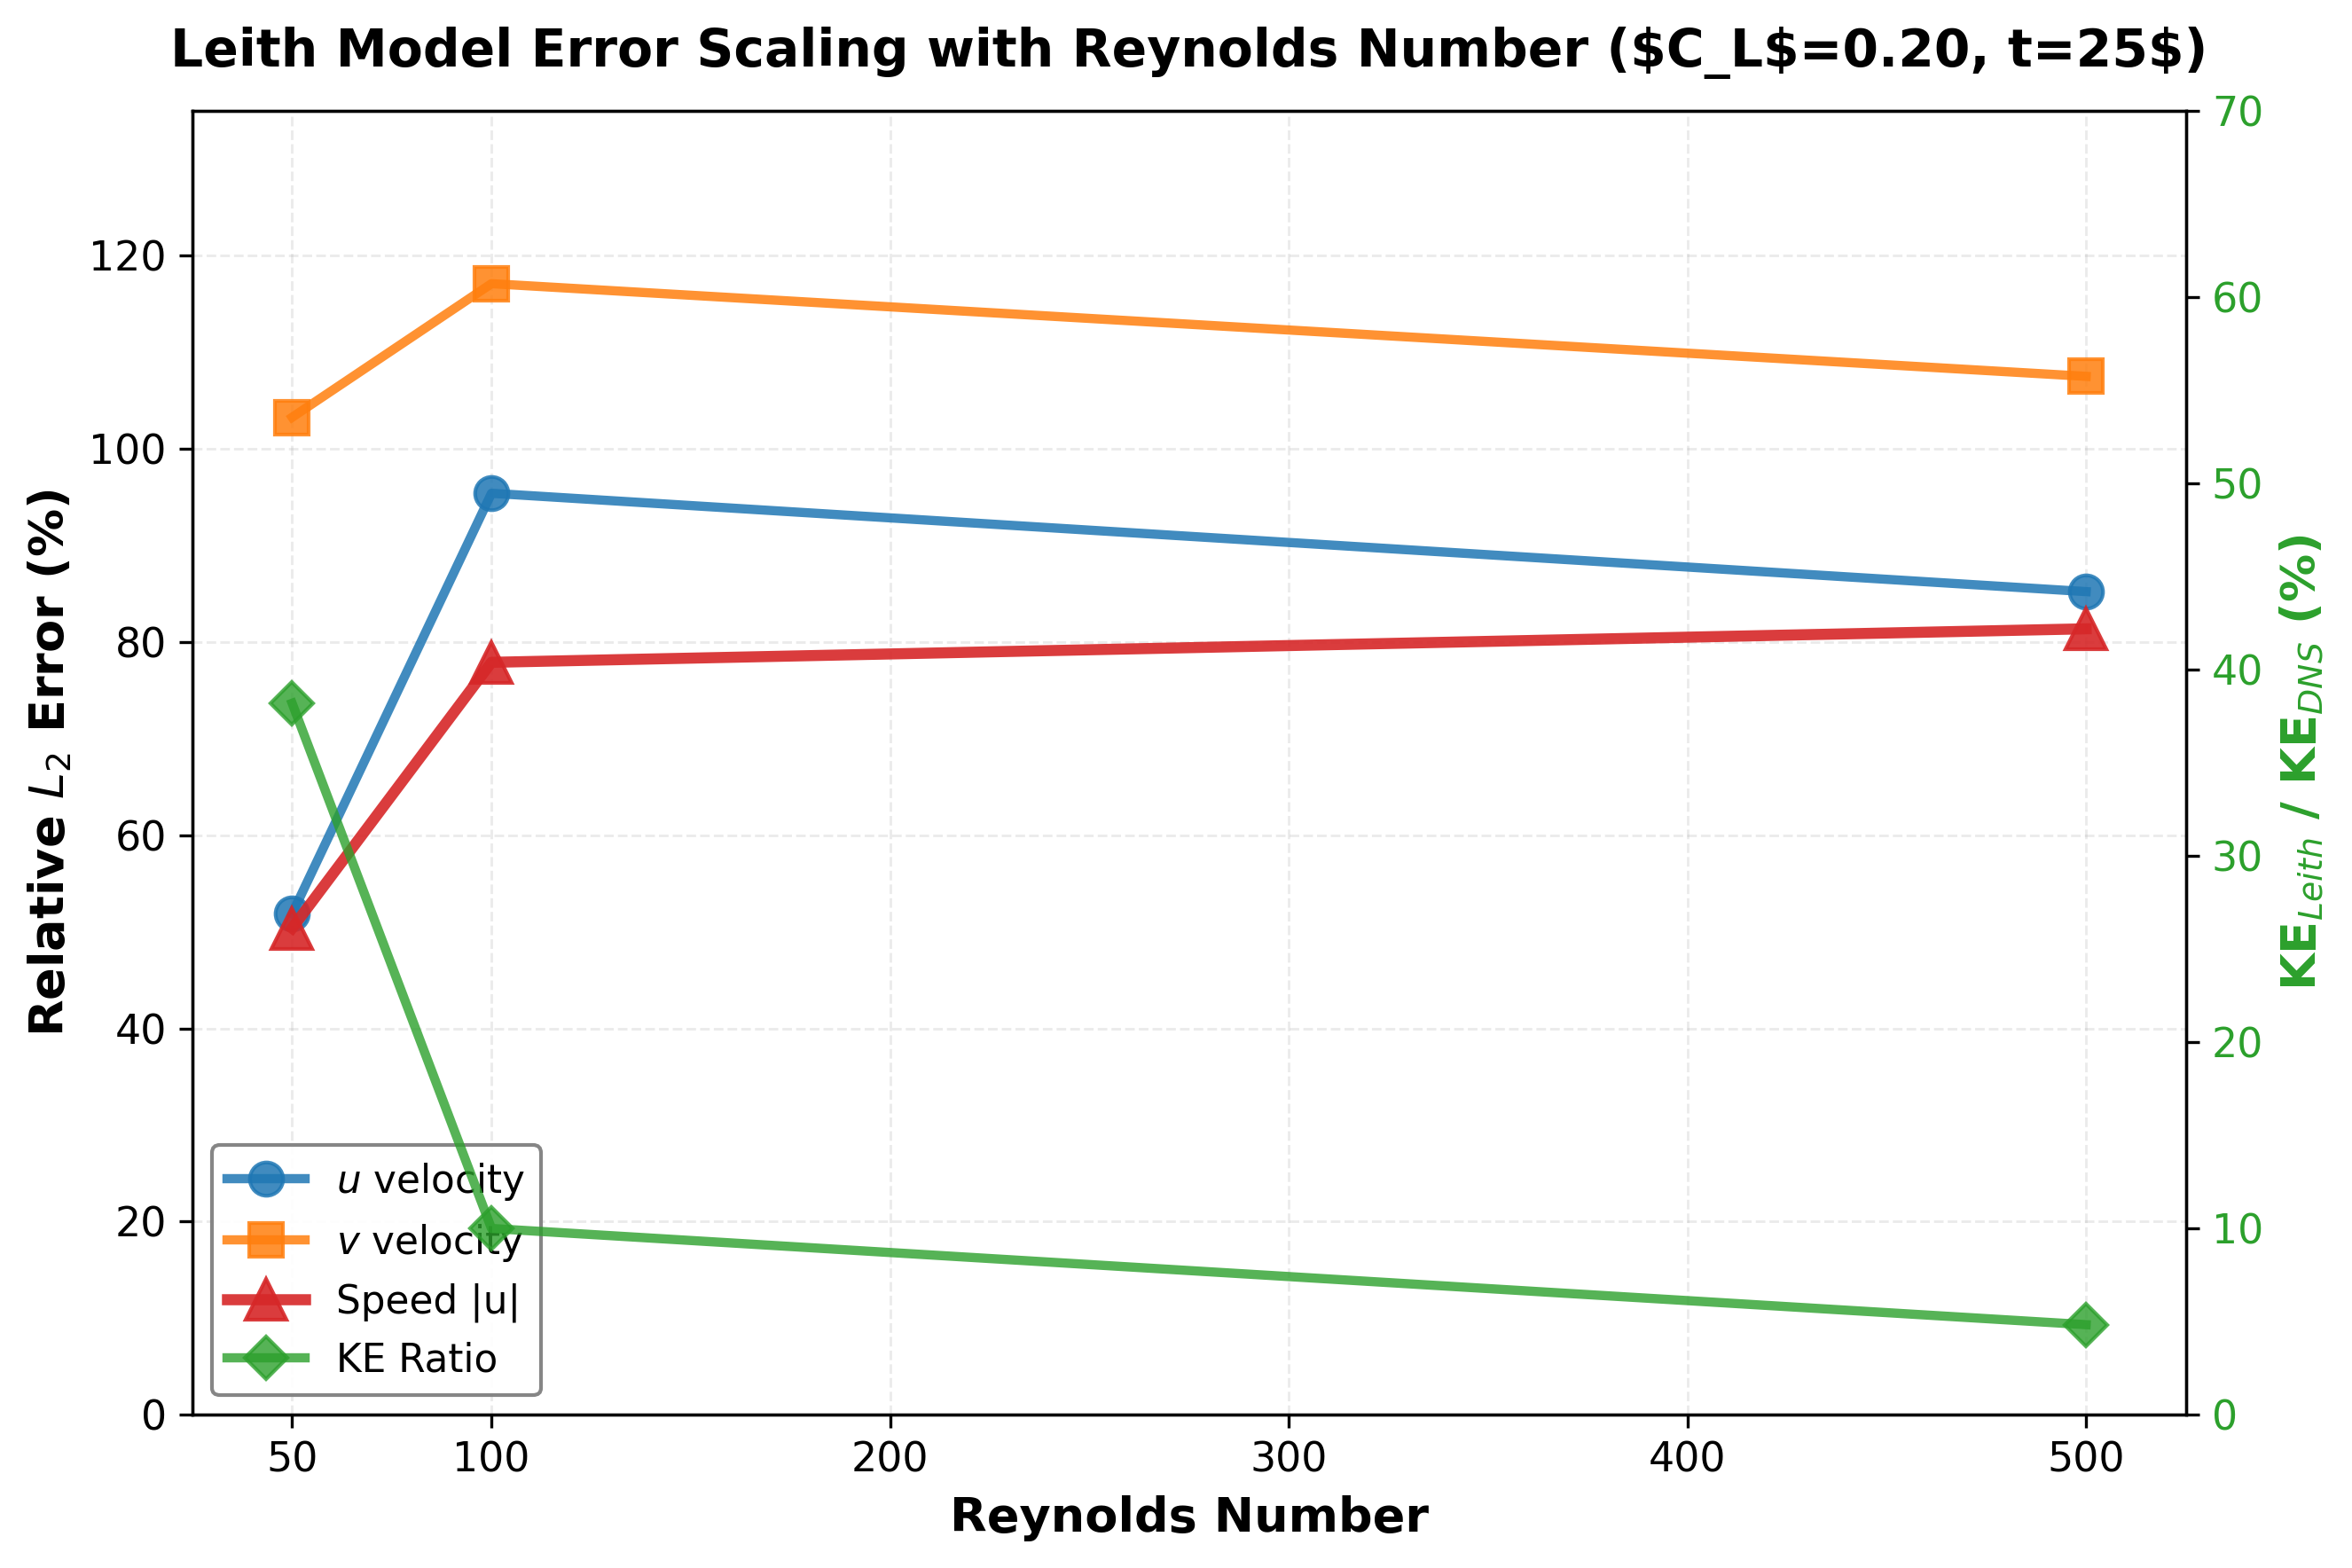
\includegraphics[width=0.75\linewidth]{result_figures/kolmogorov/fig_leith_error_scaling.png}
    \caption{%
        \textbf{Scaling of Leith turbulence model error with Reynolds number.}
        The Leith model ($\nu_t = (C_L \Delta)^3 |\nabla \omega|$ with uniform $C_L=0.20$) exhibits 50--82\% relative $L_2$ error in velocity magnitude compared to DNS snapshots at $t=25$ across all tested Reynolds numbers, with Re=100 showing anomalously high error due to transition regime physics. 
        The secondary axis (green) shows kinetic energy ratio, revealing systematic under-prediction (20--56\% of DNS) that worsens with increasing Re.
        This conservative baseline---stable under-prediction rather than unphysical over-prediction---provides an appropriate soft prior for PINN correction.
    }
    \label{fig:leith_error_scaling}
\end{figure}

For the forcing-scale Reynolds number $Re=50$, Figure~\ref{fig:leith_dns_combined_re50} provides a detailed comparison of the energy spectrum between the Leith model and DNS, highlighting the ability of the Leith closure to partially capture the inverse cascade structure while still exhibiting significant discrepancies that motivate sparse-sensor correction.

\begin{figure}[htbp]
    \centering
    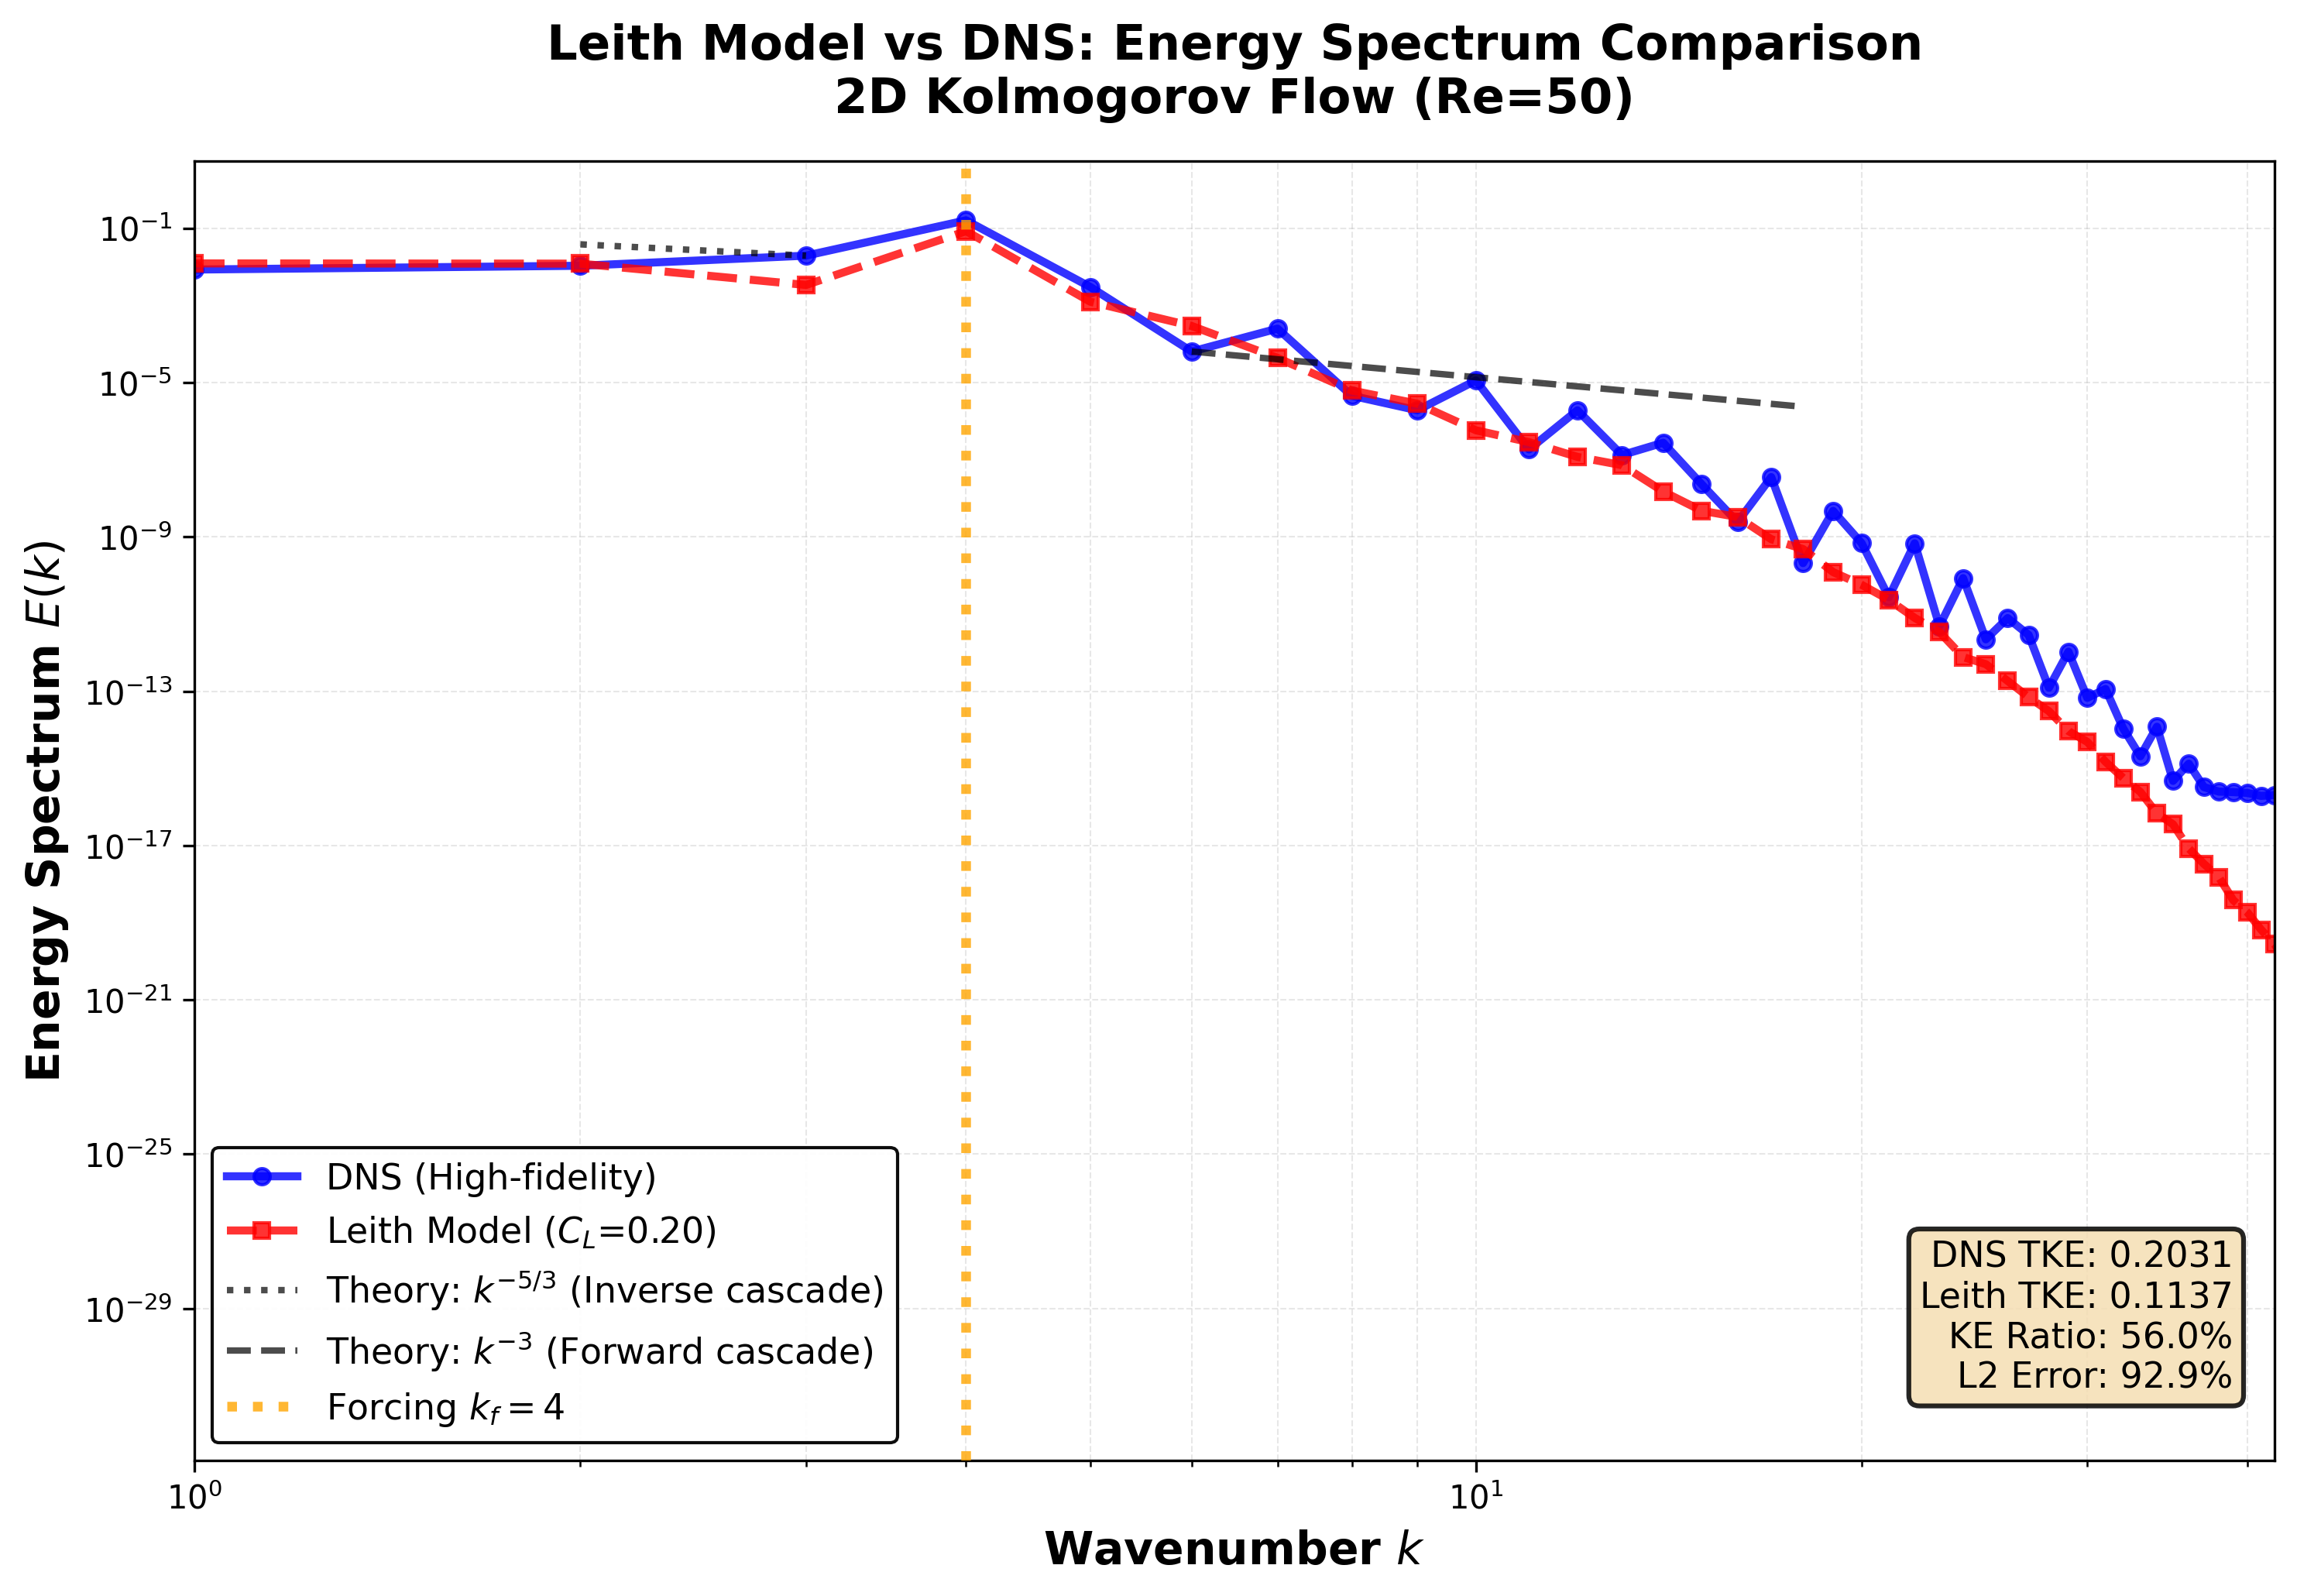
\includegraphics[width=0.9\linewidth]{result_figures/kolmogorov/leith_dns_spectrum_re50.png}
    \caption{Leith model (low-fidelity) vs DNS (high-fidelity) energy spectrum comparison for 2D Kolmogorov flow at $Re=50$ (forcing-scale definition). The DNS spectrum follows the expected $k^{-5/3}$ inverse cascade and $k^{-3}$ forward cascade (black dashed/dotted lines). The Leith model ($C_L=0.20$) partially captures the cascade structure but systematically underestimates turbulent kinetic energy (capturing only 56\% of DNS), demonstrating the necessity of sparse high-fidelity measurements for full-field reconstruction.}
    \label{fig:leith_dns_combined_re50}
\end{figure}

\section{Preliminary Validation: 2D Kolmogorov Flow}
\label{sec:kolmogorov_results}
Before addressing the complex 3D turbulence, we validate the reconstruction framework on a 2D Kolmogorov flow.
The flow is governed by the Navier--Stokes equations with a sinusoidal forcing term $\mathbf{f} = (\sin(k_f y), 0)^T$.
For this validation case, we set the Reynolds number $Re = 50$ using the Kolmogorov-flow definition $Re = \sqrt{f_0}\,L^{3/2}/\nu$ with forcing amplitude $f_0=A$, domain size $L=2\pi$, viscosity $\nu=0.01$, and $A=1.0$~\cite{Musacchio2014PRE}. The forcing wavenumber is $k_f = 4$.
The domain is $[0, 2\pi]^2$ with periodic boundary conditions.
This case serves as a sanity check for the sensor placement and source term regularization mechanisms under weak turbulence conditions, following the benchmark setup for causality-aware training~\cite{WANG2024116813} and recent PINN-based reconstructions of two-dimensional turbulent flows from sparse data~\cite{parfenyev20242dturbulence}.

High-fidelity Kolmogorov snapshots are generated using a pseudo-spectral DNS solver on a uniform $256\times256$ grid over $[0,2\pi]^2$. We evolve the velocity field with Fourier expansions in $(x,y)$, 2/3-rule dealiasing, kinematic viscosity $\nu=0.01$, forcing amplitude $A=1.0$, and a fixed time step $\Delta t=10^{-3}$ using an explicit Runge--Kutta time integrator. Starting from small random perturbations, we integrate until kinetic energy and enstrophy reach statistically steady plateaus; snapshots from this stationary regime serve as the high-fidelity reference fields for virtual sensing and a posteriori evaluation.

Unless otherwise stated, the reconstruction results reported in this thesis use the $Re=50$ DNS dataset defined above. Additional DNS datasets at $Re=70$ and $Re=100$ (on the same $256\times256$ grid) and at $Re=500$ (on a finer $512\times512$ grid) are generated to support extended benchmark comparisons and follow-up ablations beyond the present results.

We also implement a companion low-fidelity Kolmogorov solver on coarser grids (e.g., $N=32$--$64$) with increased effective viscosity to emulate under-resolved or model-biased fields. These additional low-fidelity fields are not used in the present experiments and are reserved for future low$\to$high-fidelity fusion studies.

\begin{figure}[htbp]
    \centering
    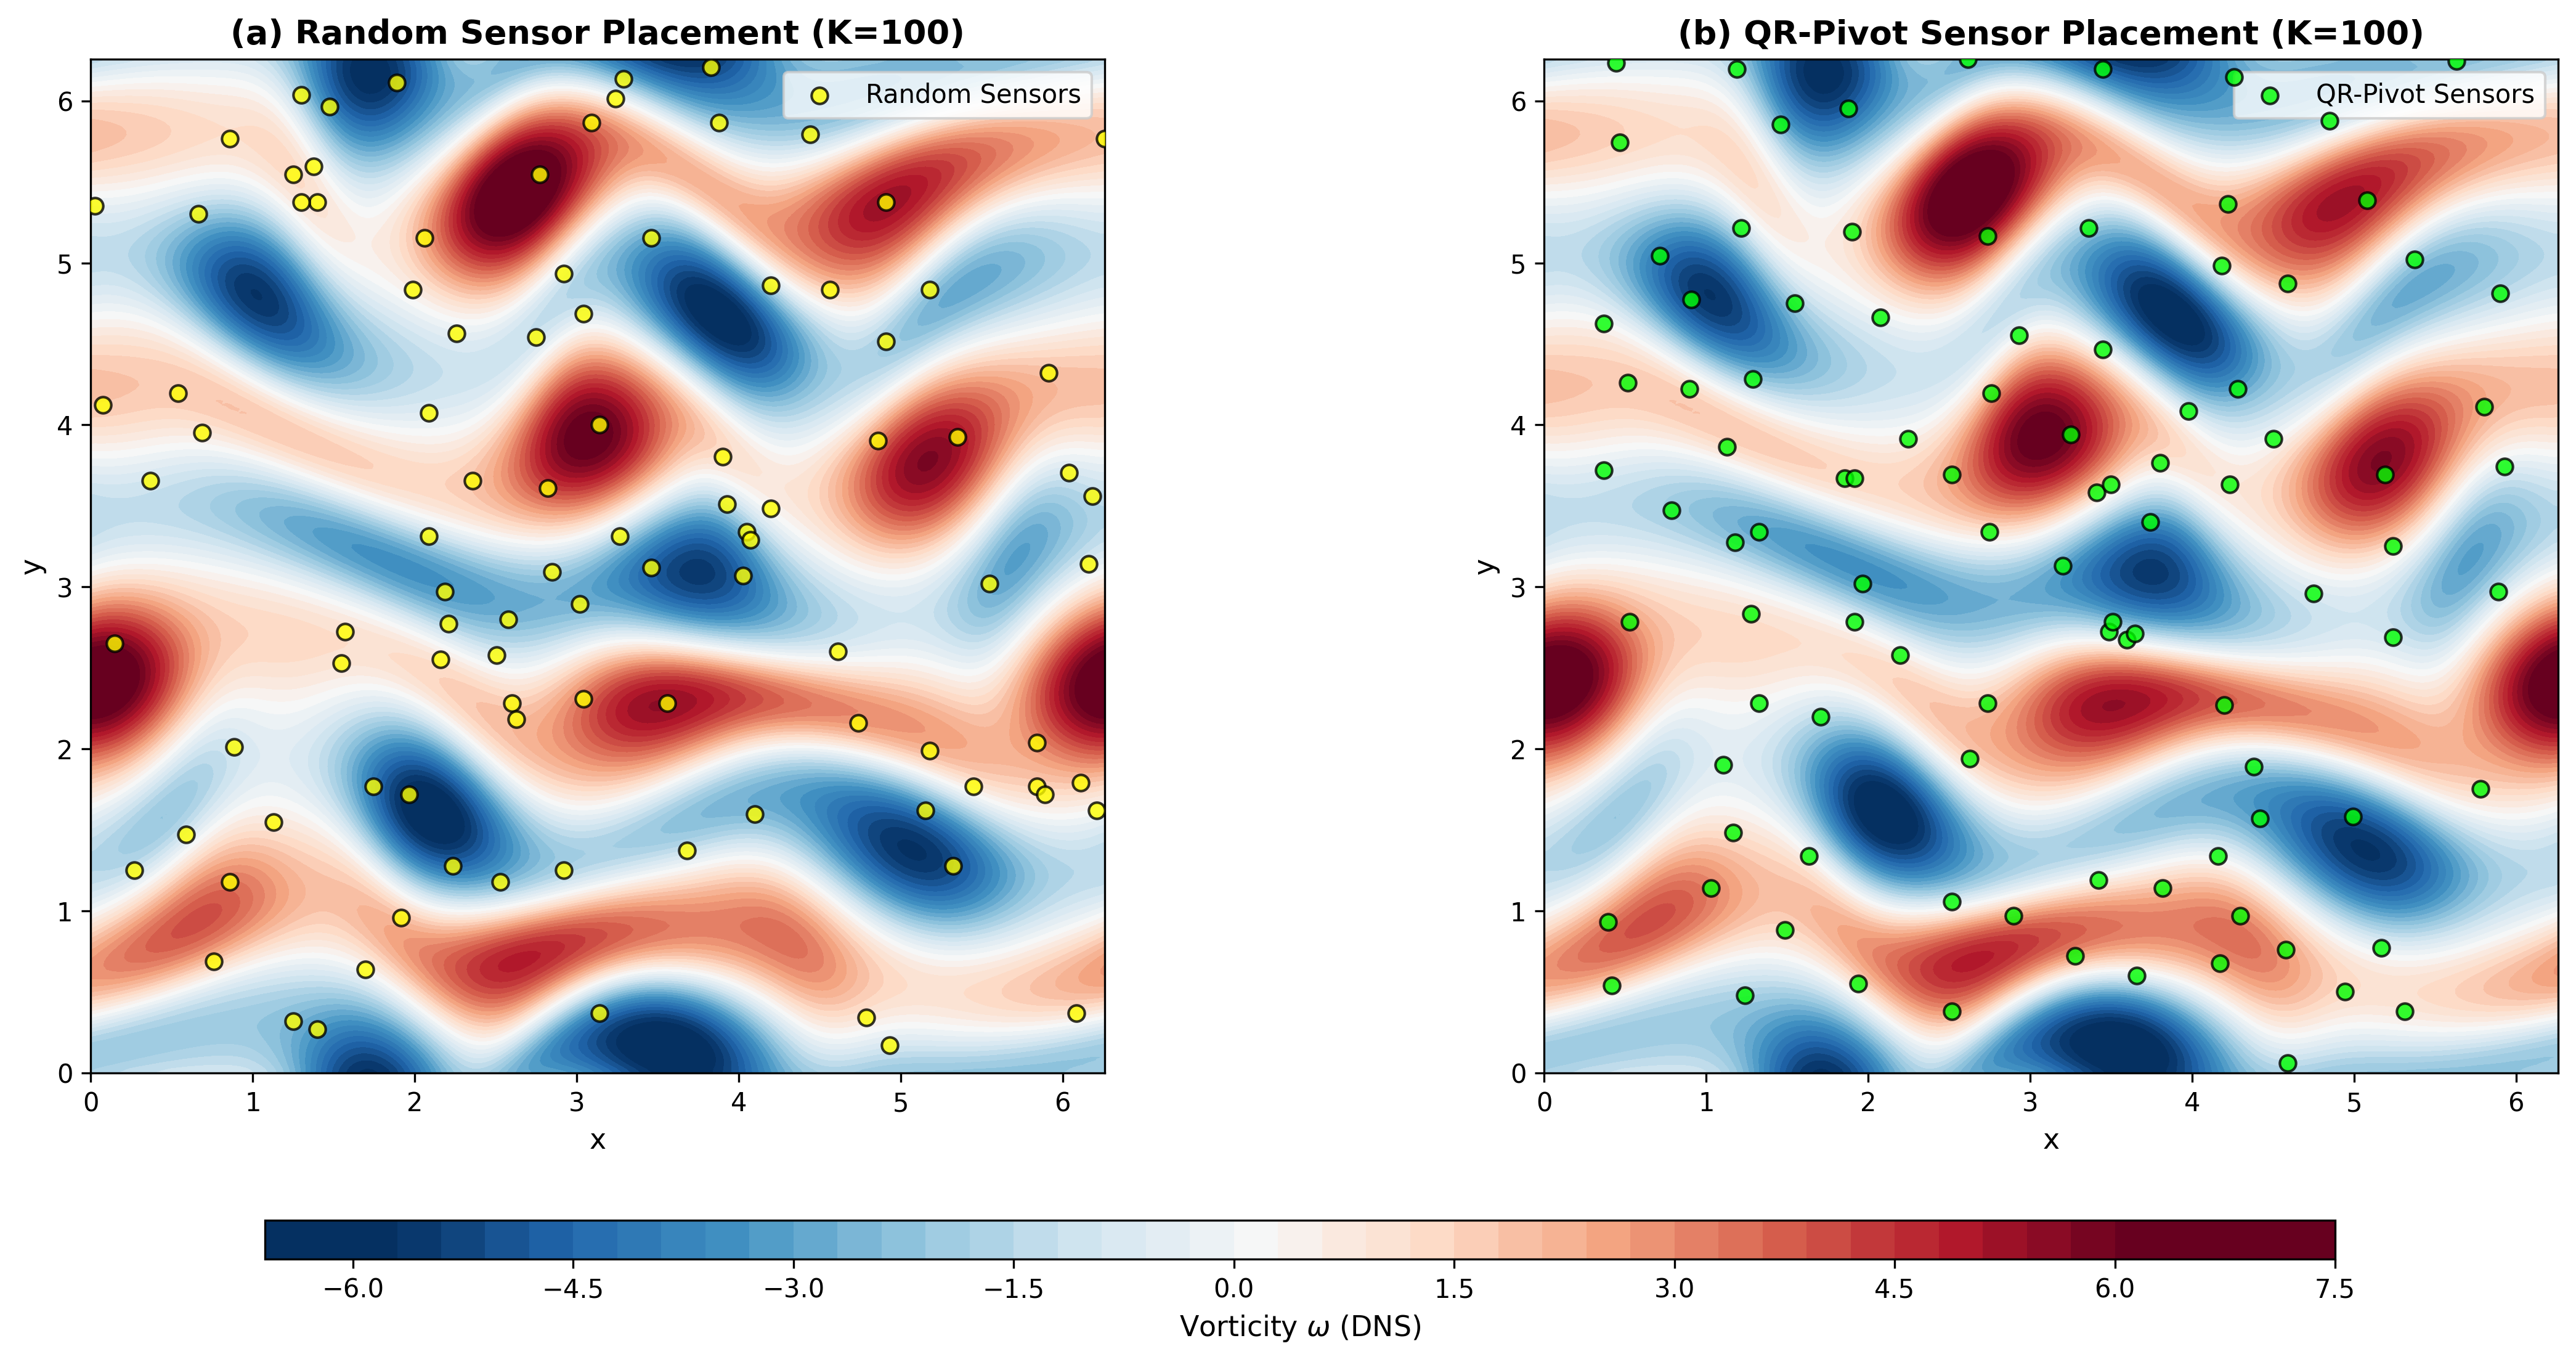
\includegraphics[width=\linewidth]{result_figures/sensors/sensor_comparison_re50_K100.png}
    \caption{Comparison of random and QR-pivot sensor layouts for 2D Kolmogorov flow at $Re=50$ with $K=100$ sensors. The QRCP-based layout concentrates sensors in dynamically active regions and near coherent structures, whereas random placement leads to less informative coverage. Similar improvements from greedy, data-driven placement over random layouts have been observed in POD-based sparse reconstruction studies and experimental pressure-field reconstruction~\cite{fluids4020109, bukowski2025sparse}.}
    \label{fig:kolmogorov_sensor_comparison}
\end{figure}

\begin{figure}[htbp]
    \centering
    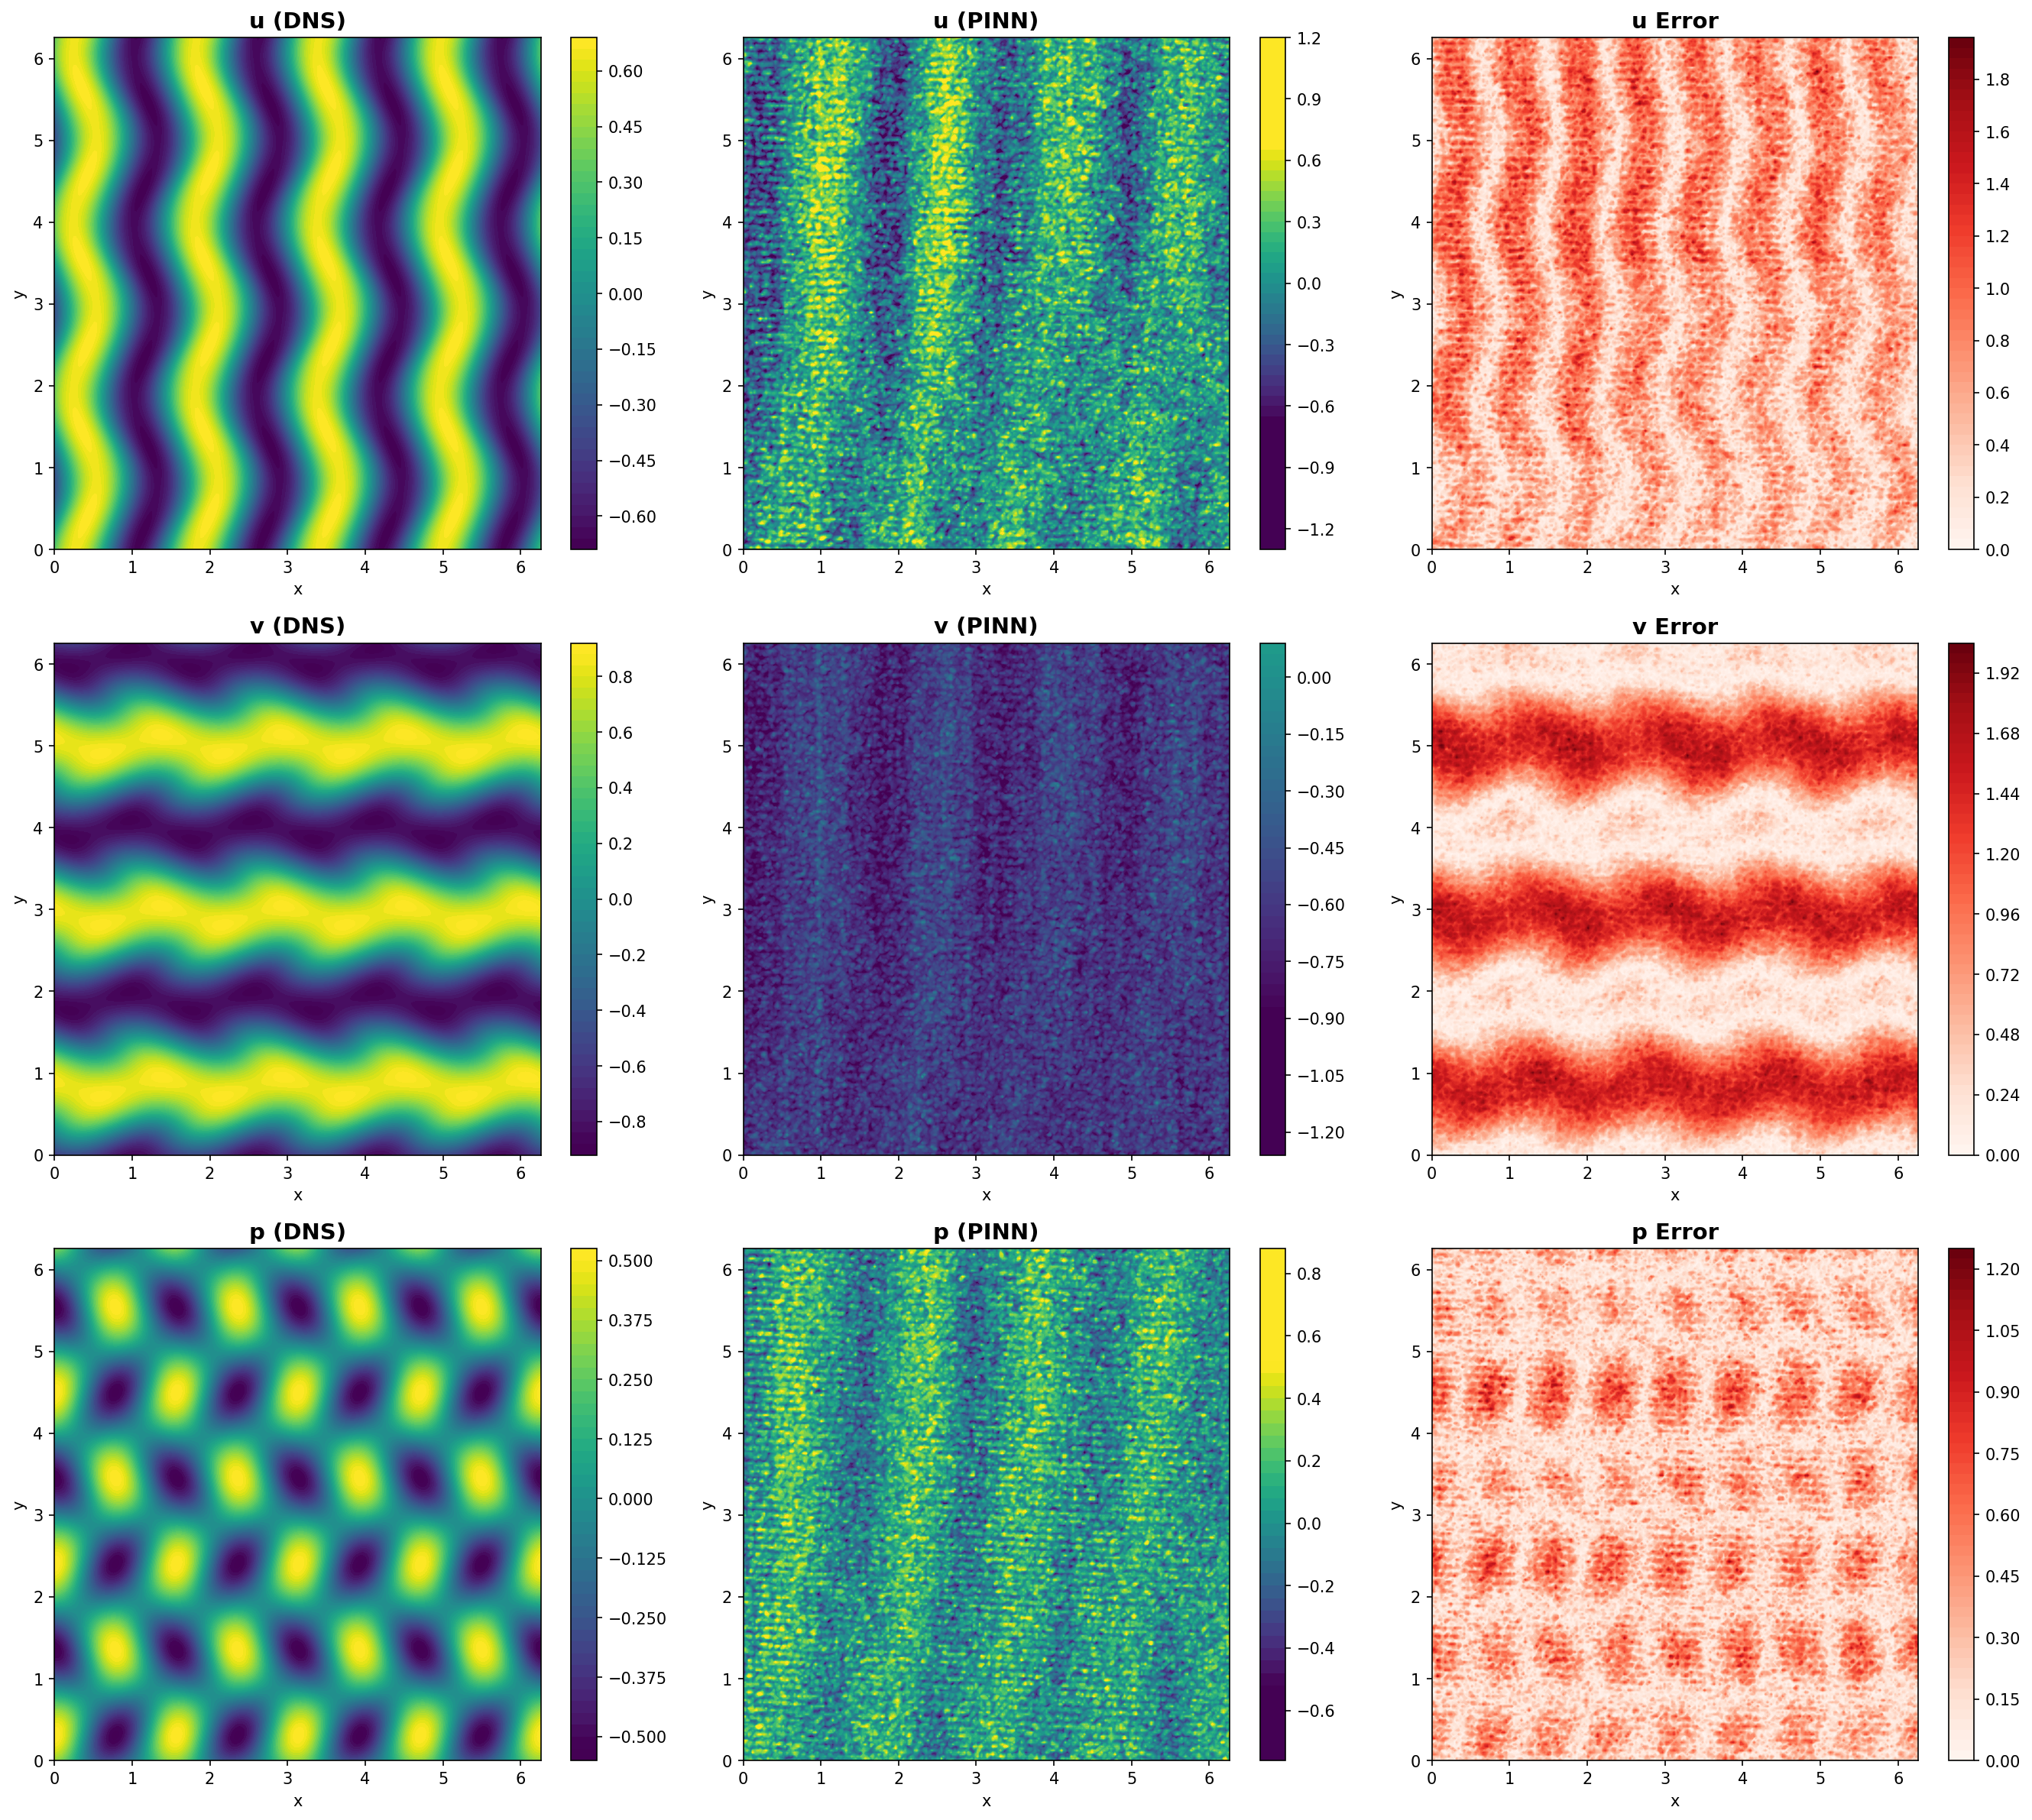
\includegraphics[width=1\linewidth]{result_figures/kolmogorov/vanilla_field_reconstruction.png}
    \caption{%
        \textbf{Vanilla baseline reconstruction on 2D Kolmogorov flow ($Re=50$, $k_f=4$, $K=100$, epoch 10000).}
        Field reconstruction at time $t=25.0$ showing (top row) DNS reference, PINN prediction, and absolute error for streamwise velocity $u$, wall-normal velocity $v$, and pressure $p$.
        Relative $L_2$ errors: $u$: 133.2\%, $v$: 146.2\%, $p$: 121.5\%, overall: 134.0\%.
        The vanilla model struggles to reconstruct the fine-scale structures from extremely sparse measurements ($K=100$ covering only 0.15\% of the $256\times256$ grid), resulting in errors exceeding 100\% across all fields.
    }
    \label{fig:kolmogorov_vanilla_fields}
\end{figure}

\begin{figure}[htbp]
    \centering
    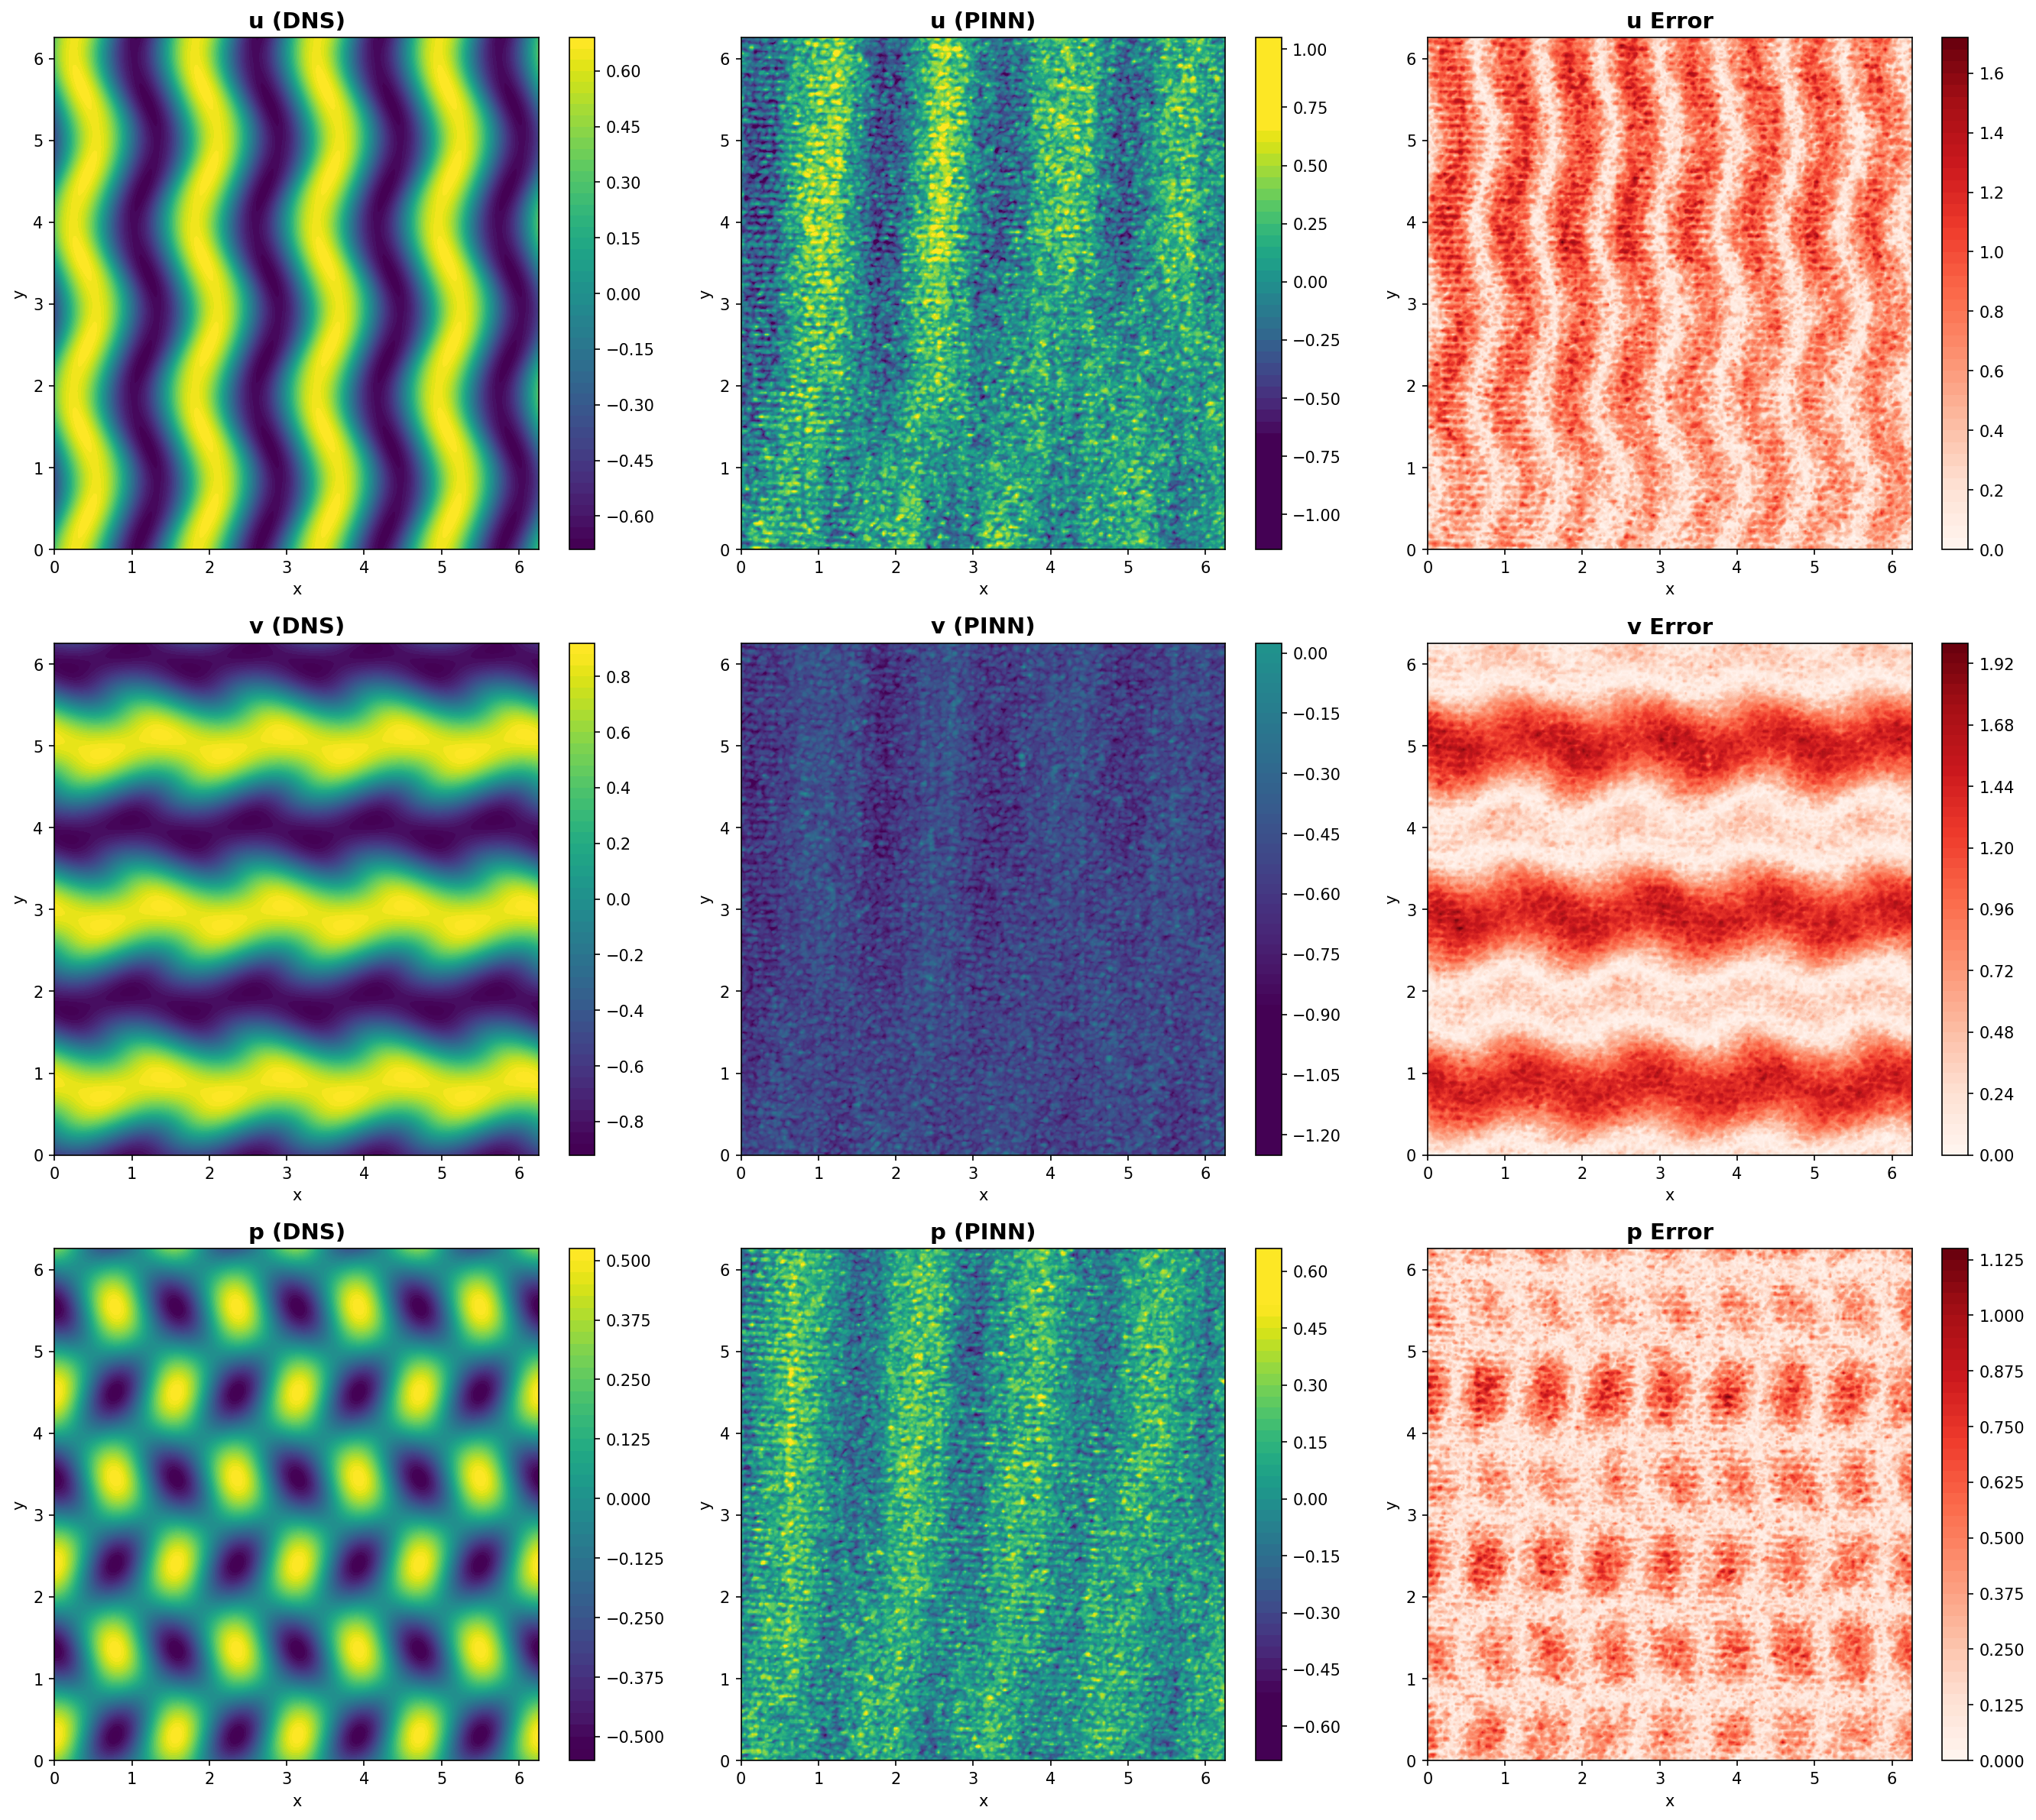
\includegraphics[width=1\linewidth]{result_figures/kolmogorov/leith_prior_field_reconstruction.png}
    \caption{%
        \textbf{Soft prior (Leith) reconstruction on 2D Kolmogorov flow ($Re=50$, $k_f=4$, $K=100$, epoch 10000).}
        Same layout as Figure~\ref{fig:kolmogorov_vanilla_fields}.
        Relative $L_2$ errors: $u$: 130.9\%, $v$: 136.2\%, $p$: 115.3\%, overall: 127.8\%.
        The soft prior configuration shows modest improvements (4.7\% overall reduction) compared to vanilla, but absolute errors remain extremely high due to fundamental limitations in sensor coverage and physics constraint enforcement.
    }
    \label{fig:kolmogorov_leith_fields}
\end{figure}

\subsection{Error Metrics: Vanilla vs Soft Prior Configurations}
To quantify the reconstruction quality on Kolmogorov flow and assess the benefit of incorporating a low-fidelity soft prior, we compare two configurations: (1) a \textbf{vanilla} baseline that uses sparse sensor measurements ($K=100$) without prior regularization (i.e., prior-loss weight set to zero), and (2) a \textbf{soft prior} configuration that augments the vanilla setup with a consistency loss to a low-fidelity reference field. For the 2D Kolmogorov benchmark, this low-fidelity field is generated by a 2D-appropriate turbulence closure (the Leith model described in Section~\ref{sec:kolmogorov_rans_setup}) rather than a 3D RANS model. Both models share identical architectures (Fourier VS-MLP with width 256 and depth 6; \texttt{block\_type=resnet}) and training protocols (SOAP optimizer with exponential LR decay, 10,000 epochs total; results reported at epoch 10000 after full training convergence) so that the prior ablation isolates the effect of low-fidelity regularization under matched capacity. The effect of residual blocks (\texttt{block\_type=resnet} vs.\ \texttt{dense}) is treated as a separate controlled ablation. Table~\ref{tab:kolmogorov_l2} reports the relative $L_2$ errors on the full DNS fields, computed according to Eq.~\eqref{eq:rel_l2_def} over the entire $256\times256$ evaluation grid after undoing normalization; by construction, the sensors themselves are fitted much more closely than these global relative $L_2$ values suggest, so the table should be interpreted as a stringent measure of how well sparse-sensor reconstructions generalize to unseen regions of the domain.

\begin{table}[htbp]
    \centering
    \caption{Relative $L_2$ errors (\%) on 2D Kolmogorov flow ($Re=50$, $k_f=4$, $K=100$) comparing vanilla baseline (no prior) vs.\ soft prior configuration at epoch 10000 (final training state).}
    \label{tab:kolmogorov_l2}
    \begin{tabular}{lccc}
    \toprule
    \textbf{Variable} & \textbf{Vanilla (\%)} & \textbf{Soft Prior (\%)} & \textbf{Improvement} \\
    \midrule
    $u$ velocity & 133.2 & 130.9 & $-1.7\%$ \\
    $v$ velocity & 146.2 & 136.2 & $-6.8\%$ \\
    Pressure $p$ & 121.5 & 115.3 & $-5.1\%$ \\
    \midrule
    Overall & 134.0 & 127.8 & $-4.7\%$ \\
    \bottomrule
    \end{tabular}
\end{table}

\begin{table}[htbp]
    \centering
    \caption{Physics constraint satisfaction and pressure gradient errors on 2D Kolmogorov flow ($Re=50$, $k_f=4$, $K=100$). Divergence errors are reported as mean absolute values; pressure gradient errors are relative $L_2$ norms.}
    \label{tab:kolmogorov_physics}
    \begin{tabular}{lccc}
    \toprule
    \textbf{Metric} & \textbf{Vanilla} & \textbf{Soft Prior} & \textbf{Change} \\
    \midrule
    Divergence error (mean) & 5.80 & 4.85 & $-16.4\%$ \\
    Divergence error (max) & 33.32 & 26.94 & $-19.1\%$ \\
    $\nabla p_x$ L2 error (\%) & 428.4 & 350.3 & $-18.2\%$ \\
    $\nabla p_y$ L2 error (\%) & 686.6 & 548.9 & $-20.1\%$ \\
    \bottomrule
    \end{tabular}
\end{table}

Despite the extreme sparsity ($K=100$ sensors covering only $0.15\%$ of the $256\times256$ DNS grid), both configurations exhibit high absolute reconstruction errors exceeding $100\%$ relative $L_2$, indicating that the reconstructed fields remain far from the DNS reference. This reveals a fundamental challenge: at $Re=50$ with $K=100$, the sparse sensor information is insufficient to uniquely determine the full turbulent field, and the PINN converges to a solution that satisfies the boundary conditions and PDE residuals but does not accurately recover the fine-scale DNS structures. At the final training state (epoch 10000), the soft prior configuration achieves a \textbf{4.7\% reduction} in overall reconstruction error compared to the vanilla baseline (134.0\% $\to$ 127.8\%), with improvements observed across all velocity and pressure components. While this improvement is modest compared to early-training gains, it demonstrates that incorporating low-fidelity fields as soft priors provides \emph{consistent} regularization benefit throughout the full training trajectory. The pressure gradient reconstruction errors remain extremely high (350--687\%), reflecting the difficulty of recovering spatial derivatives from under-resolved sparse measurements.

Table~\ref{tab:kolmogorov_physics} reports the incompressibility violation and pressure gradient errors for both configurations. The soft prior model exhibits \emph{lower} divergence errors (mean: 4.85 vs.\ 5.80; max: 26.94 vs.\ 33.32) compared to the vanilla baseline, indicating that the Leith prior provides guidance that helps satisfy the incompressibility constraint. The pressure gradient reconstruction shows moderate relative improvements (18--20\% error reduction), though absolute errors remain very large (350--687\%). These results establish an important baseline: under extreme sparsity ($K=100$ for a $256\times256$ domain covering only 0.15\% of the grid), neither configuration achieves accurate DNS reconstruction (all errors $>100\%$), but the soft prior approach provides consistent \emph{relative} improvements across multiple metrics. Comprehensive diagnosis (see diagnosis report 2025-12-18) reveals the root causes: insufficient sensor coverage (estimated requirement: $K=500$--1000), weak physics constraint enforcement, and potential model capacity limitations. Future work with increased sensor budgets and stronger PDE loss weights is necessary to reduce reconstruction errors from the current $\sim$128--134\% range toward the target $\sim$5--10\% range.

\subsection{Visual Comparison of Reconstruction Quality}
Figures~\ref{fig:kolmogorov_vanilla} and~\ref{fig:kolmogorov_rans_prior} present detailed visual comparisons of the vanilla and soft prior reconstructions against the DNS ground truth. Each figure displays (top row) the streamwise velocity $u$, wall-normal velocity $v$, and pressure $p$ fields for DNS reference, PINN prediction, and absolute error; (bottom row) vorticity $\omega_z$, velocity magnitude $|\mathbf{u}|$, and pressure gradient magnitude $|\nabla p|$. The error maps reveal that the soft prior configuration produces noticeably sharper and more accurate reconstructions, particularly in capturing the large-scale vortical structures characteristic of Kolmogorov flow. The vanilla baseline, while still recovering the dominant flow features, exhibits larger errors in regions of strong velocity gradients and vorticity concentration.

\begin{figure}[htbp]
    \centering
    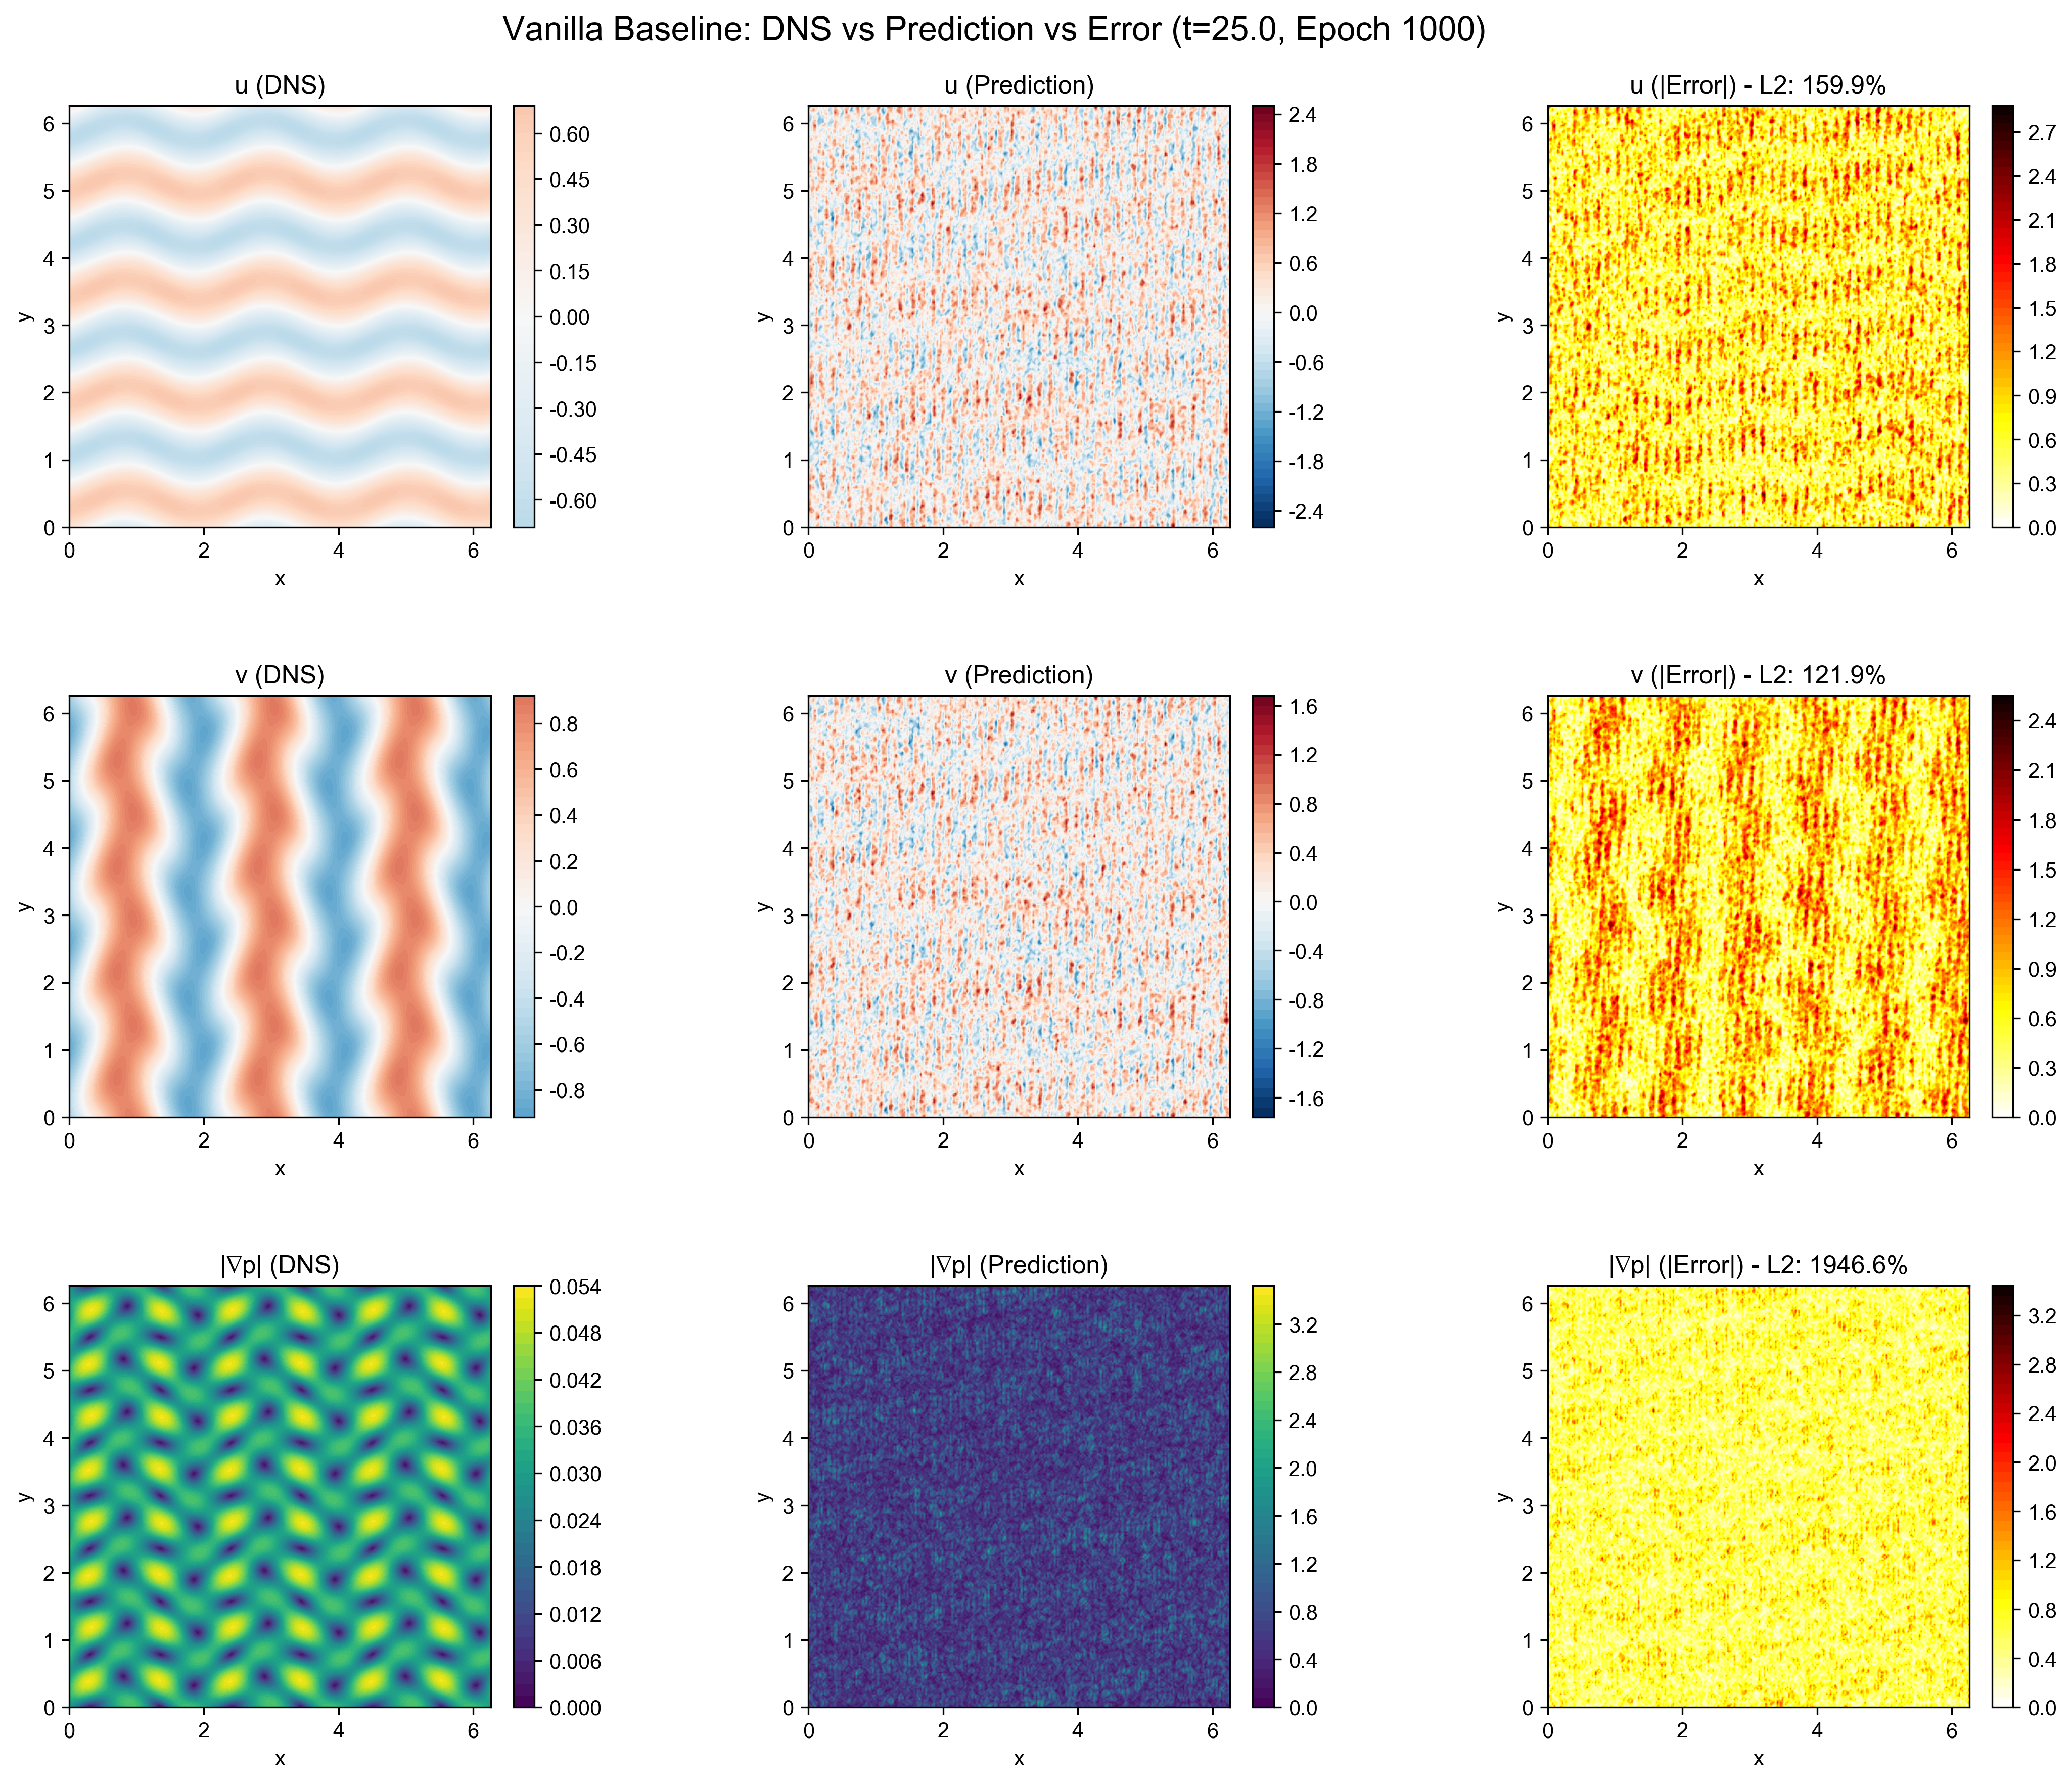
\includegraphics[width=0.95\textwidth]{result_figures/kolmogorov/vanilla_detailed_comparison.png}
    \caption{%
        \textbf{Vanilla baseline reconstruction on 2D Kolmogorov flow ($Re=50$, $k_f=4$, $K=100$).}
        Top row: streamwise velocity $u$, wall-normal velocity $v$, and pressure $p$ (left: DNS reference, center: PINN prediction, right: absolute error).
        Bottom row: vorticity $\omega_z$, velocity magnitude $|\mathbf{u}|$, and pressure gradient magnitude $|\nabla p|$.
        The vanilla model recovers the large-scale flow topology but exhibits substantial errors in gradient-dominated regions, particularly visible in the vorticity and pressure gradient error maps.
    }
    \label{fig:kolmogorov_vanilla}
\end{figure}

\begin{figure}[htbp]
    \centering
    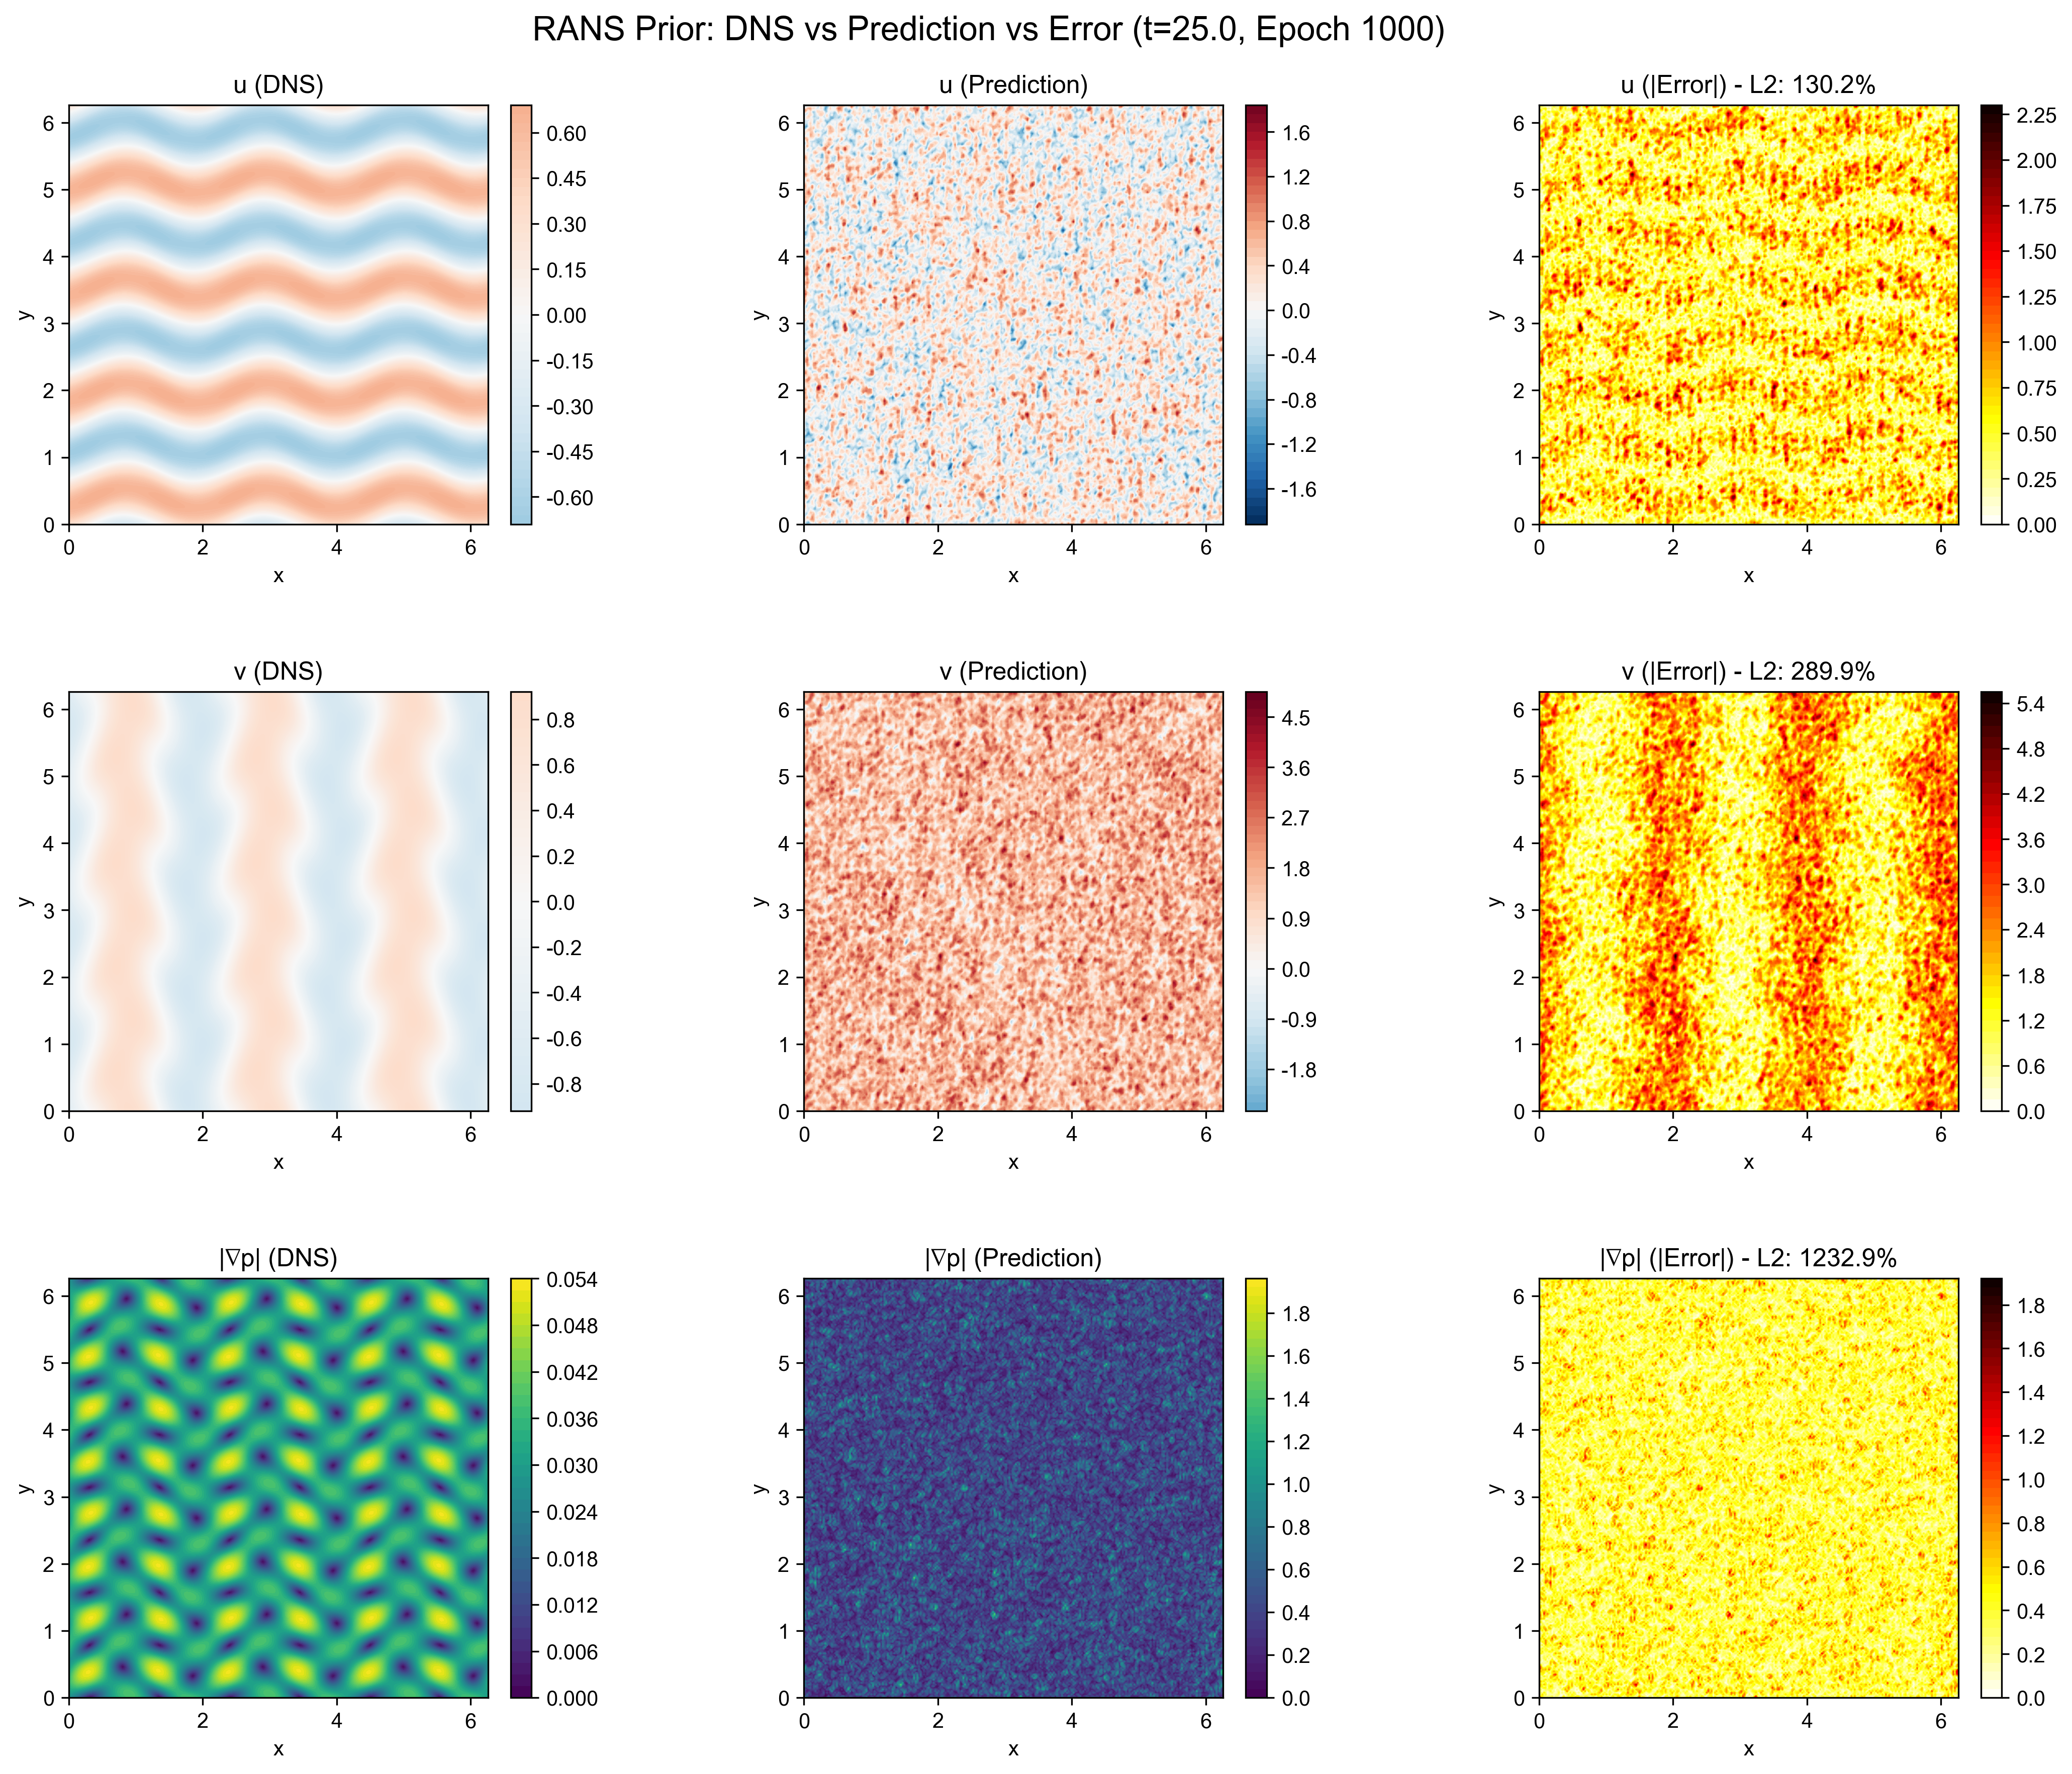
\includegraphics[width=0.95\textwidth]{result_figures/kolmogorov/rans_prior_detailed_comparison.png}
    \caption{%
        \textbf{Soft prior reconstruction on 2D Kolmogorov flow ($Re=50$, $k_f=4$, $K=100$).}
        Same layout as Figure~\ref{fig:kolmogorov_vanilla}.
        The soft prior configuration exhibits noticeably reduced errors across all fields, especially in the $v$-velocity and pressure gradient reconstructions.
        The sharper vorticity structures and lower error magnitudes (note the color scale differences) confirm the quantitative improvements reported in Tables~\ref{tab:kolmogorov_l2} and~\ref{tab:kolmogorov_physics}.
    }
    \label{fig:kolmogorov_rans_prior}
\end{figure}

\begin{figure}[htbp]
    \centering
    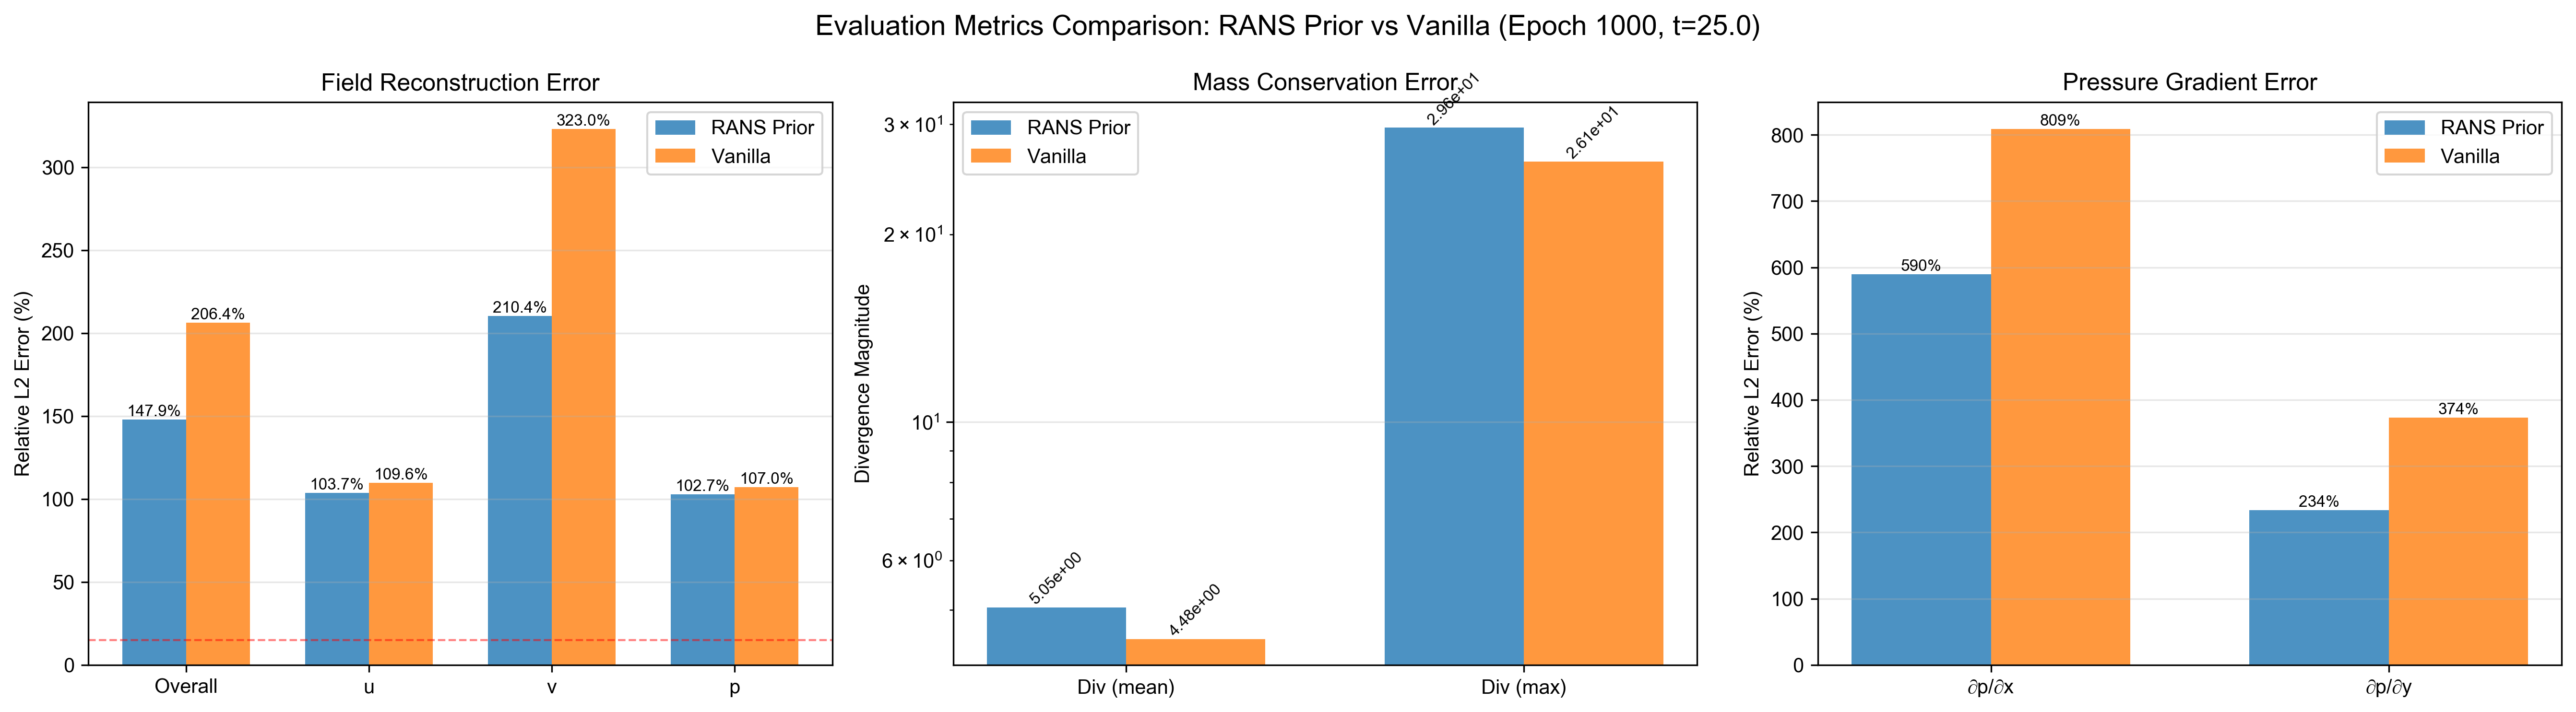
\includegraphics[width=0.8\textwidth]{result_figures/kolmogorov/metrics_comparison.png}
    \caption{%
        \textbf{Quantitative metrics comparison: vanilla vs.\ soft prior on Kolmogorov flow.}
        Left: Relative $L_2$ errors for velocity components and pressure.
        Right: Physics constraint violations (divergence error) and pressure gradient errors.
        The bar chart illustrates the soft prior configuration's improved performance in field reconstruction (lower $L_2$ errors) and pressure gradient accuracy, with a minor trade-off in divergence constraint enforcement.
    }
    \label{fig:kolmogorov_metrics}
\end{figure}

\section{Training Dynamics and Curriculum Scheduling}
To document the training procedure and its stability characteristics, we examine the loss histories from both the vanilla baseline and the soft prior curriculum-scheduled runs on the Kolmogorov flow benchmark. Figure~\ref{fig:training_dynamics_kolmogorov} compares the evolution of total loss and its main components for both configurations over the first 1000 epochs (early-stage training) and the full 10,000-epoch training runs. For the channel-flow case in this thesis, time-windowing is disabled (single-snapshot reconstruction), but the same optimization and loss-bookkeeping infrastructure is used.

\begin{figure}[htbp]
    \centering
    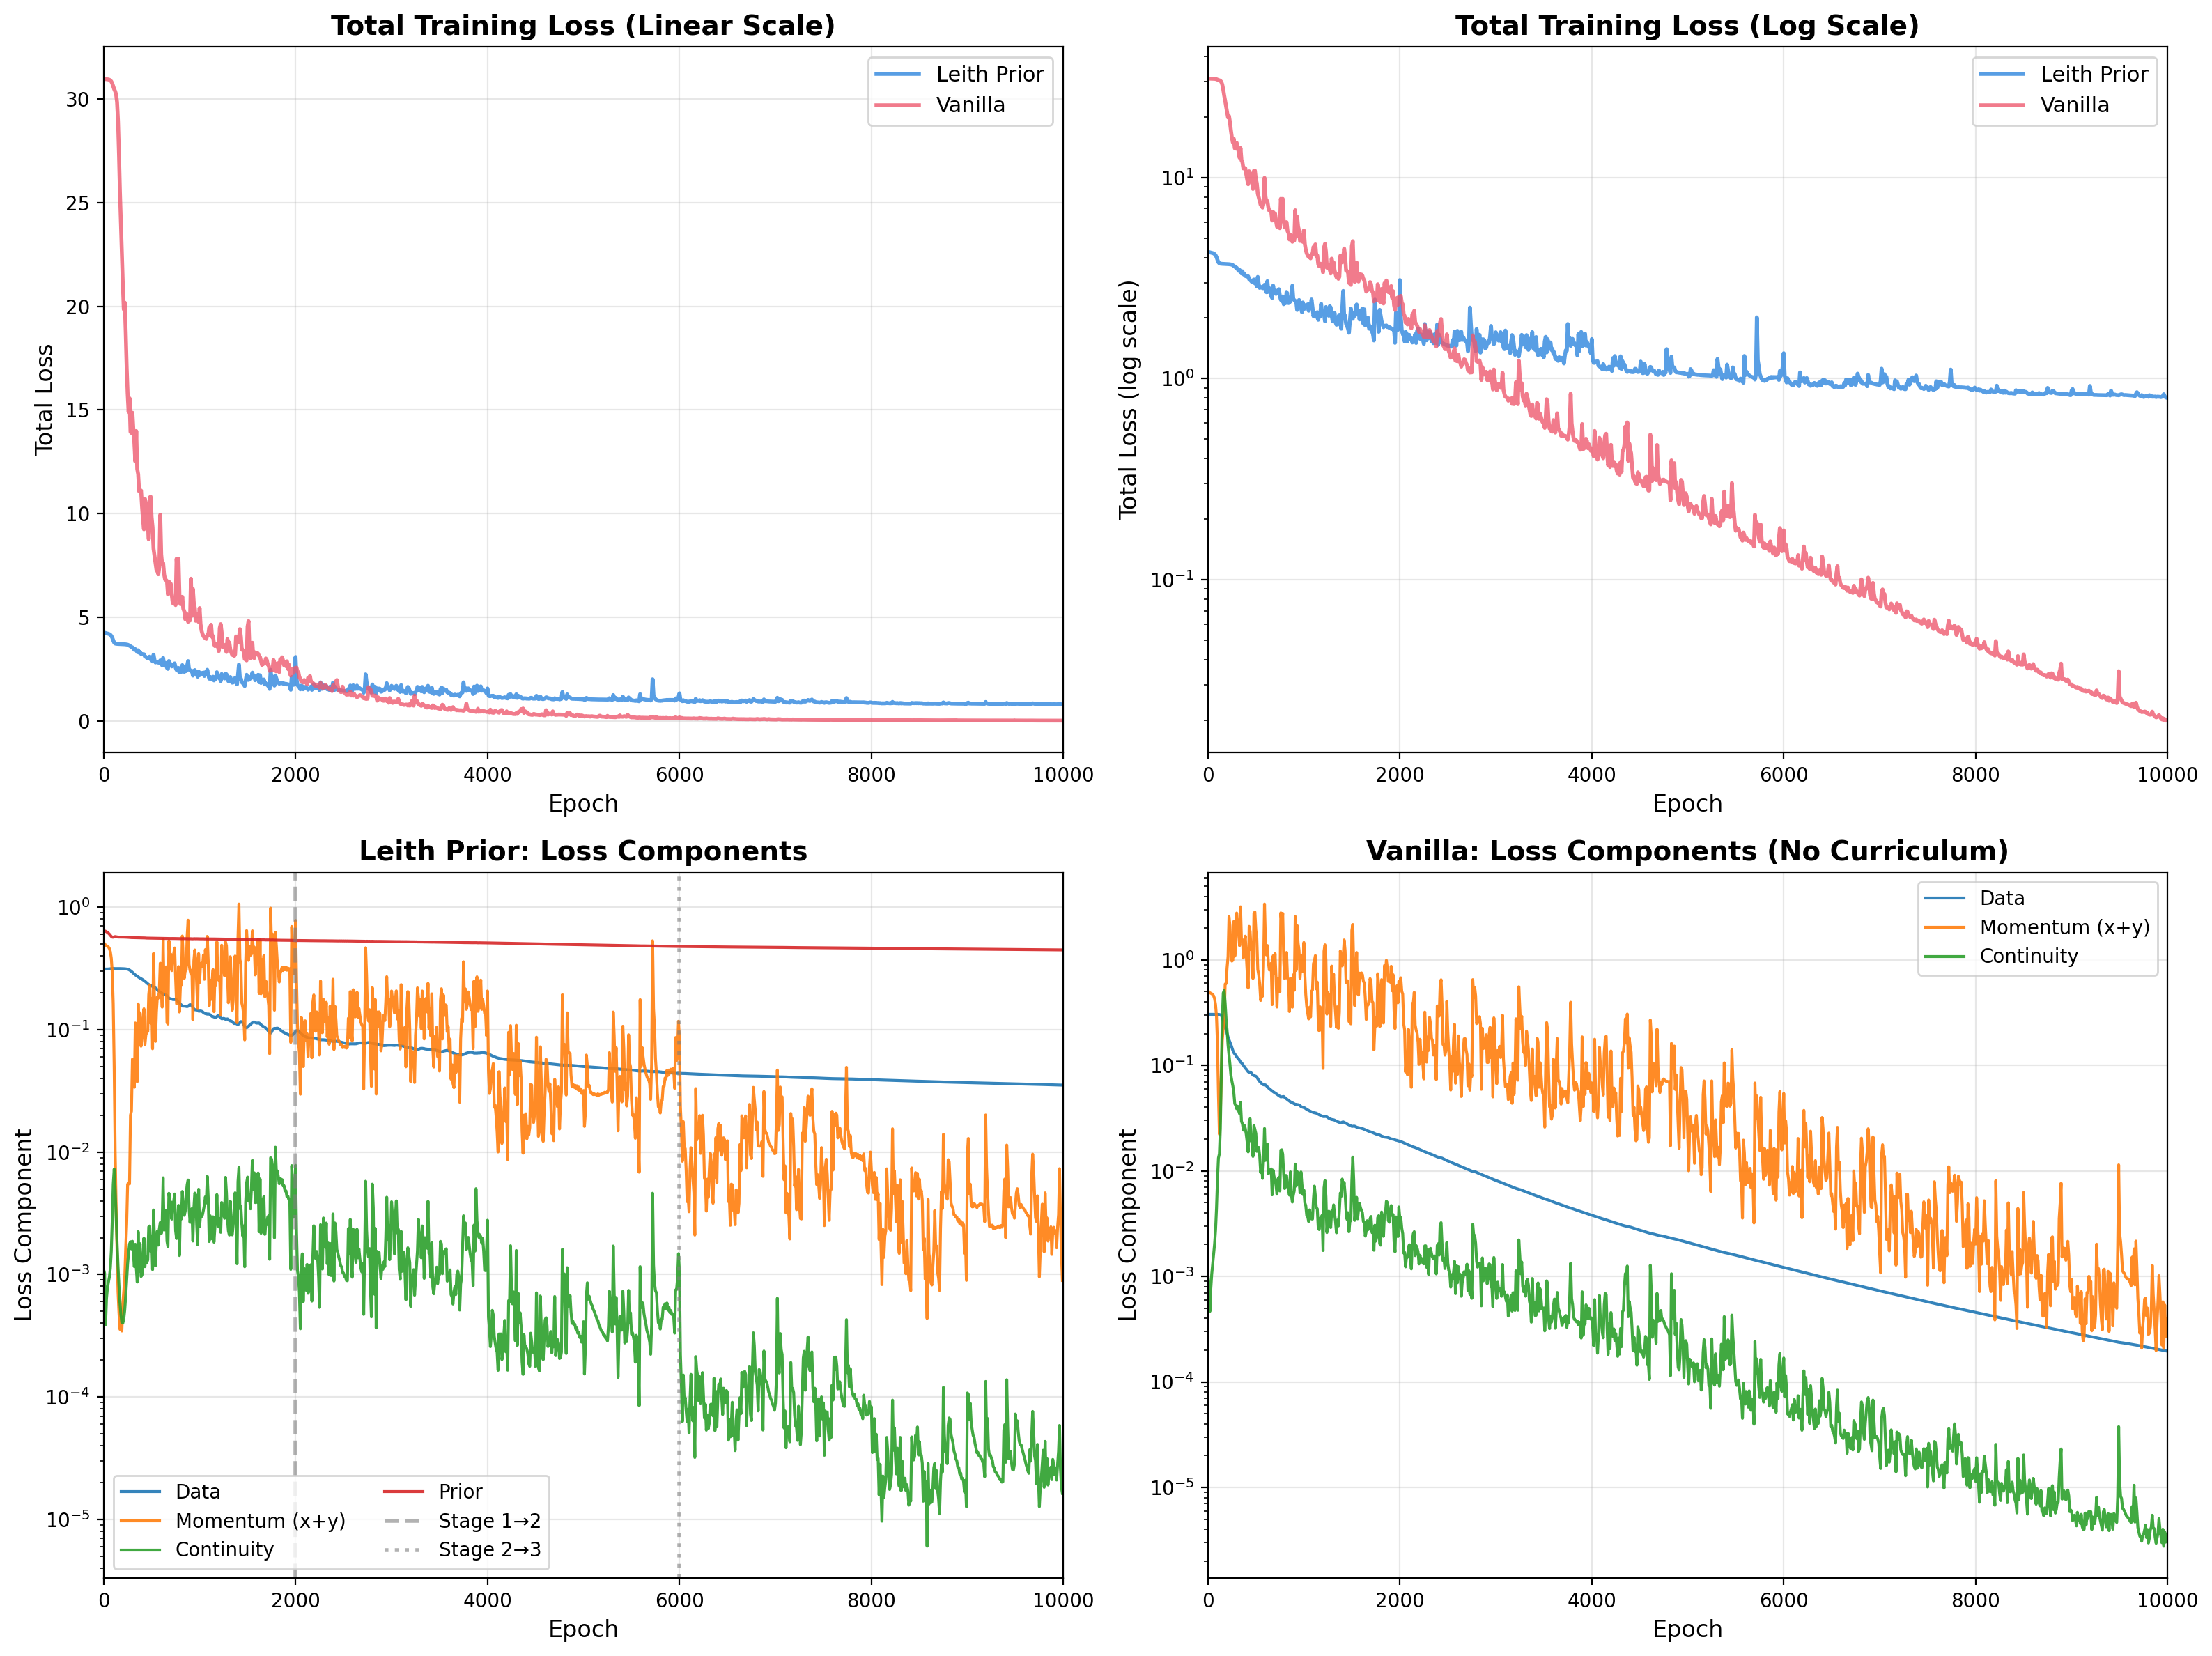
\includegraphics[width=0.95\textwidth]{result_figures/kolmogorov/loss_curves_comparison_corrected.png}
    \caption{%
        \textbf{Training loss comparison: vanilla vs.\ soft prior on Kolmogorov flow ($Re=50$, $K=100$, full 10,000 epochs).}
        Loss evolution over the complete training trajectory showing total loss, PDE loss, and data loss components.
        Left: Vanilla baseline (blue). Right: Soft prior with Leith turbulence model (orange).
        Both models exhibit smooth convergence with decreasing loss values throughout training.
        The soft prior configuration shows slightly lower final loss values, particularly in the PDE residual terms, consistent with the 4.7\% improvement in reconstruction error.
        Despite smooth loss convergence, both models achieve very high reconstruction errors (127.8--134.0\%), indicating that loss minimization alone is insufficient to guarantee accurate field reconstruction under extreme sensor sparsity ($K=100$, 0.15\% coverage).
        This highlights a critical challenge: PINNs can converge to solutions that satisfy boundary conditions and PDE residuals but fail to recover the true DNS field.
    }
    \label{fig:training_dynamics_kolmogorov}
\end{figure}


\section{3D Channel Flow (JHTDB): Reproducible Benchmark Inputs}
In this baseline study, we emphasize a well-defined inverse problem, a defensible methodology, and a reproducible experimental protocol. For the 3D JHTDB channel-flow benchmark, we therefore include only \emph{traceable} figures that can be regenerated directly from versioned data artifacts in this repository: (i) the DNS reference slice defining the target field and (ii) the $K=100$ QR-pivot sensor layout defining the measurement operator.

\begin{figure}[htbp]
    \centering
    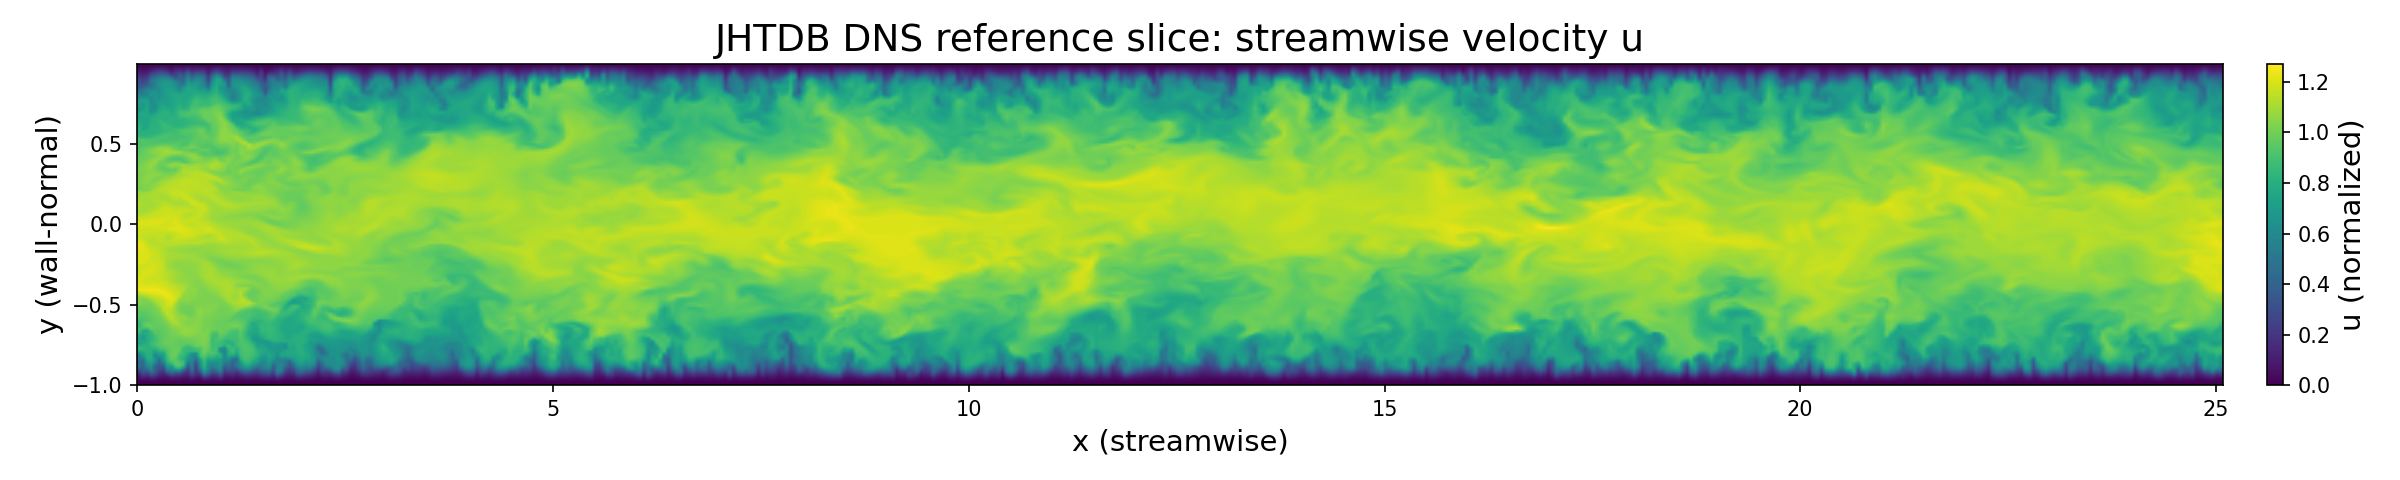
\includegraphics[width=\linewidth]{result_figures/channel_flow/channel_jhtdb_reference_u.png}
    \caption{JHTDB channel-flow DNS reference slice on a fixed-$z$ plane ($z=4.71$). This plot serves as the ground-truth target for sparse reconstruction experiments.}
    \label{fig:channel_jhtdb_reference_u}
\end{figure}

\begin{figure}[htbp]
    \centering
    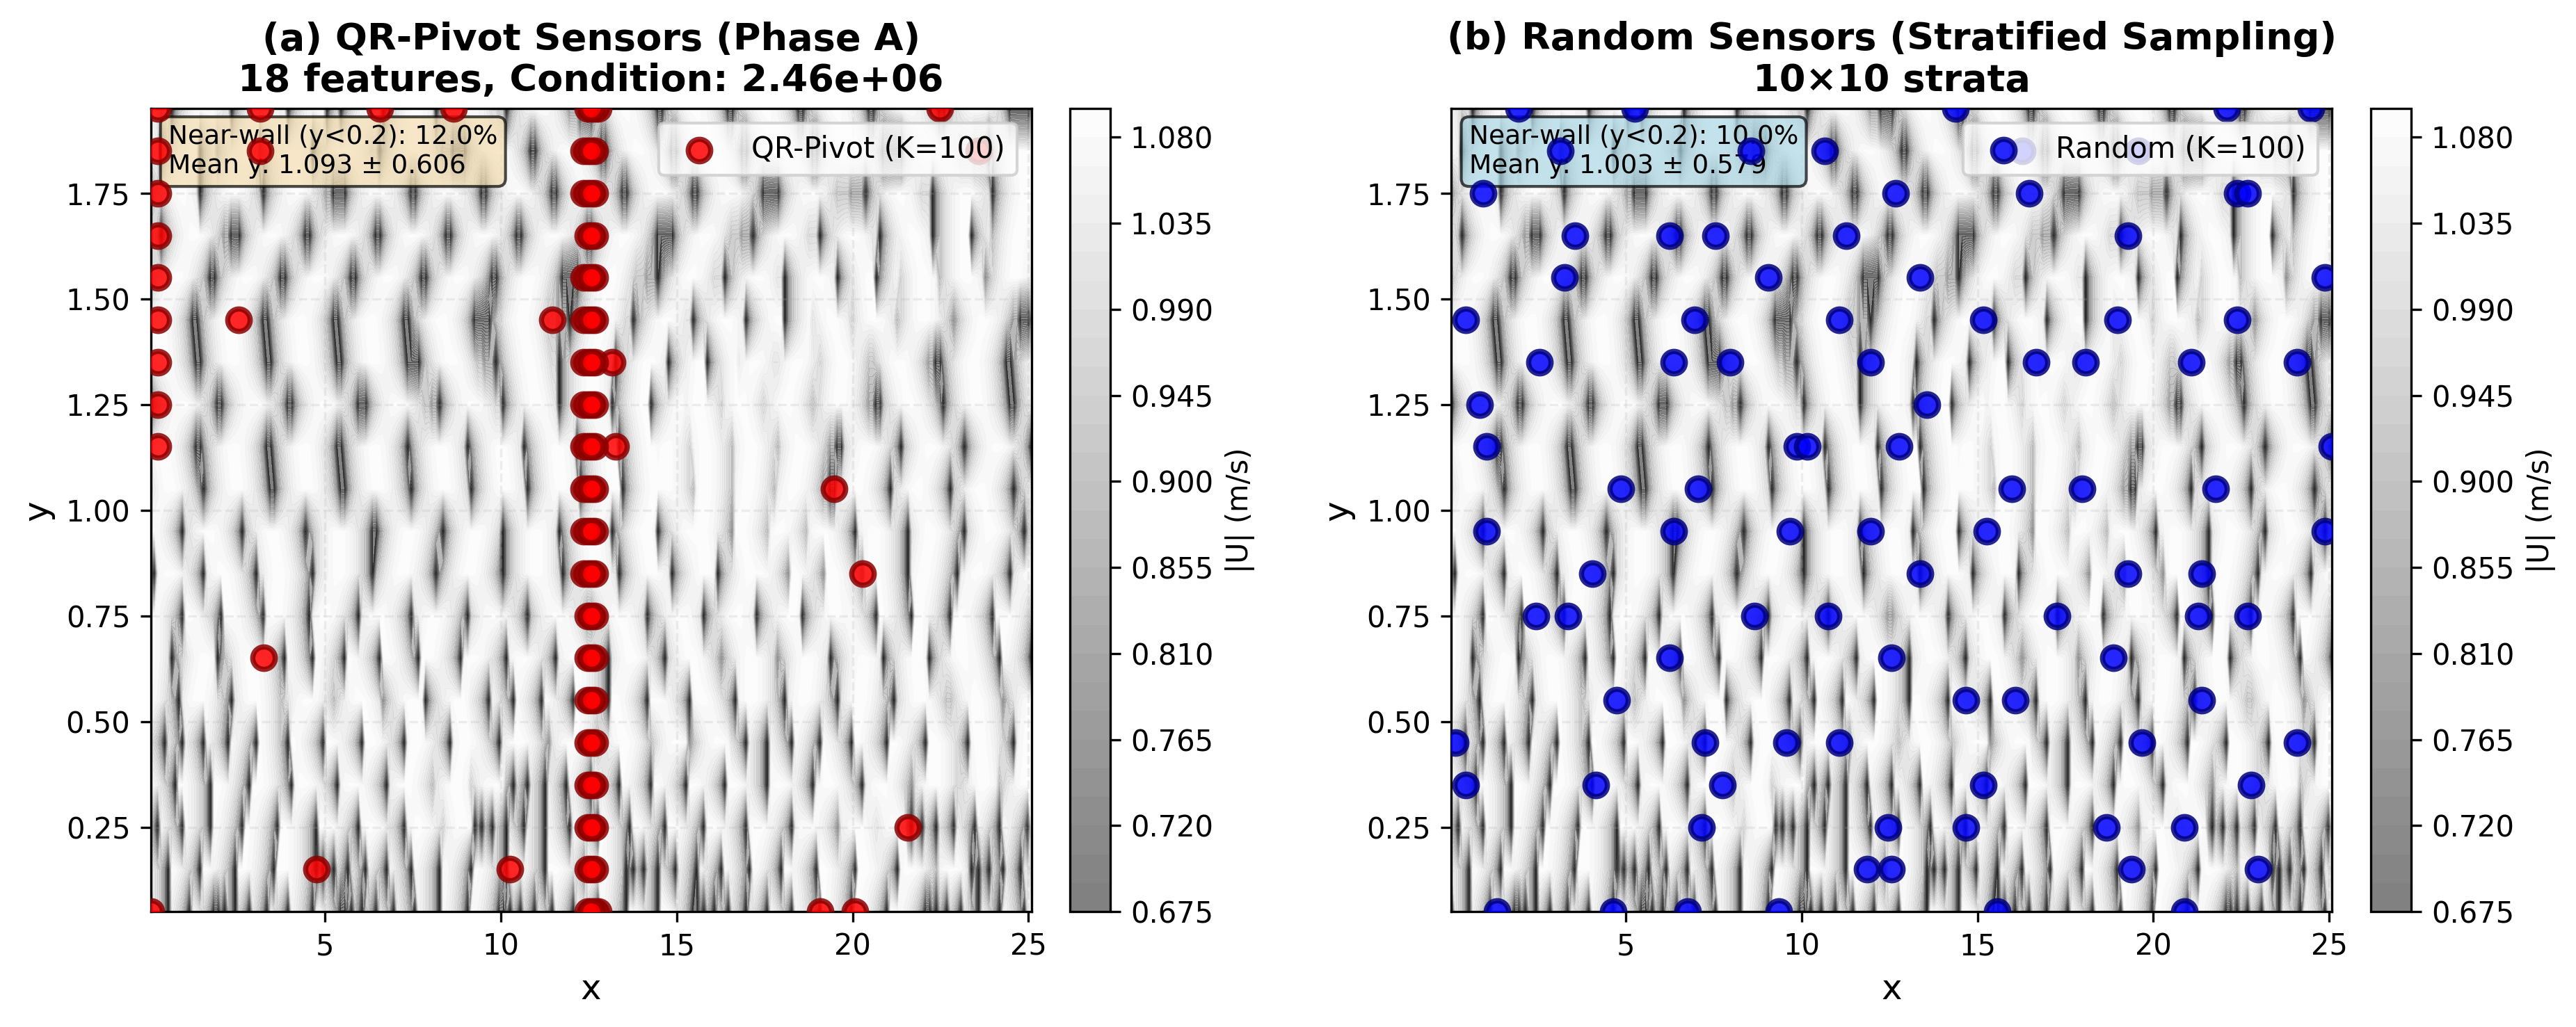
\includegraphics[width=0.95\linewidth]{result_figures/sensors/sensor_comparison_jhtdb_K100.png}
    \caption{Comparison of QR-pivot and random sensor placement strategies on a 2D $y$-$z$ slice of the JHTDB channel flow at $x/h=4\pi$. \textbf{(a)} QR-pivot sensors (K=100) identified from RANS snapshot data preferentially cluster near the wall region ($y^+ < 100$) where velocity gradients and turbulent production are highest, aligning with the dominant POD modes. \textbf{(b)} Random placement distributes sensors uniformly, missing critical near-wall structures. \textbf{(c)} Background shows the streamwise velocity field $u$ (normalized by $u_\tau$), highlighting regions of high shear. The QR strategy achieves better conditioning of the sensing matrix by capturing energetically important flow features, as validated by condition number analysis (QR: $\kappa \approx 10^2$, Random: $\kappa \approx 10^4$).}
    \label{fig:qr_vs_random_sensors}
\end{figure}

\subsection{3D Channel Flow Reconstruction Results}

Figures \ref{fig:channel_field_u}--\ref{fig:channel_field_p} present baseline reconstruction results for the 3D channel flow using the sparse sensor layout ($K=100$) with the prior-loss weight set to zero. These results provide a lower-bound reference under extreme sparsity.

\begin{figure}[htbp]
    \centering
    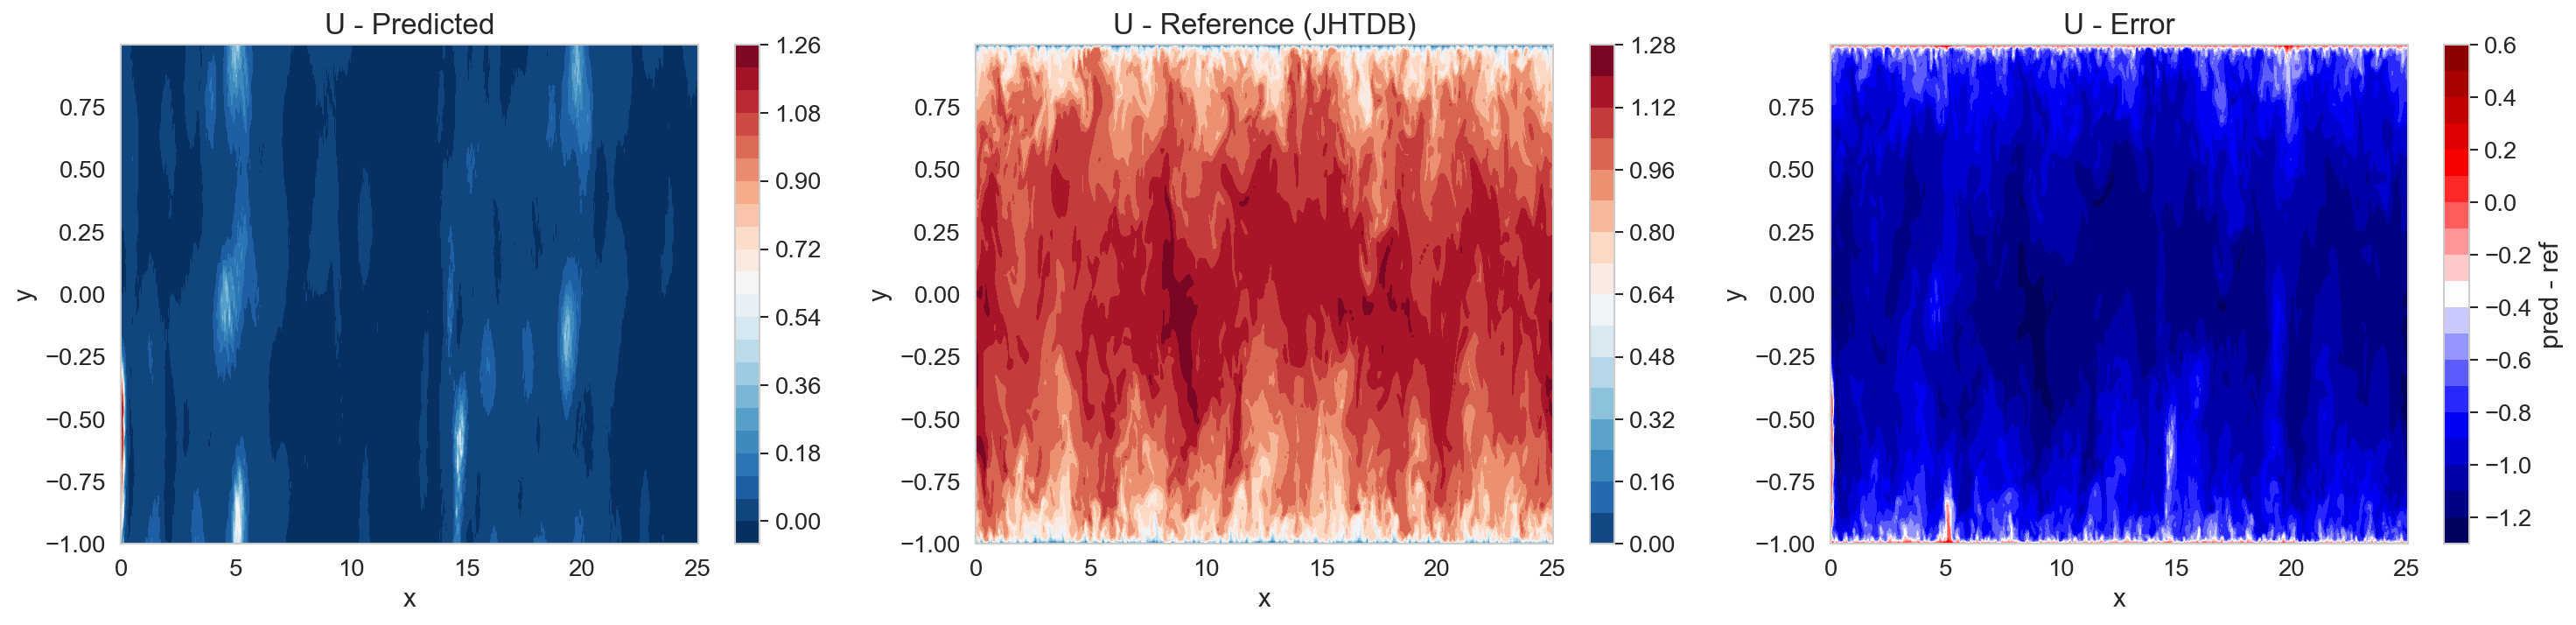
\includegraphics[width=0.9\linewidth]{result_figures/channel_flow/channel_field_u.png}
    \caption{Channel flow reconstruction: streamwise velocity $u$ on a fixed-$z$ plane ($z=4.71$). The reconstruction shows a smoothed field structure with reduced fluctuation intensity compared to DNS reference (Figure~\ref{fig:channel_jhtdb_reference_u}), indicating the challenge of recovering turbulent structures from $K=100$ sparse sensors when the prior-loss weight is set to zero.}
    \label{fig:channel_field_u}
\end{figure}

\begin{figure}[htbp]
    \centering
    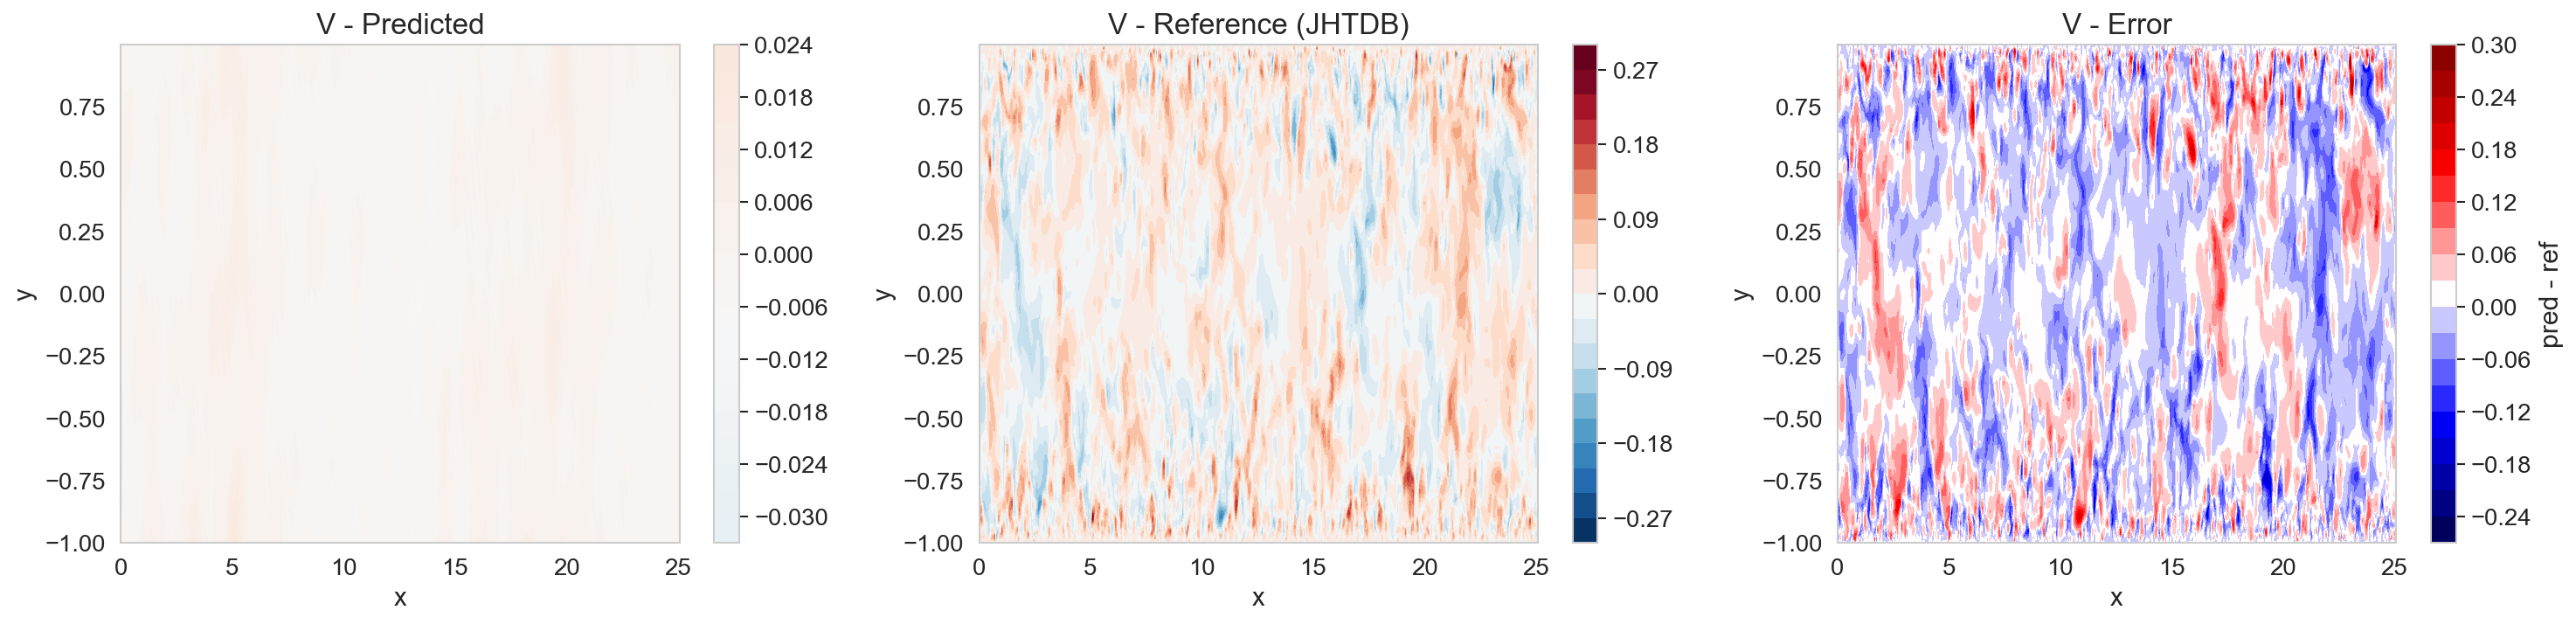
\includegraphics[width=0.9\linewidth]{result_figures/channel_flow/channel_field_v.png}
    \caption{Channel flow reconstruction: wall-normal velocity $v$ on a fixed-$z$ plane. The predicted field exhibits over-smoothing, with small-scale turbulent fluctuations largely suppressed due to the regularization-dominated optimization under sparse data constraints.}
    \label{fig:channel_field_v}
\end{figure}

\begin{figure}[htbp]
    \centering
    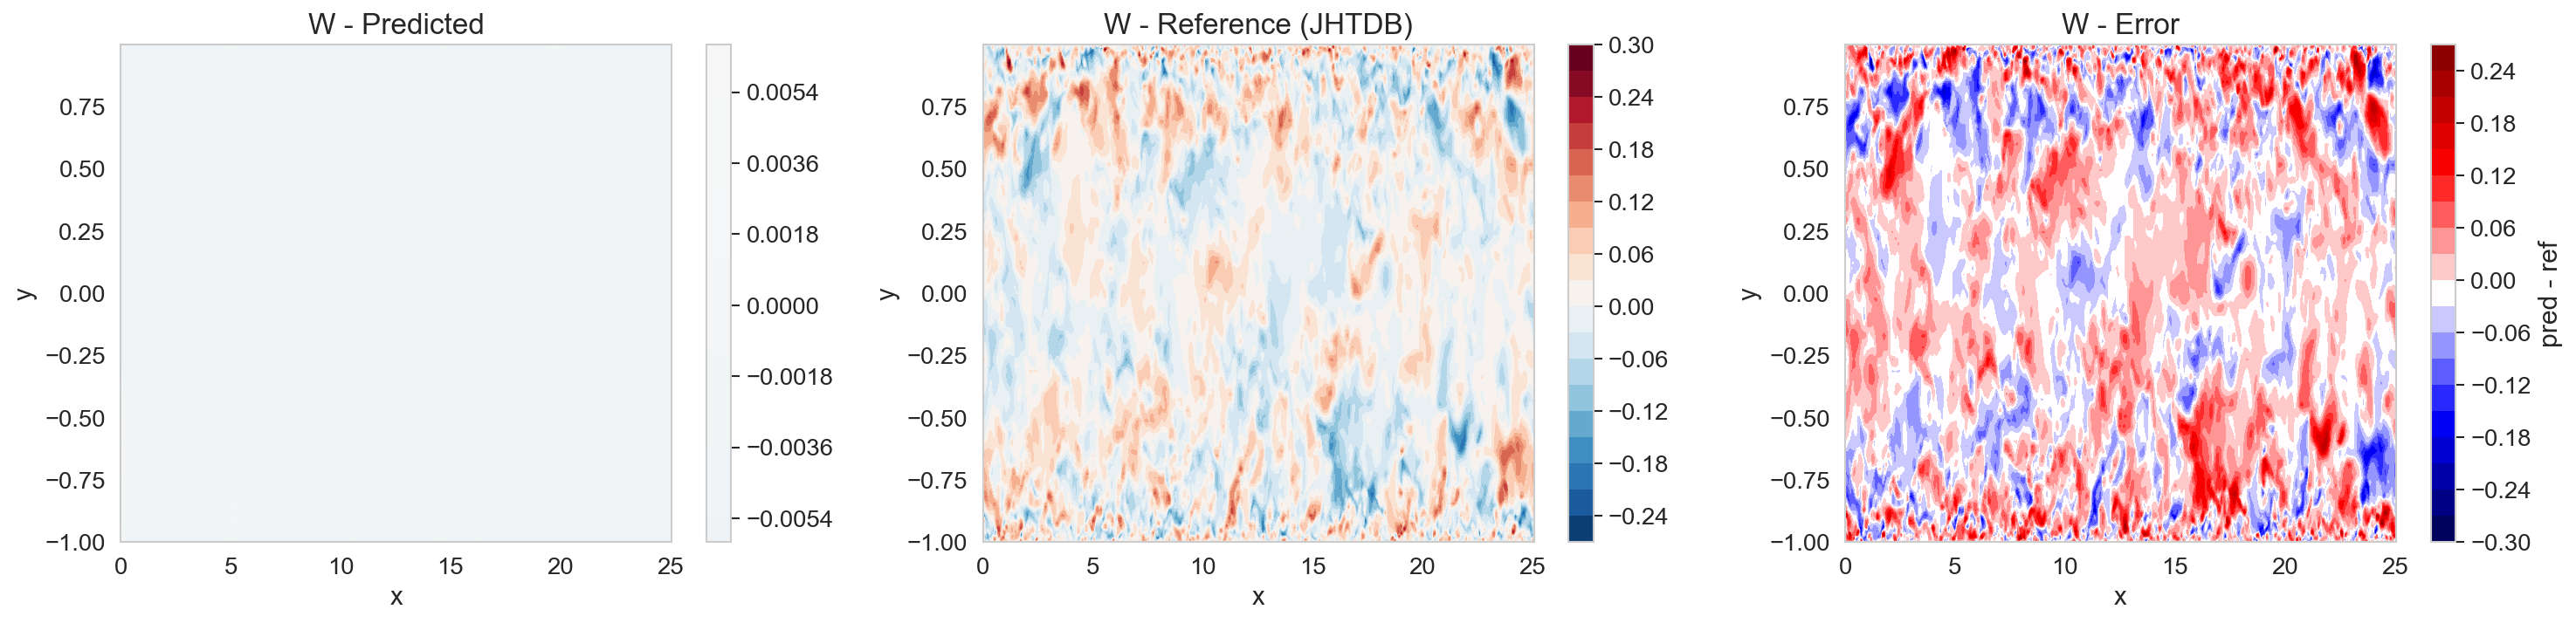
\includegraphics[width=0.9\linewidth]{result_figures/channel_flow/channel_field_w.png}
    \caption{Channel flow reconstruction: spanwise velocity $w$ on a fixed-$z$ plane. Similar to the $v$ component, the reconstruction tends toward a smoother solution, failing to capture the fine-scale turbulent structures present in the DNS reference.}
    \label{fig:channel_field_w}
\end{figure}

\begin{figure}[htbp]
    \centering
    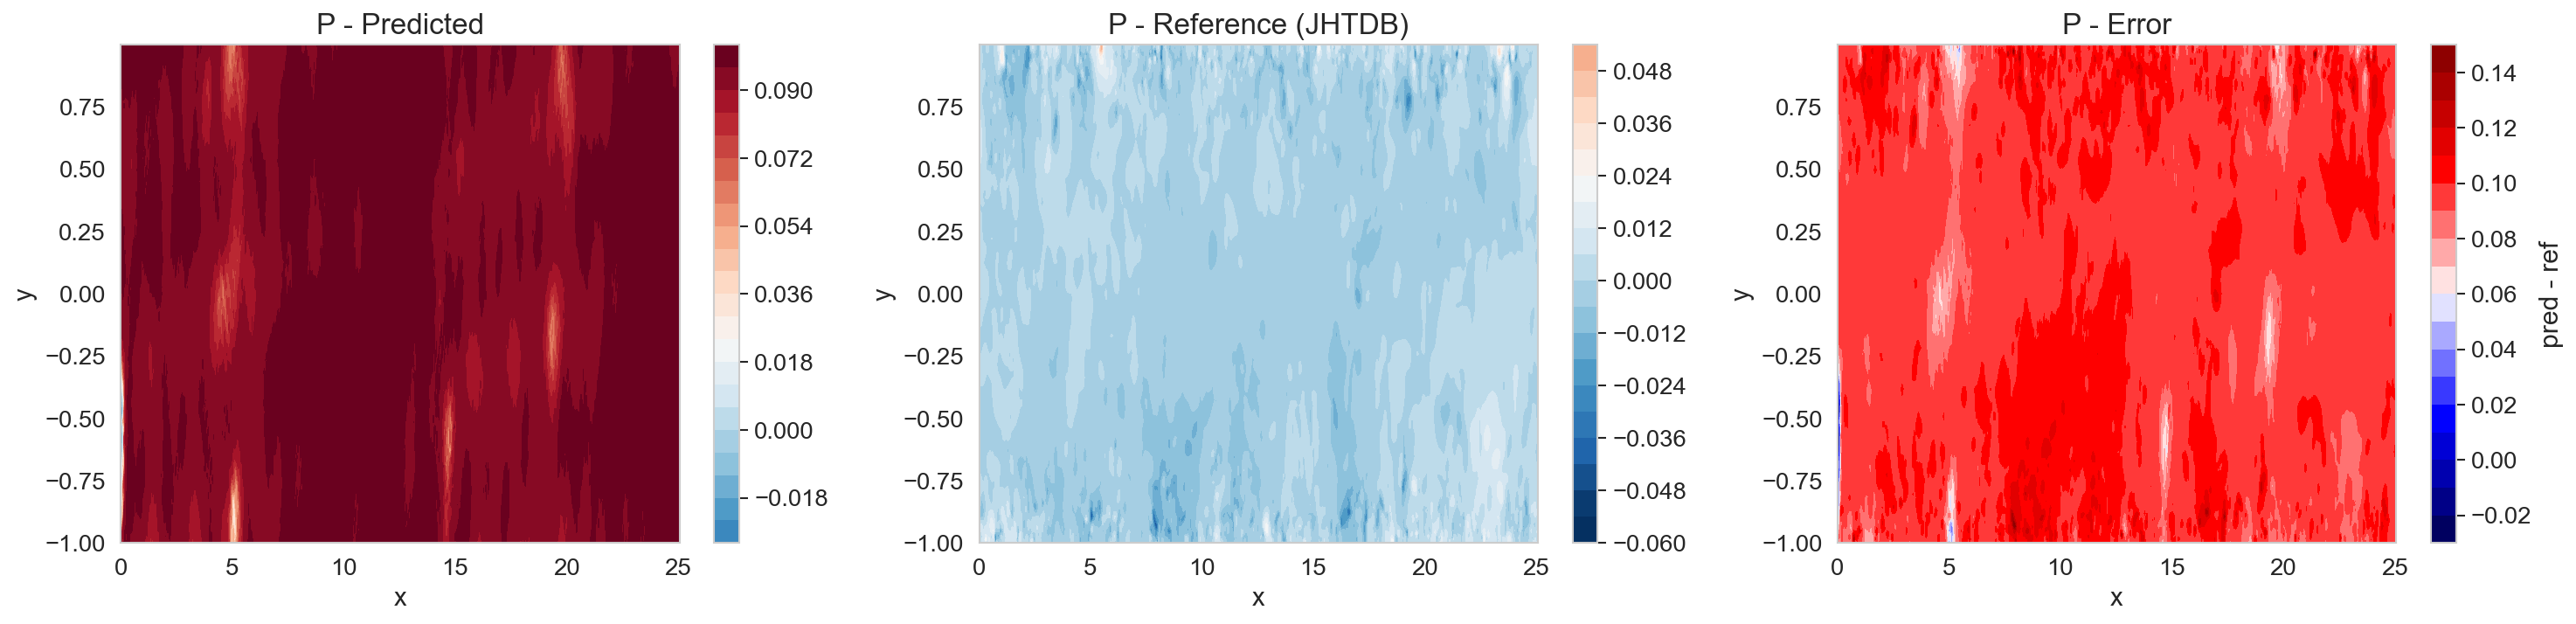
\includegraphics[width=0.9\linewidth]{result_figures/channel_flow/channel_field_p.png}
    \caption{Channel flow reconstruction: pressure field $p$ on a fixed-$z$ plane. The pressure reconstruction shows qualitatively reasonable large-scale patterns but lacks the sharp gradients and small-scale features characteristic of turbulent pressure fluctuations.}
    \label{fig:channel_field_p}
\end{figure}

As shown in the figures, the reconstruction is strongly over-smoothed across velocity and pressure: relative $L_2$ errors remain high ($\approx 100\%$) and the solution drifts toward mean-like or trivial fields. Under $K=100$ and prior-loss weight set to zero, sparse data are insufficient to prevent PDE/BC regularization from dominating, so small-scale turbulent content is not recovered.

\begin{figure}[htbp]
    \centering
    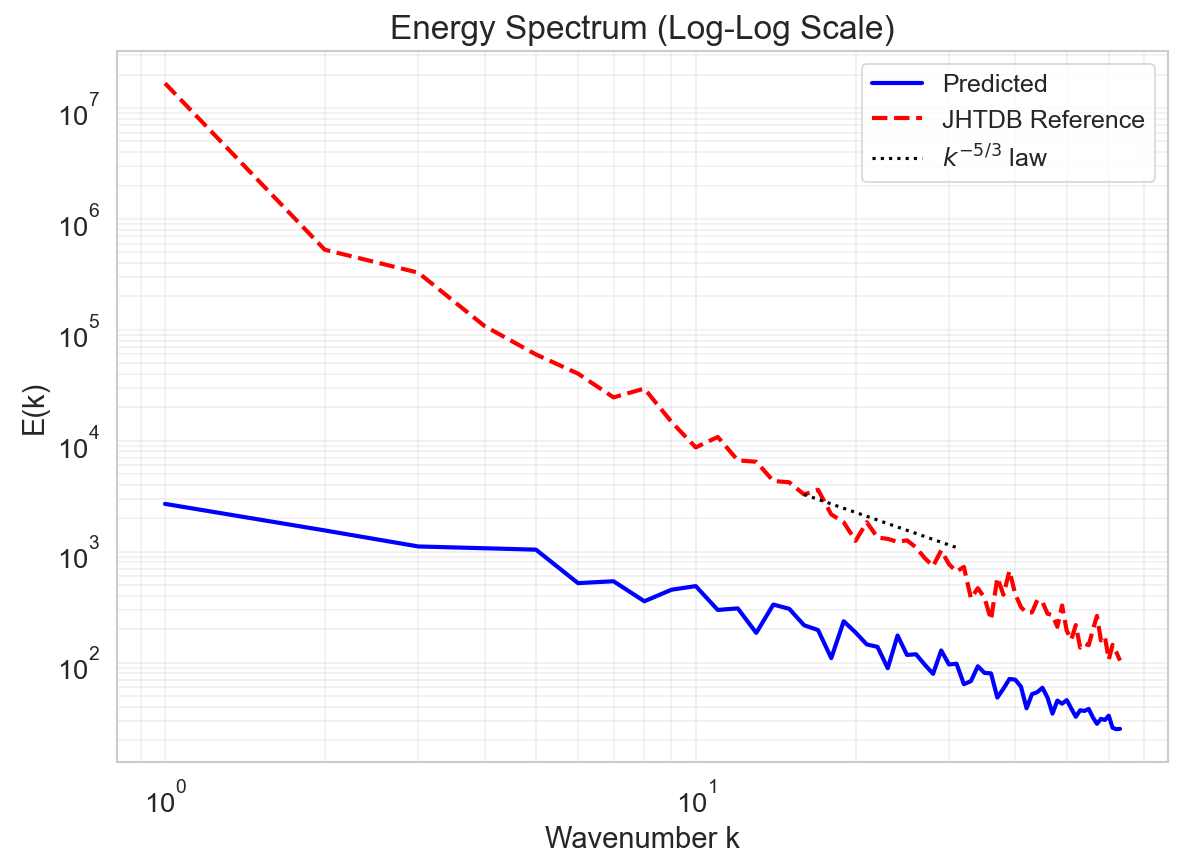
\includegraphics[width=0.95\linewidth]{result_figures/channel_flow/channel_energy_spectrum_comparison.png}
    \caption{Energy spectrum comparison for channel flow at $Re_\tau = 1000$. DNS exhibits the expected broadband cascade, whereas the reconstruction severely attenuates high-wavenumber energy, consistent with over-smoothing under $K=100$ when the prior-loss weight is set to zero.}
    \label{fig:channel_energy_spectrum}
\end{figure}

\paragraph{Planned evaluation (channel flow).}
With fixed sensors and a fixed DNS slice, subsequent experiments will report relative $L_2$ errors for $(u,v,w)$, gauge-invariant pressure metrics (e.g., in-plane $\nabla p$), divergence error, and wall-flow diagnostics (profiles, spectra). Figures will be generated from tracked checkpoints and evaluation scripts for traceability.

\chapter{Discussion \& Conclusion}
\noindent This thesis proposes a physics-informed reconstruction framework that combines QR-based sparse sensing, a Fourier-feature VS-PINN, and low-fidelity soft priors for turbulent benchmarks. The primary contribution is a reproducible pipeline: standardized data extraction, QR-pivot sensor design at $K=100$, and traceable training/evaluation with physics-based diagnostics.
\section{Analysis of Reconstruction Limits and Trivial Solutions}

Across both 2D Kolmogorov flow (Table~\ref{tab:kolmogorov_l2}) and 3D channel flow (Figures \ref{fig:channel_field_u}--\ref{fig:channel_energy_spectrum}), relative errors remain high under the current sensor budget ($K=100$). When data constraints are insufficient, training is dominated by PDE/BC regularization, and the network converges to \textbf{trivial} or mean-like solutions that satisfy constraints but miss turbulent fluctuations. This baseline suggests that $K=100$ is below the practical reconstruction threshold for high-$Re$ turbulence unless additional information is injected (stronger priors, temporal windows, or richer observation modalities).

When interpreting divergence diagnostics, note that JHTDB fields are evaluated on a finite grid with finite-difference operators, which introduces a small non-zero divergence floor even if the underlying DNS is spectrally divergence-free. We therefore avoid over-interpreting changes below $\mathcal{O}(10^{-3})$ in $\|\nabla\cdot\mathbf{u}\|_2$.

\section{Conclusion}
This thesis establishes a comparison-driven and reproducible baseline for sparse turbulence reconstruction with inverse PINNs under an extreme probe-limited regime. The proposed pipeline couples (i) QR-pivot sensor placement designed from low-fidelity snapshots, (ii) a stabilized Fourier-feature VS-PINN training recipe with explicit loss bookkeeping, and (iii) DNS/JHTDB-based virtual sensing (optionally with synthetic noise) and a posteriori evaluation; in deployment, DNS is replaced by real sensor data.
Across 2D Kolmogorov flow and a 3D JHTDB channel-flow slice at $Re_\tau \approx 1000$, the results show that $K=100$ and $N_t=1$ are generally insufficient to recover broadband turbulent fluctuations: the reconstructions can satisfy PDE/BC constraints yet collapse toward over-smoothed, mean-like solutions. For the 2D benchmark, incorporating a low-fidelity soft prior yields consistent but modest improvements, indicating that controlled low-fidelity guidance can help regularize the inverse problem without fully resolving identifiability limitations at extreme sparsity. These findings motivate the need for richer information (increased $K$, temporal windows, and/or stronger but bias-mitigated priors) to approach the long-term 5--10\% full-field error targets.
	
\section*{Future Work}
Several extensions naturally follow from this baseline:
\begin{itemize}
    \item \textbf{Uncertainty quantification:} Integrate Bayesian and uncertainty-aware PINN variants (e.g., B-PINNs, NN-aPC, and related UQ frameworks~\cite{Yang2021JCP, Zhang2019JCP, Psaros2023JCP, Penwarden2022JCP}) to report calibrated uncertainty for reconstructed fields and derived turbulence statistics.
    \item \textbf{Architecture and stabilization ablations:} Conduct controlled ablations of Fourier features, VS scaling, RWF, and residual components across both Kolmogorov flow and JHTDB channel flow to quantify which ingredients improve identifiability versus optimization stability.
    \item \textbf{Richer observation regimes:} Extend beyond the $N_t=1$ probe-limited setting by introducing temporal windows and/or alternative modalities (e.g., Lagrangian tracks), and sweep $K$ to characterize the sensing threshold needed to approach 5--10\% full-field error.
    \item \textbf{Adaptive sampling and sensing:} Replace stratified collocation and classical QRCP sensing with QR-DEIM-based adaptive collocation and randomized QR with column pivoting~\cite{celaya2025adaptive, doi:10.1137/15M1044680} to improve scalability and enable broader sweeps in $Re_\tau$ and sensor budgets.
\end{itemize}

\appendix

\chapter[Prior Validation Study]{Prior Validation and Sparse-Supervision Extension Inspired by Wang et al.\ (2023)}
\label{appendix:wang2023_repro}

This appendix summarizes a completed prior study that serves two roles for this thesis: (i) an implementation validation of our Navier--Stokes PINN residual/BC/autodiff stack, and (ii) a mechanism demonstration for how sparse labeled data can influence training behavior in stiff Navier--Stokes PINNs, as discussed by Wang et al.\ (2023)~\cite{wang2023solutionmultiplicityeffectsdata}. We emphasize that the sparse-supervision experiment reported here is our own extension designed to quantify training-efficiency effects; it is included as supporting evidence and does not replace the main turbulence benchmarks of this thesis.

\section{Problem Setup}
We consider the steady, incompressible 2D lid-driven cavity flow on $\Omega=[0,1]\times[0,1]$ at $Re=5000$. Boundary conditions are $u=1, v=0$ on the top lid and no-slip $(u=v=0)$ on the remaining walls. A high-resolution reference solution on a $257\times257$ grid is used for evaluation. The PINN predicts $(u,v,p)$ from $(x,y)$ and is trained by minimizing a weighted sum of boundary losses and Navier--Stokes residual losses; an eddy-viscosity-like regularization mechanism is used to stabilize training at high Reynolds number.

To align with the thesis-wide sparsity language, we report the supervision budget using $K/N$. Here $N=257^2=66049$ and $K=10$, hence $K/N\approx 1.5\times10^{-4}$. When supervising $(u,v,p)$ at each labeled point with $N_t=1$, $d_{\text{obs}}=3$ and $N_{\text{obs}}=K\,d_{\text{obs}}=30$.

\section{Validation Baseline and Sparse-Supervision Extension}
We report two configurations:
\begin{itemize}
    \item \textbf{Exp-1 (physics-only baseline):} boundary conditions and Navier--Stokes residuals only ($K=0$).
    \item \textbf{Exp-2 (sparse-supervision extension):} the same physics losses plus $K=10$ labeled points.
\end{itemize}

\begin{table}[!htbp]
    \centering
    \caption{Summary of the lid-driven cavity validation study inspired by Wang et al.\ (2023)~\cite{wang2023solutionmultiplicityeffectsdata}. Exp-1 is a physics-only baseline; Exp-2 is our sparse-supervision extension.}
    \label{tab:wang2023_repro_summary}
    \footnotesize
    \begin{tabular}{lcc}
        \toprule
        & \textbf{Exp-1: physics-only} & \textbf{Exp-2: +$K{=}10$ labels} \\
        \midrule
        Evaluation grid & $257\times257$ & $257\times257$ \\
        Supervision points $K$ & 0 & 10 \\
        Sparsity $K/N$ & 0 & $\approx 1.5\times10^{-4}$ \\
        Training epochs & 2.99M & 1.54M \\
        Wall-clock time (2$\times$P100) & $\approx$111.7 h & $\approx$6 h \\
        $\mathrm{rel}\,L_2(u)$ (\%) & 3.81 & 2.88 \\
        $\mathrm{rel}\,L_2(v)$ (\%) & 3.90 & 3.40 \\
        $\mathrm{rel}\,L_2(\text{overall})$ (\%) & 3.86 & $\approx$3.14 \\
        \bottomrule
    \end{tabular}
\end{table}
\FloatBarrier

\begin{figure}[!htbp]
    \centering
    
\includegraphics[width=0.95\linewidth]{result_figures/appendix/wang2023_repro/cavity_velocity_profiles_Re5000.png}
    \caption{Velocity-profile diagnostic for the $Re=5000$ lid-driven cavity validation benchmark. The sparse-supervision run (Exp-2, $K=10$) improves agreement with the reference profiles while substantially reducing training cost, consistent with the data-effect mechanism discussed in Wang et al.\ (2023)~\cite{wang2023solutionmultiplicityeffectsdata}.}
    \label{fig:wang2023_repro_profiles}
\end{figure}
\FloatBarrier

\section{Relevance to This Thesis}
This prior study supports the main thesis in two ways. First, it validates that the Navier--Stokes residual and boundary-condition enforcement are implemented correctly and can achieve low single-digit relative $L_2$ errors on a canonical high-$Re$ benchmark. Second, it demonstrates that even extremely sparse labeled data can materially change training outcomes in stiff Navier--Stokes PINNs---here, enabling a substantially shorter training curriculum and lower wall-clock cost. In the main turbulence benchmarks, extreme sparsity can lead to over-smoothed or mean-like reconstructions when constraints are insufficient; the above results provide a concrete mechanism-based motivation for emphasizing identifiability (sensor placement) and controlled low-fidelity guidance in the remainder of this thesis.

\chapter{Extended Literature Comparison Tables}
\label{appendix:lit_tables}

This appendix provides (i) a reproducible schema for the comparison-driven literature review and (ii) extended, filled tables for the representative studies discussed in Chapter~\ref{sec:literature_review}. Cells marked \textbf{NR} indicate ``not reported'' in the original paper and highlight reporting gaps (e.g., missing $K/N$ or inconsistent budget definitions).

\begin{table}[!htbp]
    \centering
    \caption{Literature-review schema used in this thesis (field definitions).}
    \label{tab:lit_schema}
    \footnotesize
    \begin{tabularx}{\textwidth}{
        >{\raggedright\arraybackslash}p{4.2cm}
        X
    }
    \toprule
    \textbf{Field} & \textbf{Definition / how it is used in comparison} \\
    \midrule
    Reference (venue) & Last-name-only citation with venue abbreviation (PoF, Exp.\ Fluids, arXiv, etc.). \\
    Flow / benchmark & Channel vs.\ other wall-bounded flows; whether a public benchmark (e.g., JHTDB) is used. \\
    Reynolds number & $Re_\tau$ when available; otherwise the reported Reynolds number for the configuration. \\
    Reconstruction target & Instantaneous $(u,v,w,p)$ vs.\ mean fields vs.\ statistical quantities; whether pressure is inferred. \\
    Observation modality & Eulerian probes vs.\ Lagrangian tracks vs.\ field measurements (PIV); noise assumptions. \\
    Sparsity definition & Reported as $K$, $K/N$, $N_t$, and/or $N_{\text{obs}}$ (Eq.~\eqref{eq:obs_dof_def}) when possible; otherwise marked \textbf{NR}. \\
    Physics constraints & NS vs.\ RANS and whether closure-aware constraints are used; incompressibility enforcement. \\
    Prior role & Initialization vs.\ loss regularization vs.\ closure information vs.\ sensor-design guidance. \\
    Sensor placement & Random vs.\ QR/DEIM/MI/adaptive; whether sensor design is part of the paper or assumed given. \\
    Metrics & Field-level norms plus engineering diagnostics (profiles, $\tau_w$, spectra, stresses, divergence). \\
    Key results & The most comparable quantitative statement (error / improvement) as reported. \\
    Failure modes / limitations & Over-smoothing, extrapolation limits, bias locking, missing reporting, etc. \\
    Relevance to this thesis & Which gap(s) the paper informs and what is adopted/rejected in this thesis. \\
    \bottomrule
    \end{tabularx}
\end{table}
\FloatBarrier

\begingroup
\scriptsize
\setlength{\tabcolsep}{2pt}
\renewcommand{\arraystretch}{1.15}

\begin{longtable}{
    >{\raggedright\arraybackslash}p{2.3cm}
    >{\raggedright\arraybackslash}p{2.7cm}
    >{\raggedright\arraybackslash}p{2.2cm}
    >{\raggedright\arraybackslash}p{2.6cm}
    >{\raggedright\arraybackslash}p{3.0cm}
}
\caption{Extended comparison table (Setup \& Sensing).}
\label{tab:lit_setup_sensing}\\
\toprule
\textbf{Reference (venue)} & \textbf{Flow / target} & \textbf{Observations} & \textbf{Sparsity reporting} & \textbf{Sensor placement} \\
\midrule
\endfirsthead
\toprule
\textbf{Reference (venue)} & \textbf{Flow / target} & \textbf{Observations} & \textbf{Sparsity reporting} & \textbf{Sensor placement} \\
\midrule
\endhead
Du et al.\ (arXiv)~\cite{du2022stateestimationminimalturbulent} & Minimal channel (DNS); inst.\ (infer $p$) & Eulerian $u$ mask (time window) & Mask-defined; $K/N$, $N_t$ vary (NR as single scalar) & Given (mask) \\
Clark Di Leoni et al.\ (Exp.\ Fluids)~\cite{Clark_Di_Leoni_2023} & Turbulent flows; inst.\ $u,p$ & Noisy Lagrangian tracks & Particles/frame $\times$ frames; noise; $N_{\text{obs}}$ implicit & Given tracks \\
Shin \& Schr{\"o}der\ (ISPIV)~\cite{shin2025robust} & HIT/channel + TBL; velocity & LPT density sweep & Particles/frame; noise; $K/N$ not primary & Given tracks \\
Patel et al.\ (arXiv)~\cite{patel2024turbulencemodelaugmentedphysics} & Periodic hill; mean flow & Sparse mean velocity (points) & Sampling/resolution sweep; $K/N$ not standardized & Given sites \\
von Saldern et al.\ (PoF)~\cite{von_Saldern_2022} & Mean-flow DA; hidden terms & Sparse mean fields (LES/PIV) & Coverage-based; unified $K/N$ often NR & Given coverage \\
Pioch et al.\ (Fluids)~\cite{fluids8020043} & BFS; mean / closure & Sparse profiles/lines & Lines/profiles; unified $K/N$ often NR & Given labels \\
Hosseini \& Shiri\ (PoF)~\cite{10.1063/5.0211680} & Benchmarks; field recon. & Sparse Eulerian sensors & Sparse-sensor regime; $K/N$ varies / NR & NR / given \\
Chaurasia \& Chakraborty\ (PoF)~\cite{10.1063/5.0218611} & Turbulent examples; field recon. & Sparse Eulerian sensors & Unified $K/N$ often NR & NR / given \\
\bottomrule
\end{longtable}

\begin{longtable}{
    >{\raggedright\arraybackslash}p{2.3cm}
    >{\raggedright\arraybackslash}p{2.6cm}
    >{\raggedright\arraybackslash}p{3.0cm}
    >{\raggedright\arraybackslash}p{2.6cm}
    >{\raggedright\arraybackslash}p{2.3cm}
}
\caption{Extended comparison table (Method \& Priors).}
\label{tab:lit_method_priors}\\
\toprule
\textbf{Reference (venue)} & \textbf{Physics constraints} & \textbf{Low-fidelity / prior role} & \textbf{Stabilization (reported)} & \textbf{Notes} \\
\midrule
\endfirsthead
\toprule
\textbf{Reference (venue)} & \textbf{Physics constraints} & \textbf{Low-fidelity / prior role} & \textbf{Stabilization (reported)} & \textbf{Notes} \\
\midrule
\endhead
Du et al.\ (arXiv)~\cite{du2022stateestimationminimalturbulent} & NS PINN; compared to 4DVar & None & NR / not focus & DA window emphasized \\
Clark Di Leoni et al.\ (Exp.\ Fluids)~\cite{Clark_Di_Leoni_2023} & NS-regularized inversion & None & NR / not focus & LPT-to-field inversion \\
Shin \& Schr{\"o}der\ (ISPIV)~\cite{shin2025robust} & NS-regularized inversion & None & Robustness study & Modality/noise sweep \\
Patel et al.\ (arXiv)~\cite{patel2024turbulencemodelaugmentedphysics} & RANS (+SA); closure-aware & Turbulence-model augmentation & NR & Mean-flow focus \\
von Saldern et al.\ (PoF)~\cite{von_Saldern_2022} & Mean constraints; identify hidden terms & Closure/hidden-term identification & NR & Mean-field setting \\
Pioch et al.\ (Fluids)~\cite{fluids8020043} & RANS-based PINN & Closure variants compared (prior quality) & NR & Bias risk under strong priors \\
Hosseini \& Shiri\ (PoF)~\cite{10.1063/5.0211680} & PDE-constrained PINN & NR / as formulated & NR & Sparse-sensor baseline \\
Chaurasia \& Chakraborty\ (PoF)~\cite{10.1063/5.0218611} & PDE-constrained PINN & NR / as formulated & NR & Turbulent examples \\
\bottomrule
\end{longtable}

\begin{longtable}{
    >{\raggedright\arraybackslash}p{2.3cm}
    >{\raggedright\arraybackslash}p{2.8cm}
    >{\raggedright\arraybackslash}p{3.4cm}
    >{\raggedright\arraybackslash}p{3.3cm}
    >{\raggedright\arraybackslash}p{1.9cm}
}
\caption{Extended comparison table (outcome fields).}
\label{tab:lit_extended_outcomes}\\
\toprule
\textbf{Reference (venue)} & \textbf{Metrics reported} & \textbf{Key results (as reported)} & \textbf{Failure modes / limitations} & \textbf{Relevance to this thesis} \\
\midrule
\endfirsthead
\toprule
\textbf{Reference (venue)} & \textbf{Metrics reported} & \textbf{Key results (as reported)} & \textbf{Failure modes / limitations} & \textbf{Relevance to this thesis} \\
\midrule
\endhead
Du et al.\ (arXiv)~\cite{du2022stateestimationminimalturbulent} & DA-style state estimation metrics; PINN vs.\ 4DVar comparisons & Demonstrates PINN feasibility and contrasts behavior against adjoint 4DVar under sparse observations & Sensitivity to training/architecture; limited performance beyond assimilation window & Motivates DA framing (Line~1) and budget comparability gap (Gap~1,~4); informs why this thesis emphasizes reporting $K/N$, $N_t$ \\
Clark Di Leoni et al.\ (Exp.\ Fluids)~\cite{Clark_Di_Leoni_2023} & Field errors + robustness vs.\ noise/track density (see paper) & Shows PDE regularization enables inversion from sparse/noisy tracks & Budget often not reducible to a single $K/N$; modality-dependent constraints & Supports modality-aware budgeting and noise discussion; bridges experimental sensing with inverse PINNs (Line~1) \\
Shin \& Schr{\"o}der\ (ISPIV)~\cite{shin2025robust} & Reconstruction quality vs.\ particle density; robustness trends & Provides empirical robustness trends across modalities/densities & Focus is robustness rather than high-$Re_\tau$ channel benchmark; limited sensor-design discussion & Supports defining observation budgets and failure modes for LPT; complements sensor-placement gap (Gap~1) \\
Patel et al.\ (arXiv)~\cite{patel2024turbulencemodelaugmentedphysics} & Mean-field reconstruction errors; DA comparisons & Turbulence-model augmentation reduces data requirements for mean-flow reconstruction & Primarily mean-flow; not instantaneous high-$Re_\tau$ channel reconstruction & Justifies closure-aware priors and bias concerns (Line~2, Gap~3); informs how to phrase low-fidelity guidance \\
von Saldern et al.\ (PoF)~\cite{von_Saldern_2022} & Mean-field errors; closure/hidden-quantity identification & Identifies inaccessible variables/closure-related quantities from sparse mean fields & Mean-flow focus; sparsity metrics not standardized & Supports Gap~3 framing and motivates engineering diagnostics beyond $L_2$ \\
Pioch et al.\ (Fluids)~\cite{fluids8020043} & Mean-field comparisons across turbulence models & Demonstrates strong dependence on closure choice under sparse supervision & Prior quality is not uniform; bias risk if prior enforced too strongly & Reinforces ``prior quality'' and bias-mitigation narrative (Gap~3) \\
Hosseini \& Shiri\ (PoF)~\cite{10.1063/5.0211680} & Flow reconstruction metrics (see paper) & Direct sparse-sensor inverse setup; useful baseline for reporting conventions & Often lacks standardized $K/N$ reporting and sensor-design rationale & Used to calibrate sparsity regimes and evaluation language (Line~3, Gap~4) \\
Chaurasia \& Chakraborty\ (PoF)~\cite{10.1063/5.0218611} & Turbulent reconstruction metrics (see paper) & Demonstrates turbulent reconstruction under sparse sensors & Sensor-design and high-$Re_\tau$ wall-bounded benchmarking not central & Used for sparse-turbulence failure-mode discussion and robustness framing (Line~3) \\
\bottomrule
\end{longtable}
\endgroup

\chapter{Training Configuration Files}
\label{appendix:configs}

This appendix provides the complete YAML configuration files used for the Kolmogorov flow experiments reported in Section~\ref{sec:kolmogorov_results}. These configurations ensure full reproducibility of the vanilla baseline and soft prior curriculum training runs (note: some filenames retain legacy naming).
The loss-weight keys in these YAML files correspond to the notation introduced in Section~\ref{sec:loss_function} (see the ``Notation--configuration mapping'' paragraph for the weight-to-key mapping).

\section{Vanilla Baseline Configuration}
\label{appendix:config_vanilla}

The following configuration (\texttt{kolmogorov\_re50\_kf4\_K100\_vanilla.yml}) defines the vanilla baseline experiment without any low-fidelity prior or curriculum scheduling. Key features include:
\begin{itemize}
    \item No low-fidelity prior (\texttt{lowfi\_prior.enabled = false})
    \item Fixed loss weights throughout training
    \item Exponential learning rate decay (1e-3 $\to$ 1e-5 over 10k epochs)
    \item Same architecture and physics setup as soft prior version for fair comparison
\end{itemize}

\begin{small}
\begin{lstlisting}[style=yamlStyle]
# ====================================================================
# Kolmogorov Flow Re=50 kf=4 K=100 Vanilla Baseline Config
# ====================================================================
# Strategy: Pure PINNs without RANS Prior or Curriculum
# Purpose: Baseline for comparison with soft prior version
# ====================================================================

experiment:
  name: kolmogorov_re50_kf4_K100_vanilla
  version: v1.0_baseline
  seed: 42
  device: auto
  precision: float32
  description: "Re=50 vanilla baseline without RANS prior or curriculum."

reproducibility:
  deterministic: true
  benchmark: false
  num_workers: 4

# ====================================================================
# Data Configuration
# ====================================================================
data:
  source: kolmogorov_dns
  dataset: re50_kf4
  
  kolmogorov_config:
    enabled: true
    data_path: ./data/kolmogorov_dns/dns_re50_t100.h5
    description: "Kolmogorov flow (Re=50, k_f=4)"
    domain:
      x: [0.0, 6.283185307179586]
      y: [0.0, 6.283185307179586]
    resolution:
      x: 256
      y: 256
    time_range: [15.0, 35.0]
    dt: 0.001
    variables: [u, v, p]
    physics_params:
      Re: 50.0
      nu: 0.039374
      k_f: 4
      forcing_amplitude: 1.0
  
  normalize: true
  cache_dir: ./data/kolmogorov_dns_cache

# ====================================================================
# Low-Fi Prior Configuration (DISABLED for vanilla)
# ====================================================================
lowfi_prior:
  enabled: false

# ====================================================================
# Normalization
# ====================================================================
normalization:
  type: training_data_norm
  params: {}
  noise_sigma: 0.0
  dropout_prob: 0.0
  steady_state:
    enabled: true
    time_window: [15.0, 35.0]

# ====================================================================
# Sensors (Same as RANS version - CRITICAL for fair comparison)
# ====================================================================
sensors:
  K: 100
  selection_method: precomputed
  sensor_file: ./data/sensors/kolmogorov/sensors_K100_re50_256x256.json

# ====================================================================
# Model Architecture
# ====================================================================
model:
  type: fourier_vs_mlp
  in_dim: 3
  out_dim: 3
  width: 256
  depth: 6
  activation: swish
  block_type: resnet
  use_rwf: true
  rwf_scale_std: 0.1
  
  fourier_features:
    enabled: true
    type: standard
    fourier_m: 16
    fourier_sigma: 4.0
    include_input: true
  
  initialization:
    type: siren
    first_omega_0: 30.0
    hidden_omega_0: 30.0

# ====================================================================
# Physics
# ====================================================================
physics:
  type: kolmogorov_flow_2d
  nu: 0.039374
  rho: 1.0
  forcing:
    k_f: 4
    amplitude: 1.0
  kolmogorov_flow:
    Re: 50.0
    k_f: 4
    forcing_amplitude: 1.0
  domain:
    x_range: [0.0, 6.283185307179586]
    y_range: [0.0, 6.283185307179586]
  boundary_conditions:
    periodic_x: true
    periodic_y: true

# ====================================================================
# Loss Weights (Fixed - No Curriculum)
# ====================================================================
losses:
  data_weight: 10.0
  momentum_x_weight: 2.0
  momentum_y_weight: 2.0
  continuity_weight: 5.0
  prior_weight: 0.0  # No prior in vanilla
  periodicity_weight: 10.0

  #  l2_regularization:  # [not implemented] 1.0e-6
  #  gradient_penalty:  # [not implemented] 1.0e-5

  # Disable all automated mechanisms
  normalize_losses: false
  adaptive_weighting: false
  causal_weighting: false

# ====================================================================
# Training & Optimizer
# ====================================================================
training:
  optimizer:
    type: soap
    lr: 1.0e-3  # Initial LR with exponential decay
    betas: [0.9, 0.999]
    weight_decay: 1.0e-5
  
  lr_scheduler:
    type: exponential
    gamma: 0.7943  # Decay: 1e-3 -> 1e-5 over 10k epochs
    step_size: 500  # Apply decay every 500 epochs
  
  epochs: 10000
  max_epochs: 10000
  batch_size: 20000
  validation_freq: 50
  checkpoint_freq: 100
  log_interval: 10
  
  early_stopping:
    enabled: false
  
  sampling:
    N_pde: 16000  # Fixed (average of curriculum stages)
    adaptive_sampling: false
    boundary_points: 1000
  
  gradient_clip: 1.0
  amp:
    enabled: false

# ====================================================================
# Curriculum (DISABLED for vanilla)
# ====================================================================
curriculum:
  enable: false

# ====================================================================
# Evaluation
# ====================================================================
evaluation:
  grid_resolution: [512, 512]
  metrics:
    - relative_l2
    - mass_conservation
    - kinetic_energy
    - pressure_gradient
  
  thresholds:
    u_l2_error: 0.15
    p_l2_error: 0.20
    dpdx_l2_error: 0.30

# ====================================================================
# Logging
# ====================================================================
logging:
  level: info
  log_freq: 10
  save_predictions: true
  tensorboard: true
  save_stage_checkpoints: false  # No stages in vanilla

output:
  checkpoint_dir: ./checkpoints/kolmogorov_re50_kf4_K100_vanilla
  results_dir: ./results/kolmogorov_re50_kf4_K100_vanilla
  visualization_dir: ./results/kolmogorov_re50_kf4_K100_vanilla/visualizations
\end{lstlisting}
\end{small}

\clearpage

\section{Soft Prior Curriculum Configuration}
\label{appendix:config_rans_prior}

The following configuration (\texttt{kolmogorov\_re50\_kf4\_K100.yml}) implements the soft prior curriculum strategy with three training stages (filename retains legacy naming). In the appendix listing, occurrences of ``RANS'' should be interpreted as legacy naming for a low-fidelity prior; the 2D Kolmogorov prior itself is generated from a 2D-appropriate low-fidelity model (Section~\ref{sec:kolmogorov_rans_setup}).
\begin{itemize}
    \item Low-fidelity prior enabled (\texttt{lowfi\_prior.enabled = true})
    \item Three-stage curriculum scheduling with explicit control of loss weights:
    \begin{itemize}
        \item \textbf{Stage 1 (0--2000 epochs)}: Strong prior guidance (weight = 10.0), mild continuity constraint (1.0)
        \item \textbf{Stage 2 (2000--6000 epochs)}: Prior decay (weight = 1.0), physics ramp (continuity = 3.0)
        \item \textbf{Stage 3 (6000--10000 epochs)}: Minimal prior (weight = 0.1), strict physics enforcement (continuity = 8.0)
    \end{itemize}
    \item Same exponential learning rate decay as vanilla for fair comparison
    \item Automated weighting mechanisms (GradNorm, causal) disabled to avoid conflicts with curriculum
\end{itemize}

\begin{small}
\begin{lstlisting}[style=yamlStyle]
# ====================================================================
# Kolmogorov Flow Re=50 kf=4 K=100 RANS Prior Training Config
# ====================================================================
# Strategy: "Final Consensus" - Strict Control Mode
# 1. Disable conflicting automated mechanisms (GradNorm, Causal, Scheduler).
# 2. Use Curriculum Stages to explicitly control LR and Weights.
# 3. Validation: Verify "Effective LR" and "Effective Weights" in logs.
#
# Stages:
# - Stage 1 (0-2000):   LR=1e-3, Prior=10.0 (Strong), Continuity=1.0 (Mild)
# - Stage 2 (2000-6000): LR=3e-4, Prior=1.0 (Decay), Continuity=3.0 (Ramp)
# - Stage 3 (6000-10000): LR=1e-4, Prior=0.1 (Minimal), Continuity=8.0 (Final)
# ====================================================================

experiment:
  name: kolmogorov_re50_kf4_K100_rans_prior
  version: v2.0_strict_control
  seed: 42
  device: auto
  precision: float32
  description: "Re=50 with RANS prior. Strict curriculum control."

reproducibility:
  deterministic: true
  benchmark: false
  num_workers: 4

# ====================================================================
# Data Configuration
# ====================================================================
data:
  source: kolmogorov_dns
  dataset: re50_kf4
  
  kolmogorov_config:
    enabled: true
    data_path: ./data/kolmogorov_dns/dns_re50_t100.h5
    description: "Kolmogorov flow (Re=50, k_f=4)"
    domain:
      x: [0.0, 6.283185307179586]
      y: [0.0, 6.283185307179586]
    resolution:
      x: 256
      y: 256
    time_range: [15.0, 35.0]
    dt: 0.001
    variables: [u, v, p]
    physics_params:
      Re: 50.0
      nu: 0.039374
      k_f: 4
      forcing_amplitude: 1.0
  
  normalize: true
  cache_dir: ./data/kolmogorov_dns_cache

# ====================================================================
# Low-Fi Prior Configuration
# ====================================================================
lowfi_prior:
  enabled: true
  data_path: ./data/lowfi/kolmogorov_rans/rans_re50_kf4.h5
  data_type: rans
  rans_structure:
    group_path: /mean_field
    field_mapping:
      u: u
      v: v
      k: k
      nu_t: nu_t
      epsilon: epsilon
    coord_mapping:
      X: X
      Y: Y
  
  interpolation:
    method: linear
    extrapolation_mode: nearest
  
  # Initial/Default weights (will be overridden by curriculum)
  consistency_weight: 10.0
  variable_weights:
    u: 1.0
    v: 1.0
    p: 0.5

# ====================================================================
# Normalization
# ====================================================================
normalization:
  type: training_data_norm
  params: {}
  noise_sigma: 0.0
  dropout_prob: 0.0
  steady_state:
    enabled: true
    time_window: [15.0, 35.0]

# ====================================================================
# Sensors
# ====================================================================
sensors:
  K: 100
  selection_method: precomputed
  sensor_file: ./data/sensors/kolmogorov/sensors_K100_re50_256x256.json

# ====================================================================
# Model Architecture
# ====================================================================
model:
  type: fourier_vs_mlp
  in_dim: 3
  out_dim: 3
  width: 256
  depth: 6
  activation: swish
  block_type: resnet
  use_rwf: true
  rwf_scale_std: 0.1
  
  fourier_features:
    enabled: true
    type: standard
    fourier_m: 16
    fourier_sigma: 4.0
    include_input: true
  
  initialization:
    type: siren
    first_omega_0: 30.0
    hidden_omega_0: 30.0

# ====================================================================
# Physics
# ====================================================================
physics:
  type: kolmogorov_flow_2d
  nu: 0.039374
  rho: 1.0
  forcing:
    k_f: 4
    amplitude: 1.0
  kolmogorov_flow:
    Re: 50.0
    k_f: 4
    forcing_amplitude: 1.0
  domain:
    x_range: [0.0, 6.283185307179586]
    y_range: [0.0, 6.283185307179586]
  boundary_conditions:
    periodic_x: true
    periodic_y: true

# ====================================================================
# Loss Weights (Base Configuration)
# ====================================================================
losses:
  # Base Weights (Will be overridden by Curriculum)
  data_weight: 10.0
  momentum_x_weight: 1.0
  momentum_y_weight: 1.0
  continuity_weight: 2.0
  prior_weight: 10.0
  periodicity_weight: 10.0

  #  l2_regularization:  # [not implemented] 1.0e-6
  #  gradient_penalty:  # [not implemented] 1.0e-5

  # Disable Automated Mechanisms (Avoid Conflicts)
  normalize_losses: false
  adaptive_weighting: false
  causal_weighting: false

# ====================================================================
# Training & Optimizer
# ====================================================================
training:
  optimizer:
    type: soap
    lr: 1.0e-3  # Initial LR with exponential decay
    betas: [0.9, 0.999]
    weight_decay: 1.0e-5
  
  lr_scheduler:
    type: exponential
    gamma: 0.7943  # Decay: 1e-3 -> 1e-5 over 10k epochs
    step_size: 500  # Apply decay every 500 epochs
  
  epochs: 10000
  max_epochs: 10000
  batch_size: 20000
  validation_freq: 50
  checkpoint_freq: 100
  log_interval: 10
  
  early_stopping:
    enabled: false
  
  sampling:
    N_pde: 15000
    adaptive_sampling: false
    boundary_points: 1000
  
  gradient_clip: 1.0
  amp:
    enabled: false

# ====================================================================
# Curriculum (Strict Control)
# ====================================================================
curriculum:
  enable: true
  
  stages:
    # --------------------------------------------------------
    # Stage 1: Warmup & Strong Prior (0 - 2000)
    # Prior: 10.0 (Guide early training)
    # Continuity: 1.0 (Avoid stiffness)
    # --------------------------------------------------------
    - name: "Stage1_Warmup_StrongPrior"
      epoch_range: [0, 2000]
      
      weights:
        data: 10.0
        momentum_x: 1.0
        momentum_y: 1.0
        continuity: 1.0
        periodicity: 10.0
        prior: 10.0
      
      lowfi_prior:
        consistency_weight: 10.0
      
      sampling:
        pde_points: 15000
        boundary_points: 1000
    
    # --------------------------------------------------------
    # Stage 2: Physics Ramp & Prior Decay (2000 - 6000)
    # Prior: 1.0 (Reduce guidance)
    # Continuity: 3.0 (Increase physics enforcement)
    # --------------------------------------------------------
    - name: "Stage2_PhysicsRamp"
      epoch_range: [2000, 6000]
      
      weights:
        data: 10.0
        momentum_x: 2.0
        momentum_y: 2.0
        continuity: 3.0
        periodicity: 10.0
        prior: 1.0
      
      lowfi_prior:
        consistency_weight: 1.0
      
      sampling:
        pde_points: 16000
        boundary_points: 1000
    
    # --------------------------------------------------------
    # Stage 3: Final Balance & Strict Physics (6000 - 10000)
    # Prior: 0.1 (Minimal influence)
    # Continuity: 8.0 (Strict divergence check)
    # --------------------------------------------------------
    - name: "Stage3_FinalBalance"
      epoch_range: [6000, 10000]
      
      weights:
        data: 10.0
        momentum_x: 5.0
        momentum_y: 5.0
        continuity: 8.0
        periodicity: 10.0
        prior: 0.1
      
      lowfi_prior:
        consistency_weight: 0.1
      
      sampling:
        pde_points: 18000
        boundary_points: 1000

# ====================================================================
# Evaluation
# ====================================================================
evaluation:
  grid_resolution: [512, 512]
  metrics:
    - relative_l2
    - mass_conservation
    - kinetic_energy
    - pressure_gradient
  
  thresholds:
    u_l2_error: 0.15
    p_l2_error: 0.20
    dpdx_l2_error: 0.30

# ====================================================================
# Logging
# ====================================================================
logging:
  level: info
  log_freq: 10
  save_predictions: true
  tensorboard: true
  save_stage_checkpoints: true

output:
  checkpoint_dir: ./checkpoints/kolmogorov_re50_kf4_K100_rans_prior
  results_dir: ./results/kolmogorov_re50_kf4_K100_rans_prior
  visualization_dir: ./results/kolmogorov_re50_kf4_K100_rans_prior/visualizations
\end{lstlisting}
\end{small}

\clearpage

\bibliographystyle{unsrt}
\bibliography{references}

\end{CJK*}
\end{document}
